\documentclass[12pt]{article}

\usepackage{graphicx} % Required for inserting images
\usepackage[left=1.2in, right=1.2in, top=1.2in, bottom=1.2in]{geometry}
\usepackage{url}
\usepackage{amsmath}
\usepackage{fancyhdr}

\pagestyle{fancy}
\fancyhf{}
\renewcommand{\sectionmark}[1]{\markboth{#1}{}}
\fancyhead[L]{\leftmark}
\fancyhead[R]{\thepage}

% \usepackage{indentfirst}
\usepackage[backend=biber, style=apa, sorting=nty]{biblatex}
\usepackage{siunitx}
\usepackage{mathptmx}
\usepackage{setspace}
\usepackage{times}
\usepackage{makecell}
\usepackage{parskip}
\usepackage{enumitem}
\usepackage[font=footnotesize,labelfont=bf]{caption}
\usepackage{subcaption}
\usepackage[export]{adjustbox}
\usepackage{hyperref}
\hypersetup{
  colorlinks=true,
  linkcolor=blue,
  filecolor=magenta,
  urlcolor=cyan,
  citecolor=blue,
}
\pagenumbering{arabic}
\usepackage[super]{nth}
\newcommand{\capcite}[1]{(\textbf{\cite{#1}})}

\usepackage{tabularray}

\usepackage{cleveref}

%%% Local Variables:
%%% mode: latex
%%% TeX-master: "main"
%%% End:


\addbibresource{references.bib}

\setlength{\parindent}{1cm}
\graphicspath{{../images/}}

\renewcommand*{\bibfont}{\footnotesize}
\renewcommand{\refname}{\fontseries{m}\selectfont References}

\DeclareCiteCommand{\citep}
{\usebibmacro{prenote}}
{\mkbibparens{\textbf{\usebibmacro{cite}}}}
{\multicitedelim}
{\usebibmacro{postnote}}

% Variables
\def \projectname {Investigating Temperature Variations of Solar Corona during Coronal Mass Ejections}
\def \auth {Dheeraj Vittal Shenoy}
\def \gnameOne {Mr. Sundar M. N.}
\def \gnameTwo {Dr. Tanmoy Samanta}
\def \director {Dr. Asha Rajiv}
\def \hod {Dr. Sudhakara Reddy}
\def \mdot {$M_\odot$ }

\linespread{1.5} % Set line spacing to 1.5 times

\DeclareLabeldate{%
  \field{date}
  \field{year}
  \field{eventdate}
  \field{origdate}
  \field{urldate}
}

\begin{document}

\begin{center}

    \thispagestyle{empty}

    
\includegraphics[width=0.4\textwidth, height=0.12\textwidth, ]{jain logo.png}

    \vspace{0.5cm}

    \textbf{\Large{{\projectname}}}

    \vspace{0.5cm}

    \Large{Master's thesis submitted by}

    \textbf{\large{\auth}}

    \textbf{\normalsize{USN: 22MSRPH022}}

    \vspace{0.5cm}

    \Large{Under the guidance of}

    \textbf{\large{\gnameOne}}

    \large{and}

    \textbf{\large{\gnameTwo}}

    \vspace{0.5cm}

    To\\
    Department Of Physics and Electronics \\
    School Of Sciences, JAIN (Deemed-to-be University)\\
    Bengaluru\\

    \vspace{1cm}
    \textbf{\large{April 2024}}

\end{center}

\newpage
% CERTIFICATE PAGE

\newgeometry{ left=2cm, right=2cm, bottom = 1cm, top = 1cm }

\thispagestyle{empty}

\begin{center}

    
\includegraphics[width=0.4\textwidth, height=0.12\textwidth, ]{jain logo.png}

    \large
    \vspace{0.5cm}

    \textbf{Department Of Physics and Electronics\\
        School Of Sciences, JAIN (Deemed-to-be University)\\
        Bengaluru.}

    \vspace{0.5cm}

    \underline{\textbf{CERTIFICATE}}

\end{center}

\normalfont{}
\noindent
This is to certify that the Masters thesis project titled ``\textbf{\projectname}" has been
the outcome of an original study carried out by \textbf{\auth} under the supervision of
\textbf{\gnameOne} and \textbf{\gnameTwo} towards the partial fulfilment of the requirements
for the degree of M.Sc. Physics of JAIN (Deemed-to-be University).

\vspace{0.5cm}

\setlength{\parskip}{0cm}
\noindent
    {
        This to further certify that the work reported herein does not form a part of any other thesis/dissertation, on the basis of which a degree, diploma or a certificate has been conferred upon this or any other student in the past.
    }


    \vspace{1cm}
    \noindent
    % \renewcommand\theadalign{l}
    \renewcommand{\arraystretch}{0.8}
    \renewcommand\theadfont{\bfseries}


    \begin{figure}[h!]
        \centering
        
\includegraphics[scale=0.75, right]{images/tanmoy_sign.png}
    \end{figure}

    \vspace{-1.25cm}
    \begin{center}
        \begin{tabular}{l c r}
            \textbf{\hod} & \textbf{\gnameOne} & \textbf{\gnameTwo}\\
            Head & Project Supervisor & Project Co-supervisor\\
            Dept. of Physics and Electronics & Dept. of Physics and Electronics & Assistant Professor\\
            JAIN (Deemed-to-be University) & JAIN (Deemed-to-be University) & Indian Institute of Astrophysics\\
            Bengaluru & Bengaluru & Bengaluru\\
        \end{tabular}
    \end{center}

    \vspace{2cm}
    \renewcommand\theadalign{c}

    \begin{flushright}
        \begin{tabular}{r}
            \textbf{\director}\\
            Director\\
            School Of Sciences\\
            JAIN (Deemed-to-be University)\\
            Bengaluru\\
        \end{tabular}
    \end{flushright}

    \restoregeometry

    %%% Local Variables:
    %%% mode: LaTeX
    %%% TeX-master: "main"
    %%% End:


\newpage
\thispagestyle{empty}

\begin{center}
    \Large

    \underline{\textbf{DECLARATION}}\\

\end{center}

\vspace{1.5cm}

\noindent
I, \textbf{\auth{}}, hereby declare that this dissertation titled \textbf{\projectname} has been the outcome of an original study carried out under the guidance of \textbf{\gnameOne} and \textbf{\gnameTwo} towards
the partial fulfilment of the M.Sc. Physics degree of the JAIN (Deemed-to-be University)
during the year 2023-2024. This study has not been submitted for any degree, diploma or
certificate.

\vspace{5cm}

\noindent
\begin{minipage}{0.5\textwidth}
    \flushleft
    (\auth)

\end{minipage}%
\begin{minipage}{0.5\textwidth}
    \flushright

    \textbf{March, 2024\\
      Bengaluru}
\end{minipage}

%%% Local Variables:
%%% mode: latex
%%% TeX-master: "main"
%%% End:


\newpage
\thispagestyle{empty}

\begin{center}

    \Large{\underline{\textbf{ACKNOWLEDGEMENT}}}\\

\end{center}

\vspace{1cm}

\noindent
I would like to express my sincere gratitude to \textbf{\gnameOne} and \textbf{\gnameTwo} for their invaluable guidance and support throughout my project. Their expertise has been instrumental in my success. I am truly grateful for their contributions and the knowledge I have gained under their mentorship.

\vspace{0.5cm}

\noindent I would like to specially thank \textbf{Indian Institute of Astrophysics} (IIA), Koramangala, Bengaluru for letting me use their library for study purpose and also their internet facility during my time spent in the campus for this project.\\

\noindent
I am also grateful to \textbf{\director}, Director, School of Sciences, \textbf{Dr. K. N. Varalakshmi}, Director, Centre for Research in Pure \& Applied Sciences and \textbf{Dr. S. A. Hariprasad}, Dean Academics, JAIN (Deemed-to-be University) for providing us with this opportunity. I am thankful to \textbf{\hod}, Head of the Department of Physics and Electronics and \textbf{Dr. N. Shanthi}, Program-Head, M. Sc. Programme, for their constant support and encouragement.

\vspace{0.5cm}

\noindent
I thank \textbf{Dr. Chenraj Roychand}, Chancellor, \textbf{Dr. N. Sundararajan}, Pro-Chancellor, \textbf{Dr. Jithendra Kumar Mishra}, Registrar and \textbf{Dr. Raj Singh}, Vice-Chancellor, JAIN (Deemed-to-be University) for providing the required infrastructure and support without which this project would not have been possible.

\vspace{0.5cm}

\noindent
I am grateful to all the faculty members, Mr. Arvind Krishnapur, Physics lab technician and Mr. Rajesh, Physics lab assistant for their kind support towards us.

\vspace{1.5cm}

\noindent
\begin{minipage}{0.5\textwidth}

    (\auth)

\end{minipage}%
\begin{minipage}{0.5\textwidth}
    \flushright

    \textbf{April, 2024\\
        Bengaluru}
\end{minipage}

%%% Local Variables:
%%% mode: LaTeX
%%% TeX-master: "main"
%%% End:


\newpage
% UNDERTAKING FILE

\thispagestyle{empty}

\begin{center}

    \Large{\underline{\textbf{UNDERTAKING}}}\\

\end{center}
\vspace{1.5cm}

\noindent

I, \textbf{\auth{}} hereby give an undertaking that the data
reported in this dissertation will not be used for any publication, conference
presentation or for any industrial interaction without a written approval from the Project
Supervisor and the Director, School of Sciences, JAIN (Deemed-to-be University).

\vspace{5cm}

\noindent
\begin{minipage}{0.5\textwidth}

    (\auth)

\end{minipage}%
\begin{minipage}{0.5\textwidth}
    \flushright

    \textbf{April, 2024\\
      Bengaluru}
\end{minipage}

%%% Local Variables:
%%% mode: LaTeX
%%% TeX-master: "main"
%%% End:


\newpage
\thispagestyle{empty}
{\hypersetup{hidelinks}
  \tableofcontents
\newpage
\thispagestyle{empty}
\listoffigures
}

\newpage

\thispagestyle{empty}
\thispagestyle{empty}

%\addcontentsline{toc}{section}{Abbreviations}

\begin{table*}[h!]
    \centering
    \setlength{\tabcolsep}{10pt}
    \renewcommand{\arraystretch}{1.5}
    \begin{tabular}{ | c | c | }
      \hline
      \textbf{Abbreviation} & \textbf{Full Form} \\
      \hline
      SDO & Solar Dynamics Observatory \\
      AIA & Atmospheric Imaging Assembly \\
      HMI & Helioseismic Magnetic Imaging \\
      EVE & Extreme ultraviolet Variability Experiment \\
      SOHO & Solar and Heliospheric Observatory \\
      LASCO & Large Angle and Spectrometric Coronagraph Experiment \\
      EUV & Extreme Ultra Violet \\
      DEM & Differential Emission Measure \\
      JSOC & Joint Special Operations Command \\
      FITS & Flexible Image Transport System \\
      SSW & Solar SoftWare \\
      IDL & Interactive Data Language \\
      DN & Data Number \\
      FOV & Field of View \\
      CCD & Charge Coupled Devices \\
      RML & Regularized Maximum Likelihood \\
      GLE & Ground Level Enhancement \\
      \hline
    \end{tabular}
    \caption{List of abbreviations}
    \label{table:abbr}
\end{table*}

%%% Local Variables:
%%% mode: LaTeX
%%% TeX-master: "main"
%%% End:


\newpage

\section{Abstract}

Stellar Coronal mass ejections (CMEs) are difficult to observe and analyse due to the lack of spatial resolution. Indirect methods have been devised to detect the signatures of CMEs on stars. One such method is Coronal Dimming. We have done Sun-as-a-star analysis of CMEs for various events using the data from SDO/AIA instrument and good correlations have been observed by Differential Emission Measure (DEM) analysis.


%%% Local Variables:
%%% mode: LaTeX
%%% TeX-master: "main"
%%% End:


\newpage

\section{Introduction}

In this section, we will look at the structure of Sun and then proceed to eruptive events like Solar flares, Coronal Mass Ejections, Stellar Coronal Mass Ejections, Coronal Dimming.

\subsection{Sun}

The Sun is a conspicuous and important celestial body that provides Earth with its
primary heat, light, and energy supply as well as acting as the gravitational anchor for our
solar system. It is a yellow dwarf, or G-type main-sequence star, that is located at the heart
of our solar system. Knowing the Sun is essential to understanding the dynamics of our
planetary system, as well as to obtain knowledge of basic astrophysical processes and the
properties of stars in the larger universe. Sun is a massive object that makes up around
99.86\% of the solar system’s total mass. With a diameter of roughly 1.4 million kilometers,
it is roughly 109 times bigger than Earth. In comparison to the enormous diversity of stars
in the cosmos, the Sun is regarded as an average-sized star despite its enormous size.\\

Sun is an essential component of keeping life on Earth alive. Its emission of energy
affects weather patterns, ocean currents, and ecosystems, driving the planet’s climate. Pho-
tosynthesis, the process by which plants turn carbon dioxide into oxygen and build the base
of the food chain, is made easier by sunlight. The steady orbits of planets in our solar system
are also maintained by the gravitational pull of the Sun.\\

Our knowledge of the Sun has greatly increased because to scientific tools and satellite
missions like the Solar and Heliospheric Observatory (SOHO), the Solar Dynamics Obser-
vatory (SDO), and most recently, Aditya-L1. With the use of these instruments, scientists
are able to track solar activity, detect solar phenomena, and investigate the Sun’s effects on
the solar system and beyond.

\subsection{Structure of the Sun}

Sun is divided into three regions, namely, interior region, visible surface and atmosphere. The interior region is further divided into core, radiative zone and convective zone. The \textbf{core} is the main fuel station for Sun, where nuclear fusion process is converting H to He. The radiations produced during the fusion process escapes through the surface as visible light. The \textbf{radiative zone} extends from the outer edge of the core to the base of the convective zone. \Cref{fig:structure_of_sun} shows the structure of Sun. The layer that separates the Sun's interior and it's atmosphere is called as \textbf{photosphere}. The outer atmosphere of the Sun is called the \textbf{corona}, which is a source of solar wind. The inner atmosphere of the Sun is known as the \textbf{chromosphere}. Because of the high hydrogen content, Sun appears red when viewed through a solar telescope, hence the name chromosphere.

\begin{figure}[h!]
    \centering
    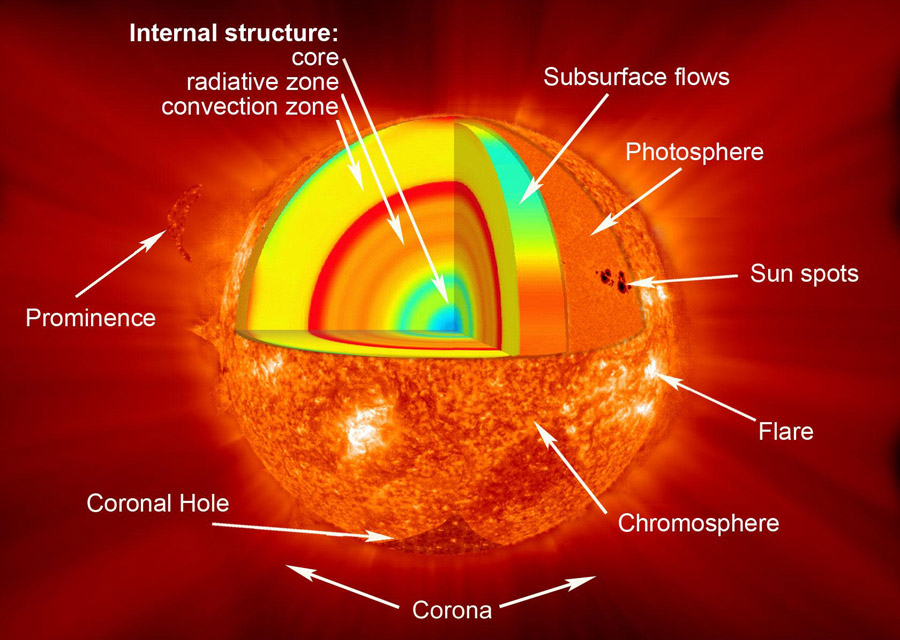
\includegraphics[width=0.5\textwidth]{images/structure_of_sun.jpg}
    \caption[Structure of the Sun]{Structure of Sun. (Image credit: NASA)}
    \label{fig:structure_of_sun}
\end{figure}

The radiations produced in the core radiates slowly outwards through this region into the convective zone, taking more than about 170,000 years to radiate through this layer. The \textbf{convective zone} is the region where the plasma, through the process of convection currents of heated and cooled gas, moves towards the surface.

\subsection{Solar Corona}

Outermost layer of the Sun's atmosphere is known as Solar Corona. It lies above the chromosphere and extends millions of kilometers into outer space. Corona can be easily viewed during solar eclipse (\cref{fig:corona_eclipse}), but can also be observed using a coronagraph. Coronagraph is a device that occults the disk of the Sun (similar to how moon occults the Sun during solar eclipse) thereby enabling easy coronal observations and analysis.

\begin{figure}[h!]
    \centering
    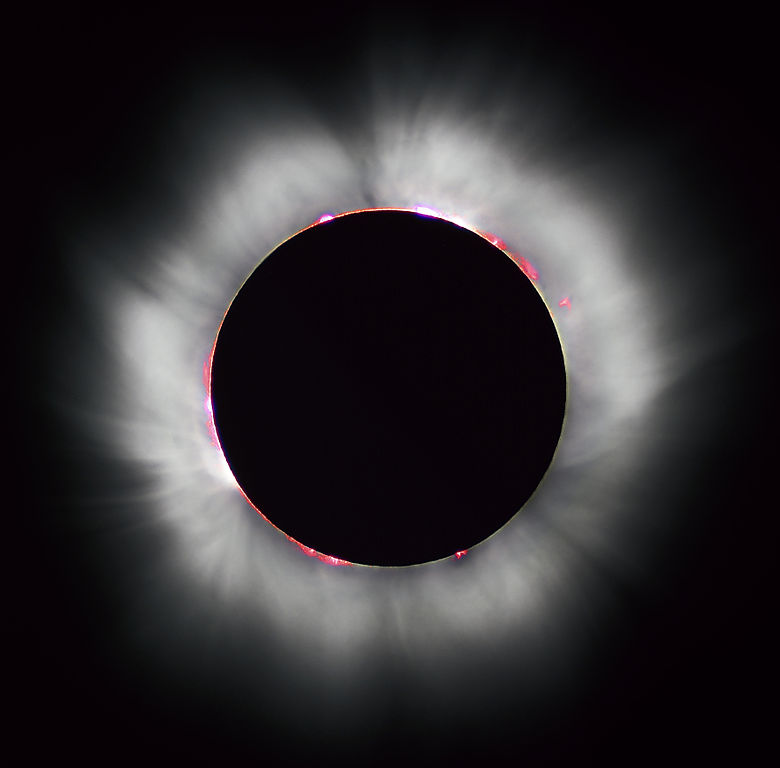
\includegraphics[width=0.5\textwidth]{images/corona.jpg}
    \caption[Image of Solar corona during a total solar eclipse]{Image of Solar corona during a total solar eclipse. (Image credit: NASA)}
    \label{fig:corona_eclipse}
\end{figure}

The temperature of solar corona is of the order of million of degree kelvin. The emitted plasma can been seen in the EUV region and it is possible to observe the corona using EUV filters without a coronagraph. The unusual spectral features of the solar corona have been explained by the existence of (Fe-XIV or Fe$^{13+}$). \citep{aschwanden2006physics}

\subsection{Solar Flares}

Explosive phenomenas that occur on the surface of sun are called as solar flares, caused by the reconnection of a sun's magnetic field lines. These flares are often accompanied by filaments/prominent eruptions and Coronal Mass Ejections (CMEs). Flares are classified into two types: \textit{eruptive} and \textit{confined}. Eruptive events are the flares which are associated with CMEs and confined flares are those which are not associated with CMEs. Plasma and magnetic field structures sometimes extend outwards from the surface. These structures are called filaments/prominences. Filaments and prominences are fundamentally of the same physical properties, only difference is the angle at which it is observed. If plasma floats outside the solar limb, it is called prominence, it is called a filament if it is within the solar background otherwise \cref{fig:filament_prominence}. Difference is in the type of spectrum obtained, which is Balmer lines in emission spectra in case of prominences and absorption lines in case of filaments. Loop-like structures of plasma stand out brightly against the dark background of space, these are prominences. An image of solar flare event of \nth{4} August 2011 is shown in \cref{fig:solar_flare_4_aug_2011}.

\begin{figure}
    \centering
    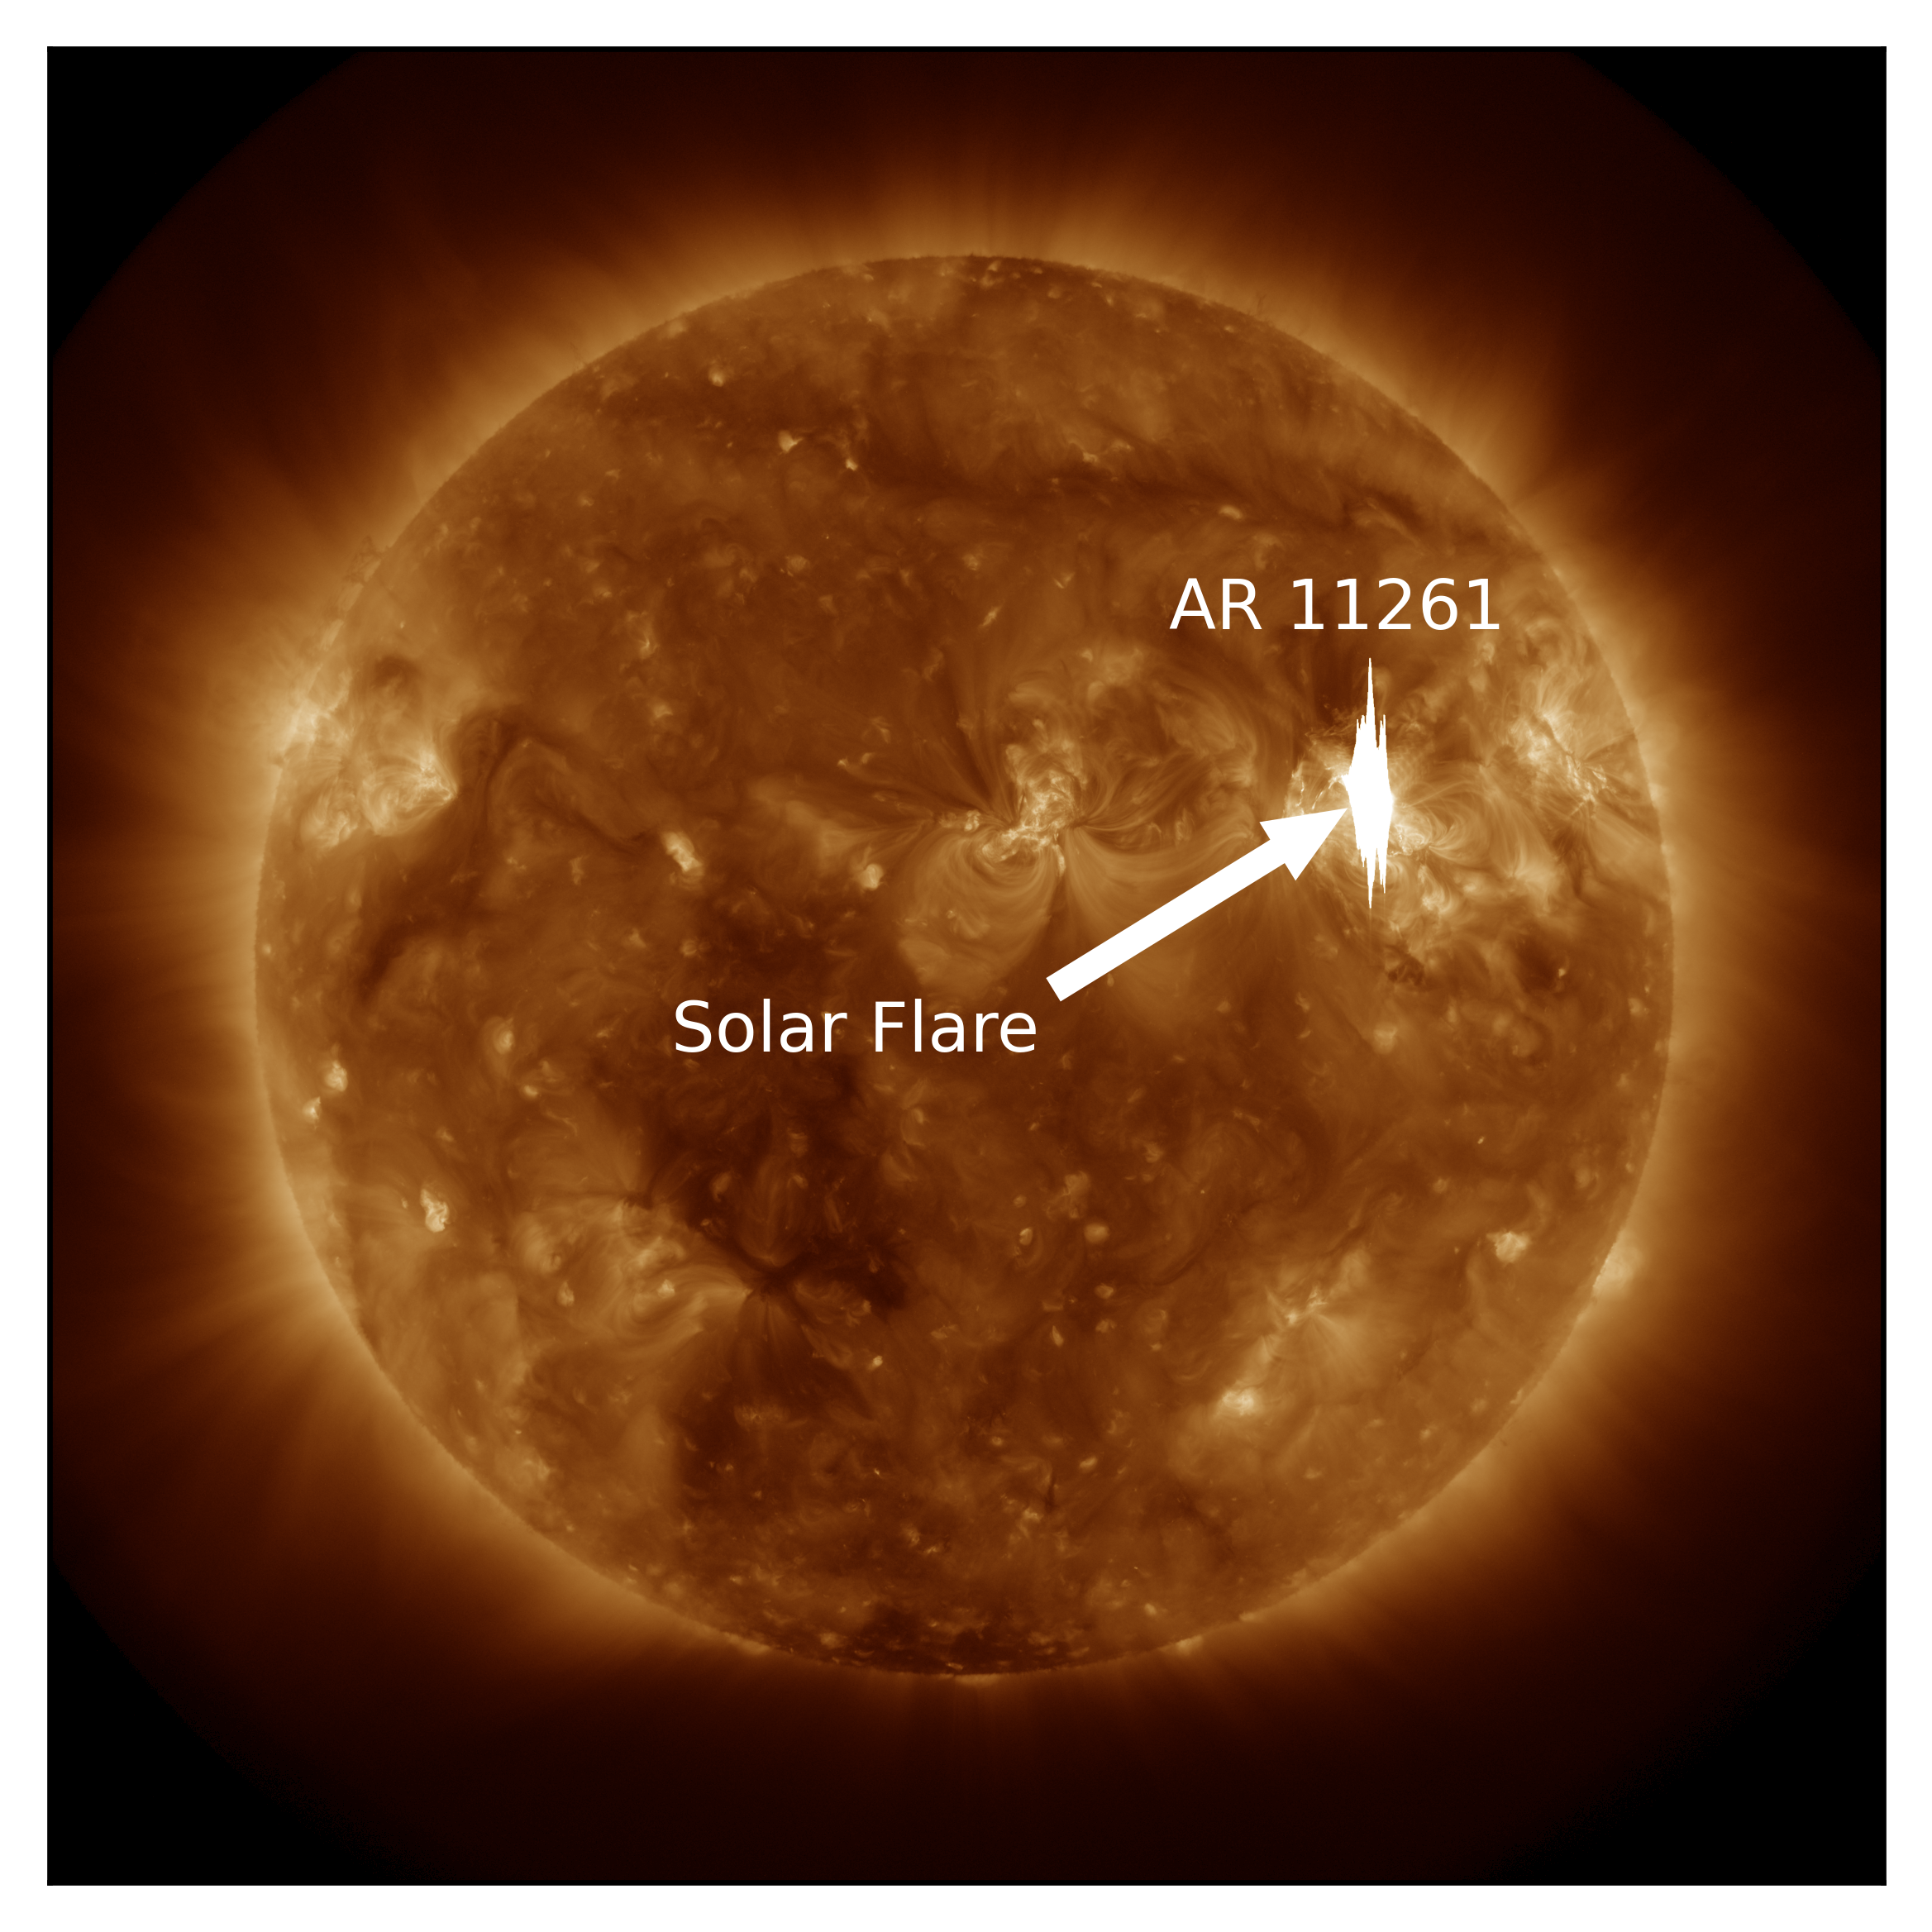
\includegraphics[width=0.5\textwidth]{images/solar_flare_4_aug_2011.png}
    \caption[Solar flare (\nth{4} August 2011)]{Solar flare event of \nth{4} August 2011 originating from the Active Region AR 11261 observed through 193 \AA \ AIA channel}
    \label{fig:solar_flare_4_aug_2011}
\end{figure}

\begin{figure}
     \begin{subfigure}[b]{0.5\textwidth}
         \centering
         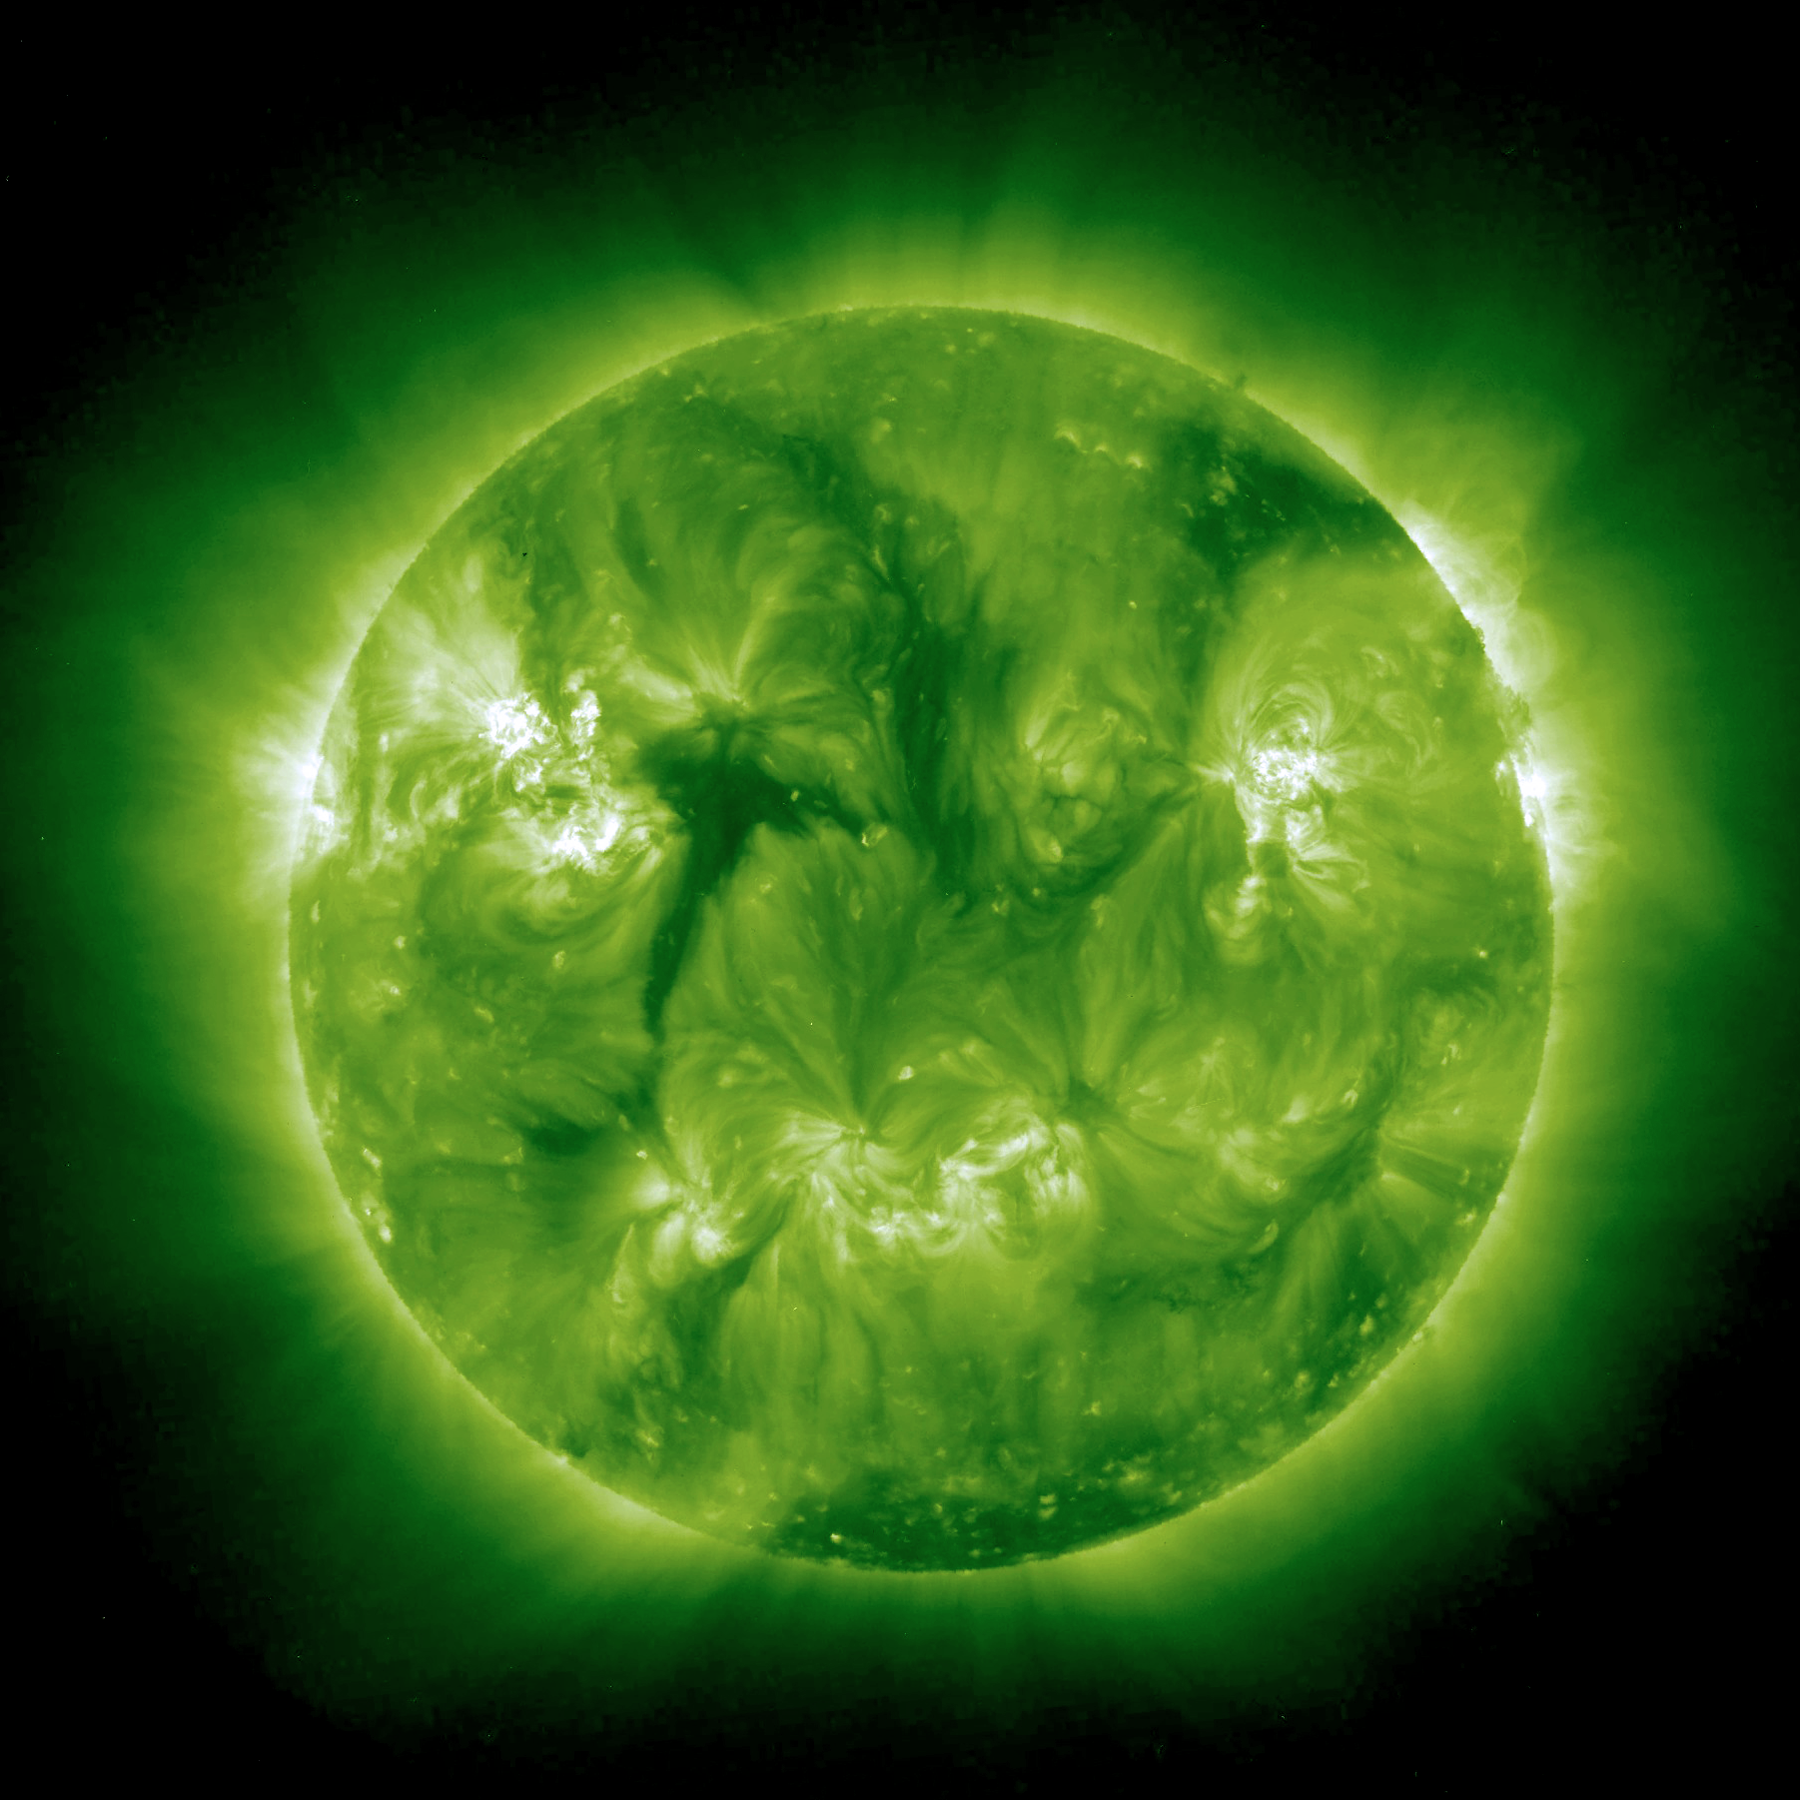
\includegraphics[width=\textwidth]{images/195_Filament.png}
         \caption{Filament}
         \label{fig:filament}
     \end{subfigure}
     \hfill
     \begin{subfigure}[b]{0.5\textwidth}
         \centering
         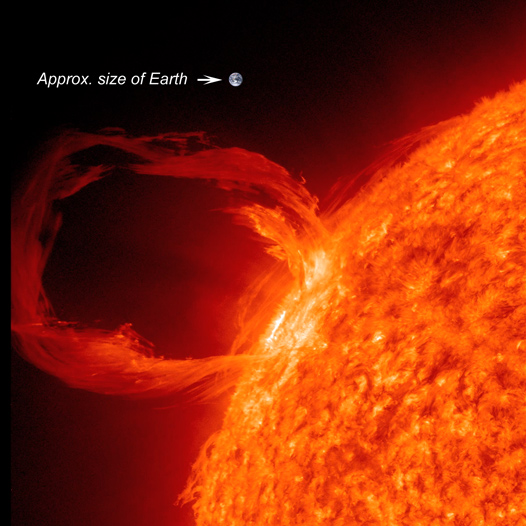
\includegraphics[width=\textwidth]{images/prominence.jpg}
         \caption{Prominence}
         \label{fig:prominence}
     \end{subfigure}
     \caption[Filament and Prominence]{\Cref{fig:filament} shows a U-shaped very long filament which was stable for a period of two days (\nth{6} - \nth{7} February 2012) . \Cref{fig:prominence} is a prominence eruption seen in Extreme UV light on \nth{30} March 2010 (credit: NASA).}
     \label{fig:filament_prominence}
\end{figure}

\subsection{Coronal Mass Ejections (CMEs)}

CMEs are large plasma structures ejected from the solar surface to the heliosphere. They were first discovered in 1971 \citep{Gopalswamy2016-nm}. They majorly affect the space weather, causes interplanetary disturbances and shock waves. CMEs propagting towards the earth can disrupt the communication technologies like satellites. Filament eruptions and solar flares are often associated with CMEs. These energetic plasma have energy of the order of $10^{29} - 10^{32}$ erg and fast speeds even up to 3600 $kms^{-1}$

\subsection{Stellar CMEs}

Similar to solar flares, stellar flares maybe associated with CMEs, but it is not easy to detect or study them as there is no spatial resolution unlike Sun. CMEs accompanied by stellar flares are substantially larger in comparison to the ones observed on the Sun, and have been known to affect the exoplanets around the host stars \citep{Veronig2021-rf}. Hence studying the CMEs is very crucial for future exoplanetary expeditions also. Indirect stellar CME detections have been explored with methods such as coronal dimming, blueshifted emission of chromospheric lines, X-ray, EUV and FUV dimming, Type-II and type-IV radio bursts etc \citep{Korhonen2016-jo}. Conceptually, stellar CMEs energetics might be thought of as an extrapolation of case of solar CME. But, \citep{Argiroffi2019} found that the ratio of stellar CMEs to the flaring energy is not found to be extrapolated version of solar case as seen in \cref{fig:stellar_cme_energy_mass_relation}.

\begin{figure}[ht]
    \centering
    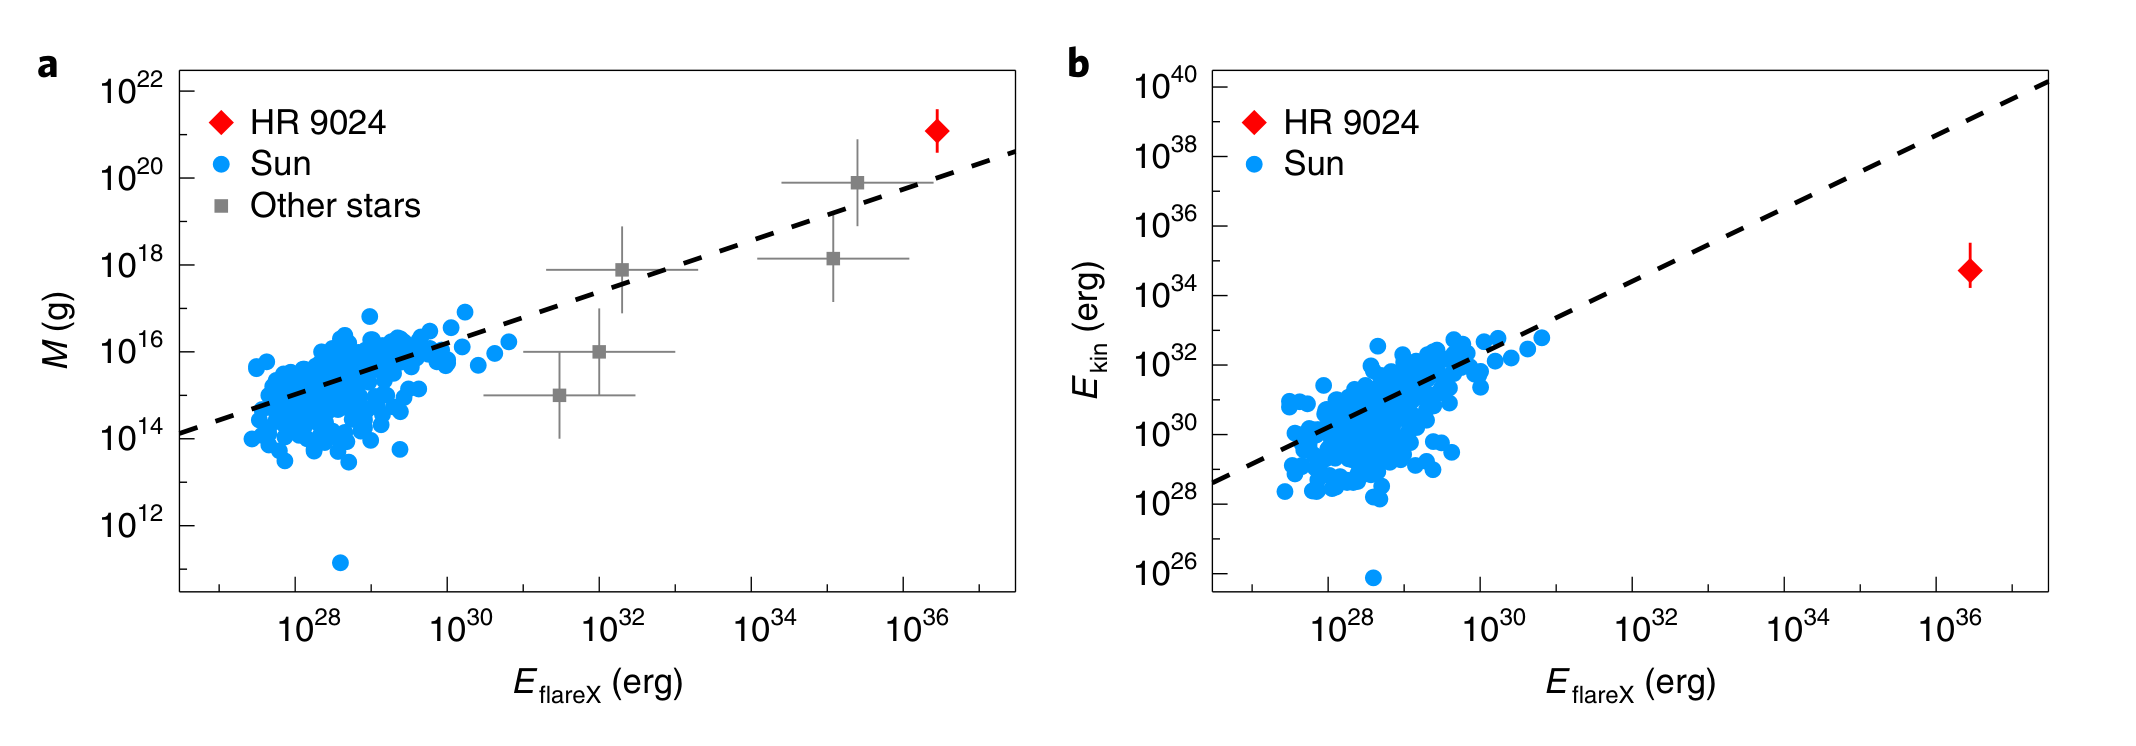
\includegraphics[width=\textwidth]{images/stellar_cme_energy_mass_relation.png}
    \caption[Extrapolation of Solar flare-CME relation]{Extrapolation of the solar flare-CME relation. Mass and kinetic energy of solar CMEs shown as a function of X-ray fluence of the associated flares. \capcite{Argiroffi2019}}
    \label{fig:stellar_cme_energy_mass_relation}
\end{figure}


\subsection{Coronal Dimming}

Coronal dimming is considered one of the promising signatures to detect the occurence of stellar CMEs \citep{Namekata2022-dm}. Regions with temporary dimming of plasma on the solar surface is seen after an eruptive event like CMEs in the EUV and soft X-ray wavelengths. This dimming observed is due to the mass loss in the corona after an eruptive event like CME \citep{Mason2014}. Dimming is most prominently observed in the 1-2 million K range of Sun's plasma of the quiet corona. Time series plot of irradiance value of Sun shows a prominent decrease after the event compared to the value before the event. This effect is known as Coronal Dimming. The probability of Coronal Dimming being associated with CMEs have been observed to be very high $P(Dim \mid CME) = 0.842$ in comparison to false alerts $P(Dim \mid !CME) = 0.167$. Probability of CMEs being associated with dimming ($P(CME \mid Dim) = 0.970$) is also very high \citep{Veronig2021-rf}. Many studies have been done to get information about the underlying CME from the coronal dimming. The depth and slope of the dimming region in the light curve during CME events have been studied and empirical formulations have been done to get information about their mass and velocity \citep{Mason2016}. \Cref{fig:dimming_5_channels} shows the coronal dimming associated with CME due to the solar flare event of \nth{4} August 2011.

\begin{figure}[h!]

    \begin{subfigure}[b]{0.3\textwidth}
        \centering
        \includegraphics[width=\textwidth]{images/dimming_211.png}
        \caption{$211 \ \AA$}
        \label{fig:dimming_211}
    \end{subfigure}
    \hfill
    \begin{subfigure}[b]{0.3\textwidth}
        \centering
        \includegraphics[width=\textwidth]{images/dimming_94.png}
        \caption{$94 \ \AA$}
        \label{fig:dimming_94}
    \end{subfigure}
    \hfill
    \begin{subfigure}[b]{0.3\textwidth}
        \centering
        \includegraphics[width=\textwidth]{images/dimming_131.png}
        \caption{$131 \ \AA$}
        \label{fig:dimming_131}
    \end{subfigure}

    \begin{center}
        \begin{subfigure}[b]{0.3\textwidth}
            \centering
            \includegraphics[width=\textwidth]{images/dimming_171.png}
            \caption{$171 \ \AA$}
            \label{fig:dimming_171}
        \end{subfigure}
        \hspace{0.5cm}
        \begin{subfigure}[b]{0.3\textwidth}
            \centering
            \includegraphics[width=\textwidth]{images/dimming_193.png}
            \caption{$193 \ \AA$}
            \label{fig:dimming_193}
        \end{subfigure}
    \end{center}
    \caption[AIA images of Coronal Dimming regions on the Sun]{AIA images of the Sun depicting coronal dimming in five of the channels in the order: 211 \AA, 94 \AA, 131 \AA, 171 \AA, 193 \AA. The two yellow dashed boxes depict the dimming region created because of the ejection of CME associated with the flare event of \nth{4} August 2011 (dimming starts around 04:21 UT).}
    \label{fig:dimming_5_channels}
\end{figure}

\subsection{Instrument}

\begin{figure}[h!]
    \centering
    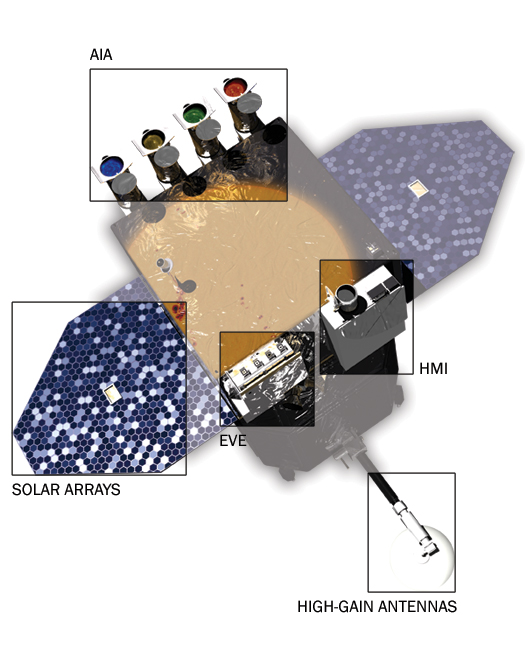
\includegraphics[width=0.5\textwidth]{images/spacecraft_detailed.jpg}
    \caption[SDO Spacecraft]{Solar Dynamics Observatory Spacecraft.
      Image obtained from {\url{https://sdo.gsfc.nasa.gov/mission/spacecraft.php}}}
    \label{fig:sdo_spacecraft}
\end{figure}

We are using Atmosphere Imaging Assembly (AIA) instrument of Solar Dynamics Observatory (SDO; \citep{Pesnell2011})(\cref{fig:sdo_spacecraft}) for the Sun's spectral irradiance data. SDO is a space observatory launched by NASA on 2010 as a part of `Living With a Star' (LWS) program. The spacecraft contains three instruments on board: Extreme Ultraviolet Variability Experiment (EVE), Helioseismic and Magnetic Imager (HMI), Atmospheric Imaging Assembly (AIA). We'll be focusing on the AIA instrument, since that is what we are using. AIA was built in partnership with Lockheed Martin Solar and Astrophysics Laboratory (LMSAL). AIA contains 4 cassegrain telescopes which are optimized to observe narrow bands in the EUV region. Each of the four f/20 telescope has a 20-cm primary mirror and an active secondary mirror. The telescope is designed to prevent charged particles from reaching the Charge Coupled Device (CCD). Field of View (FOV) of each of the telescope is 41 arcmin in circular diameter. The mirrors have special multilayer coatings that are optimized to observe the selected EUV wavelengths of interest. Three of the telescopes have two different EUV bandpasses. The CCDs are back-thinned and back-illuminated with 4096 $\times$ 4096 pixels capturing capabilities. Each of the 12 $\mu$m pixel corresponds to 0.6 arcsec. The telescopes have a selector mechanism to choose the wavelength. AIA captures full-frame EUV image and one UV or visible-light image every 12 seconds. \citep{Lemen2011}\\

\begin{table}[h!]
    \centering
      \setlength{\tabcolsep}{10pt}
      \renewcommand{\arraystretch}{1.5}
    \begin{tabular}{| l | l | l | l |}
      \hline
       \textbf{Band} & \textbf{Primary role, ion(s)} & \textbf{Region of Sun's atmosphere} & \textbf{logT{[}K{]}} \\
      \hline
      4500 Å & Continuum            & Photosphere                                            & 3.7                                   \\
      \hline
      1700 Å & Continumm            & Temperature minimum, photosphere                       & 3.7                                   \\
      \hline
      304 Å  & He II                & Chromosphere, transition region                        & 4.7                                   \\
      \hline
      1600 Å & C IV, continumm      & Transition region, upper photosphere                   & 5.0                                   \\
      \hline
      171 Å  & Fe IX                & Quiet corona, upper transition region                  & 5.8                                   \\
      \hline
      193 Å  & Fe XII, XXIV         & Corona and hot flare plasma                            & 6.1, 7.3                              \\
      \hline
      211 Å  & Fe XIV               & Active region corona                                   & 6.3                                   \\
      \hline
      335 Å  & Fe XVI               & Active region corona                                   & 6.4                                   \\
      \hline
      94 Å   & Fe XVIII             & Flaring regions                                        & 6.8                                   \\
      \hline
      131 Å  & Fe XX, XXIII         & Flaring regions                                        & 7.0, 7.2                              \\
      \hline
    \end{tabular}
    \caption{AIA wavelength channels. Table obtained from \url{https://aia.lmsal.com/public/instrument.htm}}
    \label{tab:aia_wav_channels}
\end{table}

\begin{figure}[h!]
    \begin{subfigure}[b]{0.5\textwidth}
        \centering
        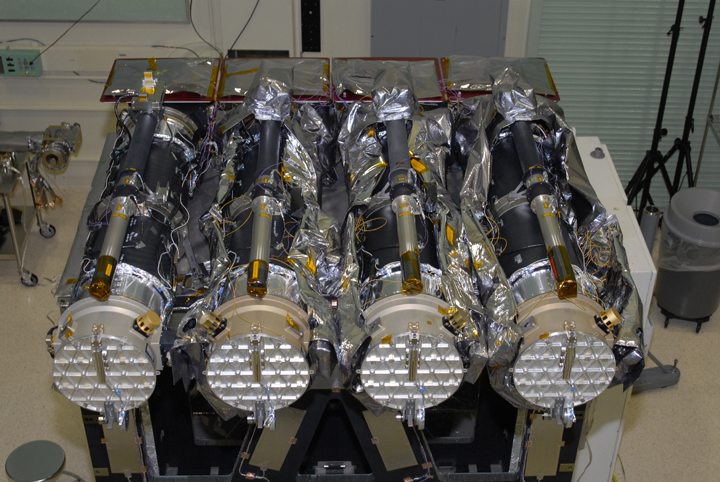
\includegraphics[width=\textwidth]{images/SDO AIA Telescopes.jpg}
        \caption{ }
        \label{fig:aia_telescopes}
    \end{subfigure}
    \hfill
    \begin{subfigure}[b]{0.5\textwidth}
        \centering
        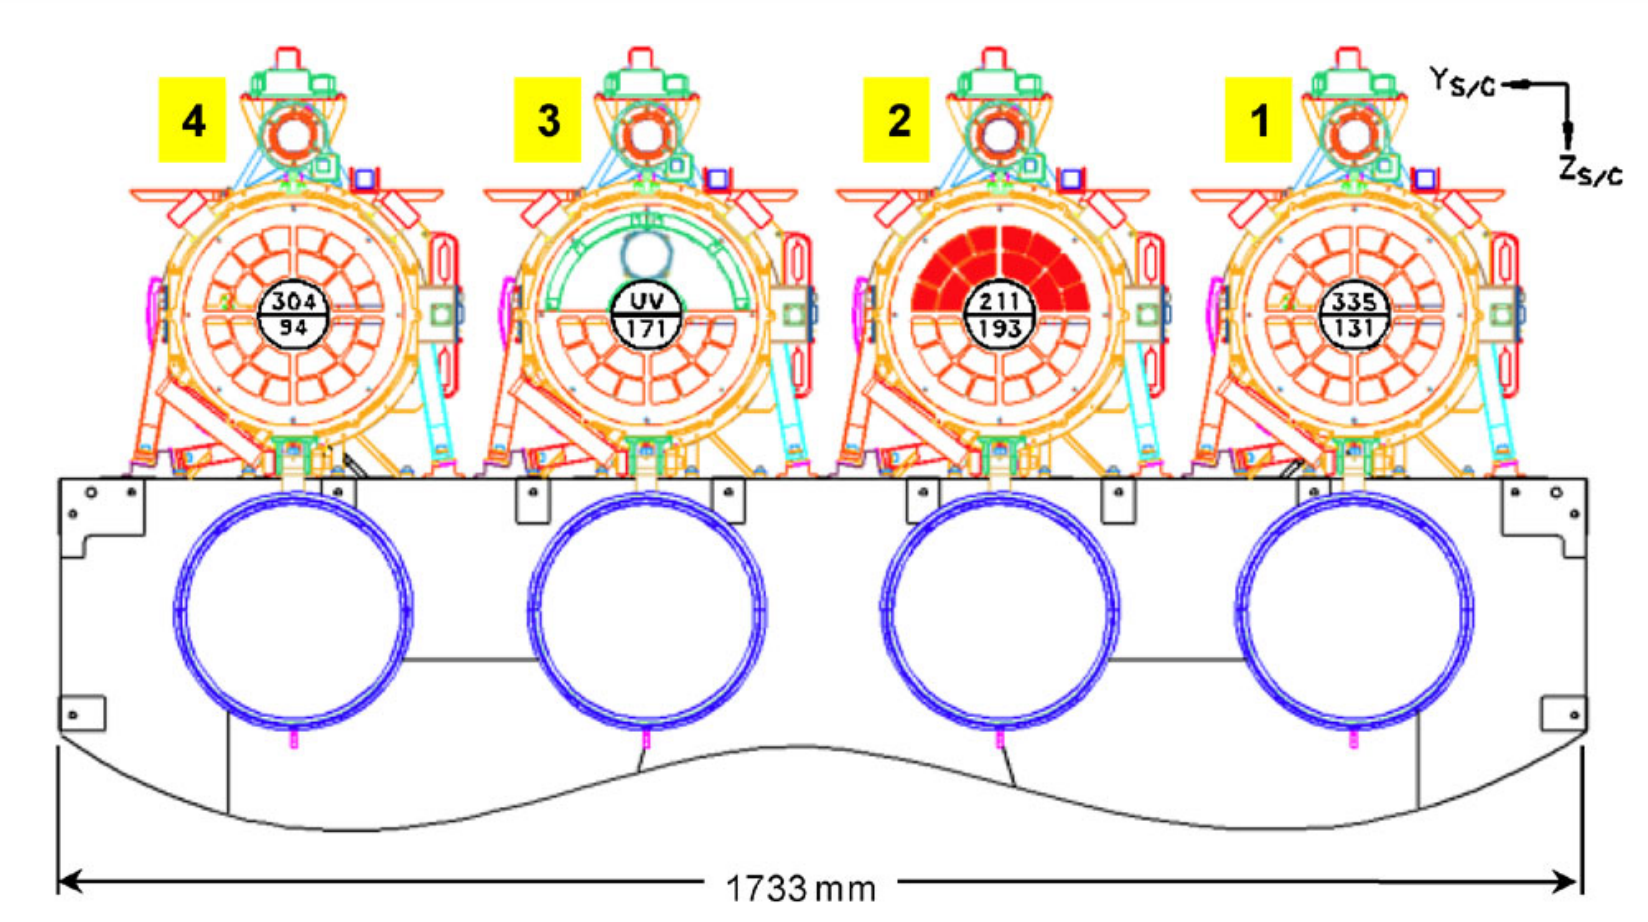
\includegraphics[width=\textwidth]{images/AIA_telescope_layout.png}
        \caption{ }
        {\label{fig:aia_telescope_layout}}
    \end{subfigure}
    \label{fig:aia_telescope_and_layout}
    \caption[AIA telescope and it's Layout]{\Cref{fig:aia_telescopes} shows the AIA telescopes. \Cref{fig:aia_telescope_layout} shows the AIA telescope layout. Telescope 2 has an aperture blade to select between it's two wavelength channels. Rest of the telescopes rely on the filters in filter wheels to select the channel (Image credit: \capcite{Lemen2011})}
\end{figure}

The different channels of AIA respond differently to the radiation of different temperature. The channels of AIA along with it's primary role, region of Sun's atmosphere it probes and temperature has been given in \cref{tab:aia_wav_channels}. The response of the instrument to different wavelengths and temperature is given by it's response curves, which are of two types: \textit{wavelength response curve} and \textit{temperature response curves}. Temperature response curves gives the information about the response of each channel with respect to the temperature of the radiation being received. Temperature response curves play a crucial role in DEM analysis.

\noindent \Cref{fig:aia_tresp} shows the response curves, which has been obtained using \texttt{aia\_get\_response.pro} procedure of SSW IDL.

\begin{figure}[h!]
    \centering
    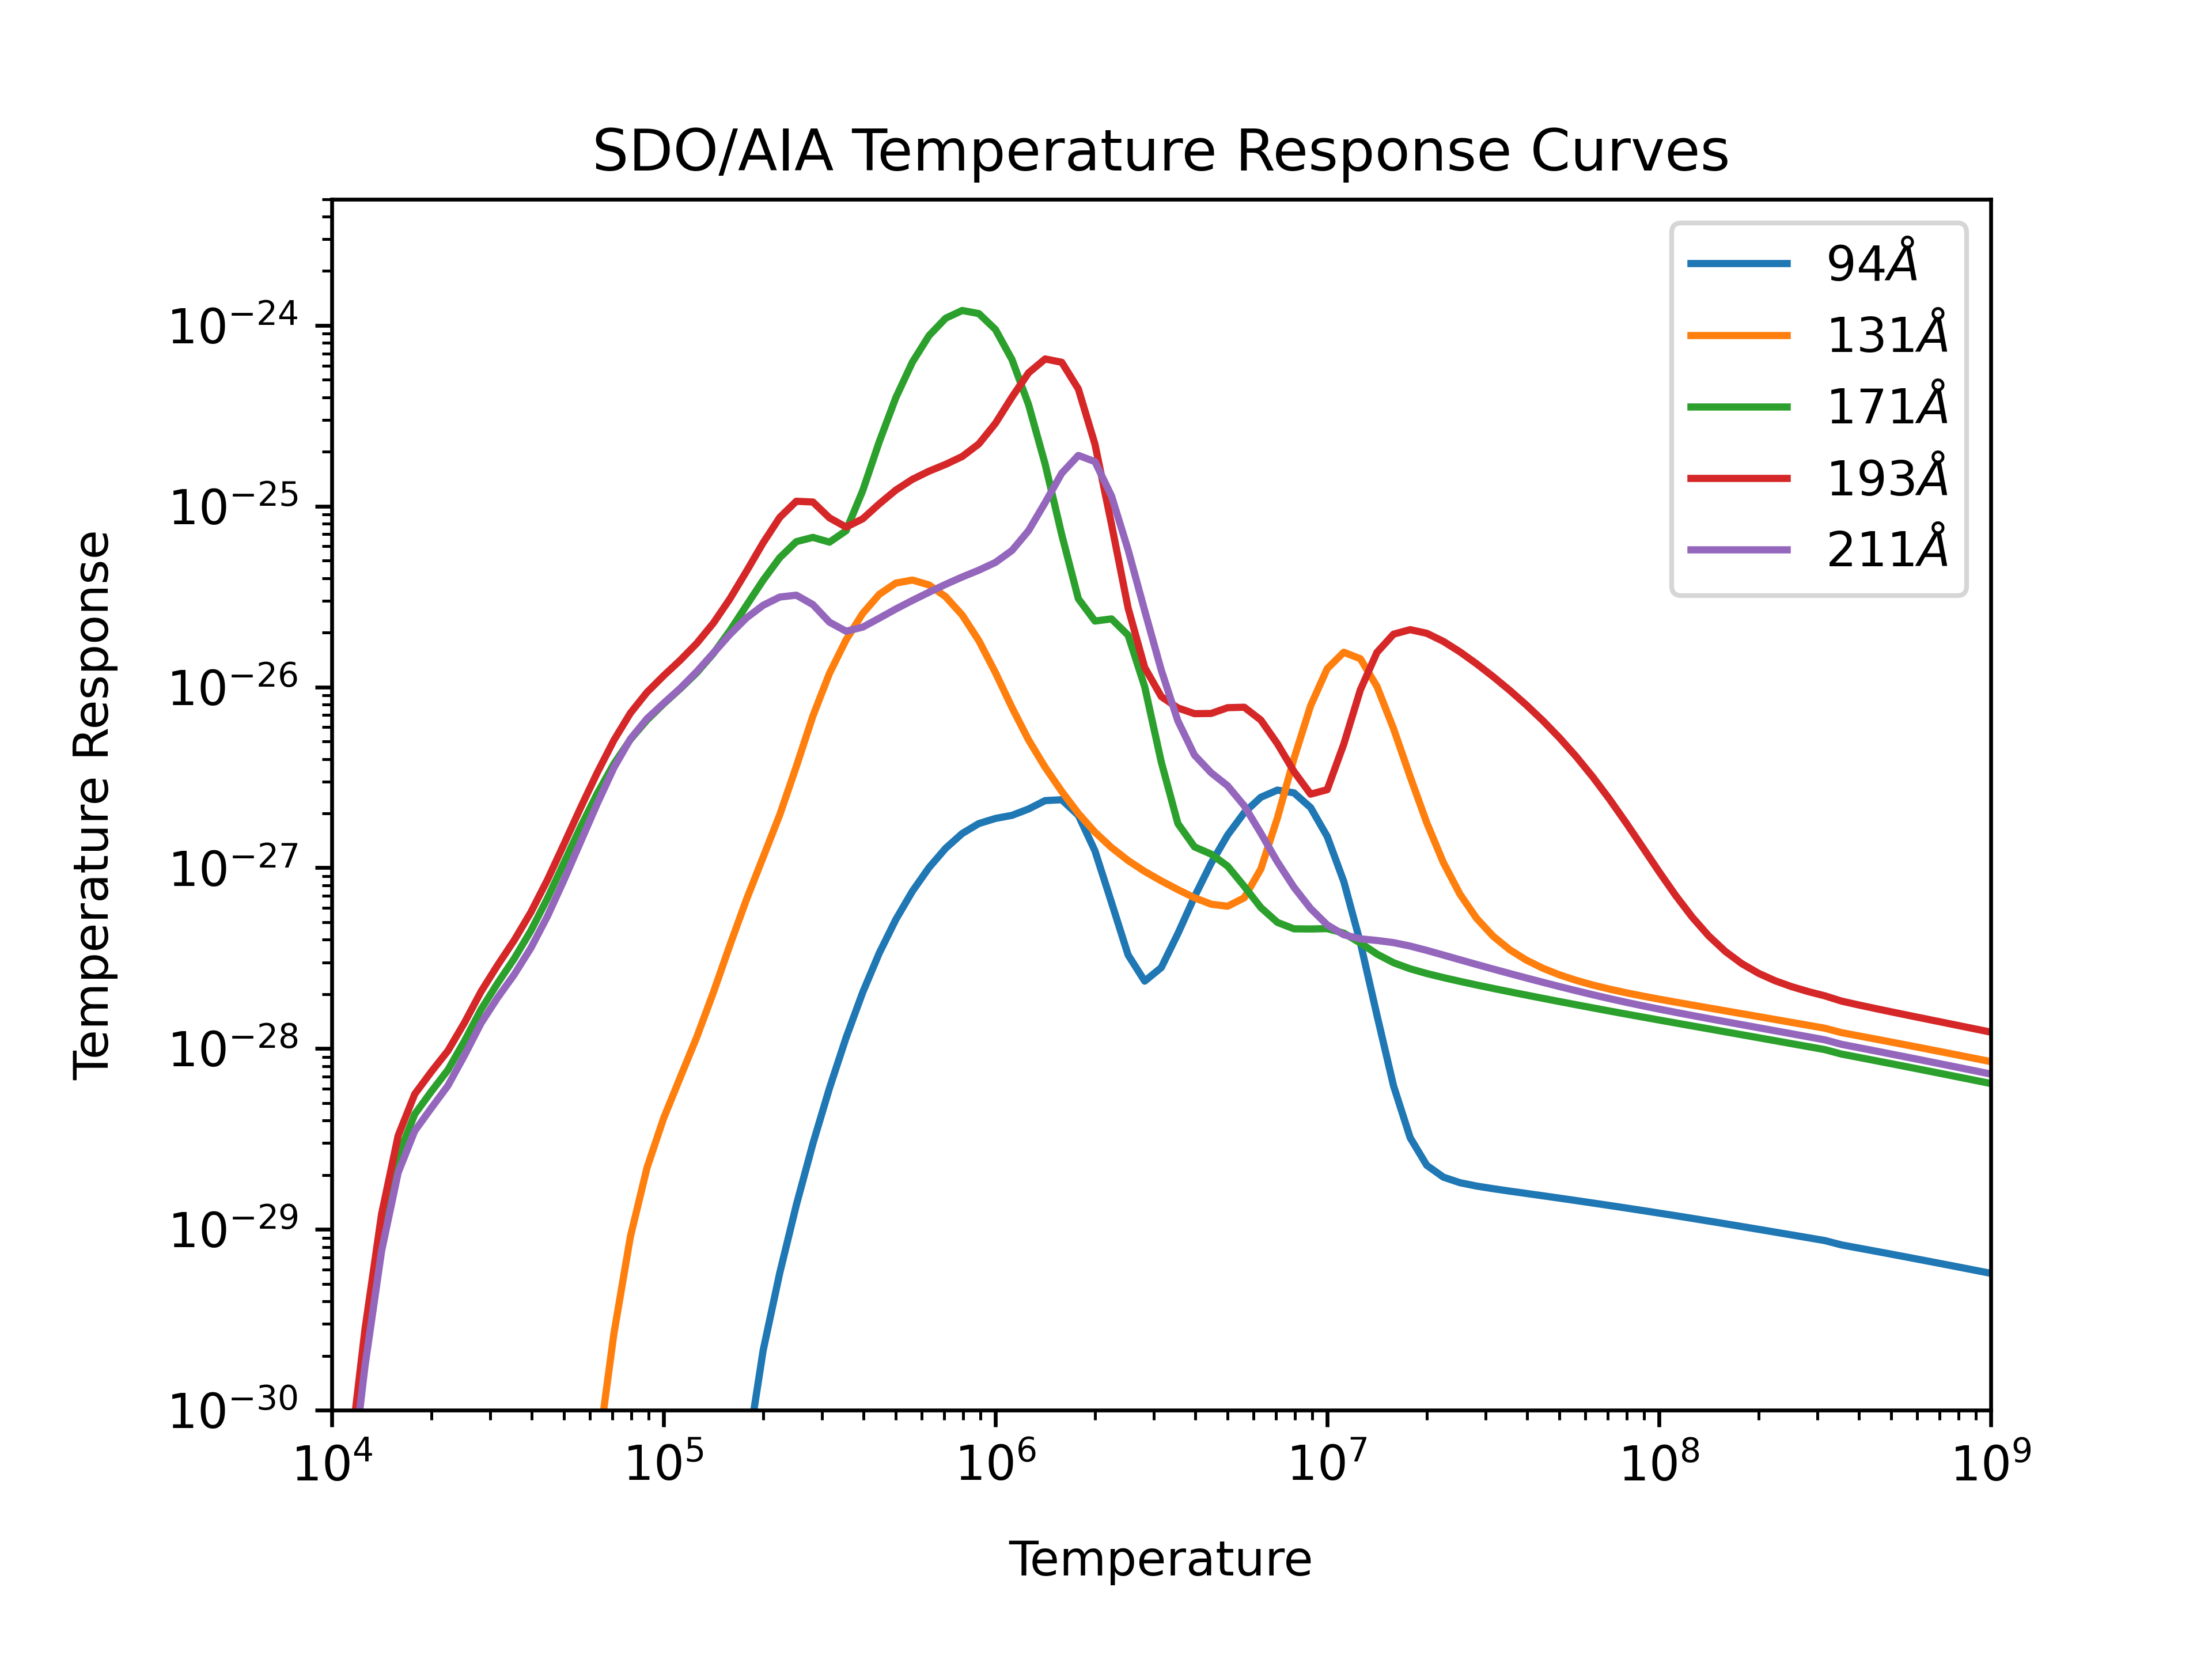
\includegraphics[width=0.75\textwidth]{images/aia_tresp.png}
    \caption[AIA Temperature Response Curves]{SDO/AIA Temperature Response Curves obtained using \texttt{aia\_get\_response.pro}. Curves corresponding to the five wavelength channels required for the DEM analysis has been plotted. Temperature has the unit of Kelvin and temperature response function has the unit of [DN $cm^5 s^{-1} pixel^{-1}$]}
    \label{fig:aia_tresp}
\end{figure}

%%% Local Variables:
%%% mode: LaTeX
%%% TeX-master: "main"
%%% End:


\section{Literature Review}

The motivation for indirect detection of CMEs from Sun has led researchers to find out association of CMEs with eruptive events on the Sun like Solar flare, filament and prominence eruptions, coronal dimming associations with CME and vice-versa etc. About 73 \% association of CME events with eruptive filaments  has been observed \citep{Sinha2019}. It has been demonstrated that EM distributions from SDO/AIA data alone can overestimate the amount of high temperature (logT \textgreater\ 6.4) plasma in the solar corona by a factor of 3-15 \citep{Athiray2024}. Coronal dimming phenomenas have been extensively studied and many empirical formulations have also been derived to get information about the underlying CMEs like mass and velocity of the CMEs ejected by knowing the depth and slope of the dimming curve \citep{Mason2016}. The association of dimming with a CMEs and assocation of CME with dimming has been observed to be very high ($P(Dim \mid CME) = 0.842$, $P(Dim \mid !CME) = 0.167$, $P(CME \mid Dim) = 0.970$) \citep{Veronig2021-rf}. Sun-as-a-star analysis methods have been used widely for comparing and studying stellar and solar CMEs. Multi-temperature structure analysis of stellar active phenomena in spatially integrated spectra is allowed by the combination of H$\alpha$ and EUV lines, instead of single spectra analysis \citep{Otsu2024}. Redshifted components of stellar filament eruptions in Sun-as-a-star analysis in H$\alpha$ spectra may develop into CMEs \citep{Otsu2022}. Further studies into stellar CMEs connecting the CME mass and velocity to the stellar flare energy, leading to the conclusion that stellar CMEs are restricted in terms of their velocity due to the strong stellar magnetic fields and stellar wind drag \citep{Moschou2019-zq}. One expects that the case of stellar CME in terms of it's energetics and association to stellar flares will be a scaled version of the solar CMEs, but discrepancy has been found in terms of the ratio between the Kinetic energy of stellar CME to the stellar flaring energy not being anywhere close to being a scaled version of the solar case \citep{Namekata2022-dm}.

%%% Local Variables:
%%% mode: LaTeX
%%% TeX-master: "main"
%%% End:


\section{Methodology}

In this study, we use the SDO/AIA data of the Sun for three particular CME events (\cref{sec:selection_of_events}). These events are associated with special features like coronal dimming, filament eruptions and GLE event. The DEM for each image of the three events is obtained using the RML method. Next, we convert the full disk image of Sun to a point source (hereafter referred to as \textbf{Pointification}) and then inspecting if the signatures of the CMEs exist after the conversion and is similar to what is was before the conversion. Pointifying the Sun roughly translates to converting Sun to a star, or placing Sun to a place that's distant from Earth/observer in comparison to the distance between us and the Sun (defined as astronomical unit (1 AU $\approx 1.496\times10^{8}$ km)) such that it appears as a point source. We then analyse and compare the irradiance from the point source Sun and the full disk Sun using DEM to see if they show similar signatures of CMEs. Typically, Sun-as-a-star analysis involves selecting a region of interest on the surface of the Sun, making the assumption that this is the only region that affects the event under study, and that there is no activity anywhere on the rest of the Sun's surface, and then integrating the parameter of interest over the entire Solar disk. This is again a rough approximation to an actual star. Coronal dimming associated event is investigated to find the temperature range that shows the maximum amount of dimming.\\

In the following section, we discuss about the analysis tools used (\cref{sec:data_analysis_tools_used}), selection of events (\cref{sec:selection_of_events}), data used for the study (\cref{sec:data_used}), data pre-preprocessing (\cref{sec:data_pre_processing}) and data analysis procedure (\cref{sec:data_analysis_procedure}).

  \subsection{Data Analysis tools used}
  \label{sec:data_analysis_tools_used}

We have made use of Python programming language for our analysis. We have made extensive use of the following libraries: Numpy, Scipy, Aiapy, Sunpy, Pandas, Matplotlib, Astropy, Natsort, Multiprocessing, Datetime, Moviepy. In addition, we have used the RML method code for DEM analysis, as mentioned in \citep{Massa2023}. We have made use of SSW IDL for obtaining the temperature response curves for AIA. For visual inspection of the CME events, we have used JHelioViewer software. For quick inspection of the FITS file data, we have used FITSExplorer \footnote{link to the github repo: \url{https://github.com/dheerajshenoy/FITSExplorer}}, a software created as a side project by Dheeraj Vittal Shenoy.

\subsection{Event Selection}
\label{sec:selection_of_events}

We have chosen three CME events that have erupted on 2011 August 04, 2012 August 31 and 2021 October 28. The Solar and Heliospheric Observatory's  (SOHO) Large Angle and Spectrometric Coronagraph Experiment (LASCO) C2 (SOHO/LASCO) images of the CMEs obtained from the SOHO/LASCO CME catalog (\url{https://cdaw.gsfc.nasa.gov/CME_list/}) are given in \cref{fig:cme_events_soho_pics} (running difference image) and \cref{fig:cme_events_soho_pics_aia193} (C2 image with AIA 193 $\AA$ filter). Brief description of the events is given below:\\

\begin{enumerate}

        \item\textbf{2011 August 04}: This event has been refered from \citep{Mason2016} in which it is the \nth{20} Event. The event started at around 04:12 UT. This event occured from the source location N19W36 associated with the active region AR 11261.\\

        \item\textbf{2012 August 31}: This CME event was associated with a long filament eruption and it erupted around 19:49 UT. The CME associated with the filament travelled at over 900 miles per second.\\

    \begin{figure}[h!]
        \centering
        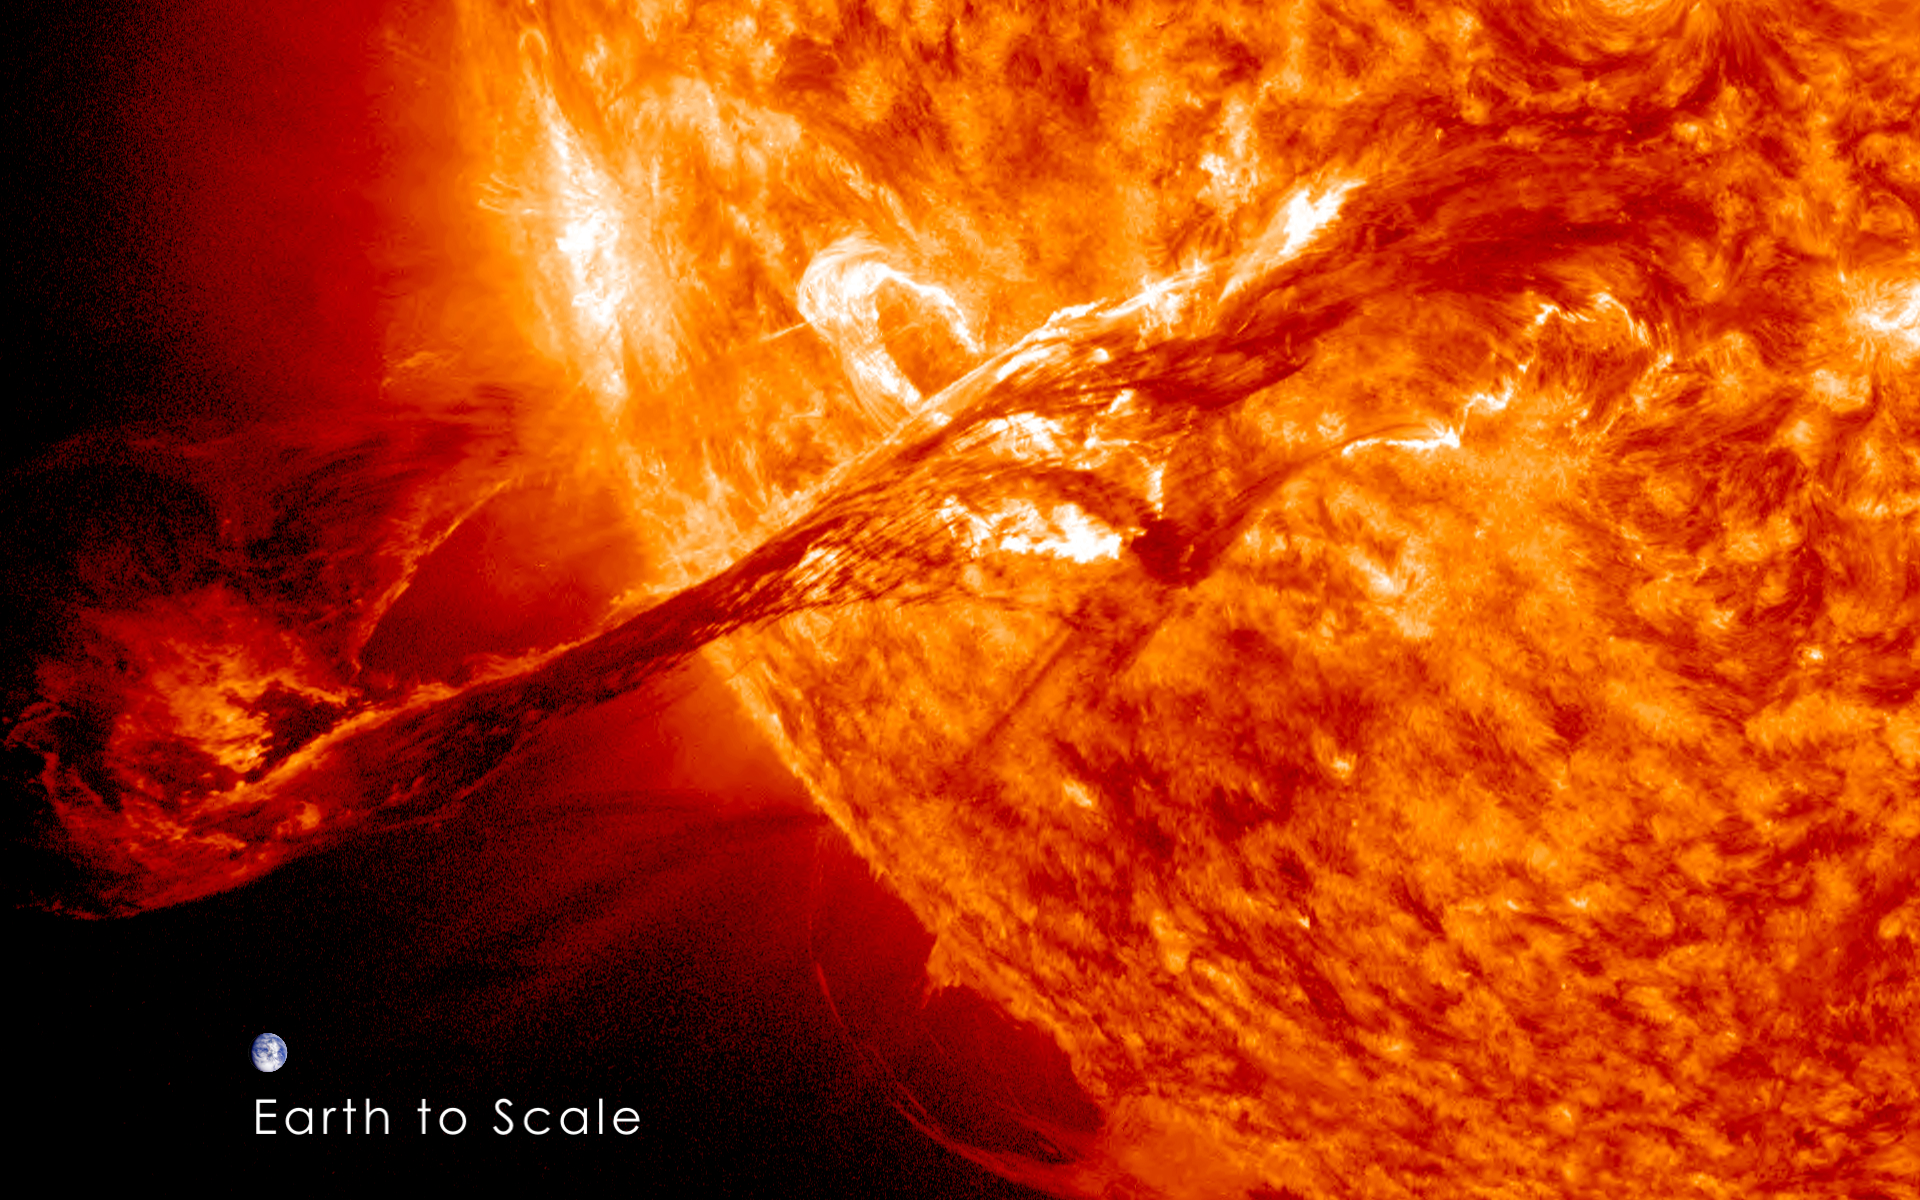
\includegraphics[width=0.5\textwidth]{images/aug_31_2012_event_sun_earth_image.jpg}
        \caption[Image of the Earth to scale of the 2012 August]{Image of the Earth to scale with the filament eruption of \nth{31} August 2012. Image credit: \url{https://svs.gsfc.nasa.gov/11095}}
        \label{fig:sun_earth_aug_31_2012}
    \end{figure}

        \item\textbf{2021 October 28}: This is an example for rarely occuring `ground level enhancement' event. During such an event, particles from the Sun are energetic enough to pass through the magnetic sheath that surrounds Earth and protects us from low energy solar outbursts. This was only the 73rd ground level enhancement since records began in the 1940s, and none have been recorded since \citep{Klein2022}. The event occured around 15:17 UT. The flare associated with the CME was an X1.1 class flare originated from the active region AR 2887.\\

\end{enumerate}

\begin{figure}[h!]
    \begin{subfigure}[b]{0.3\textwidth}
        \centering
        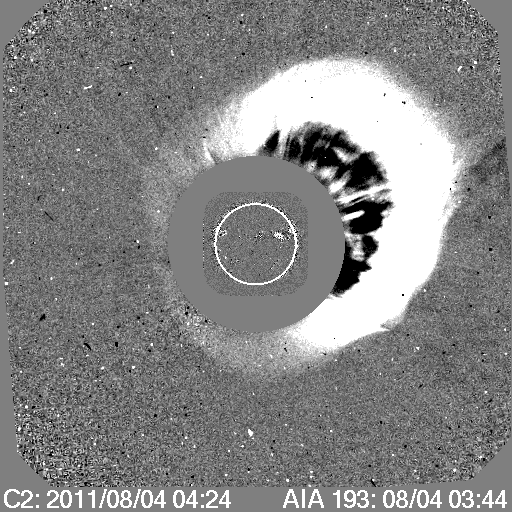
\includegraphics[width=\textwidth]{images/soho_cme_aug_04_2011.png}
        \caption[August \nth{4} 2011 CME]{August \nth{4} 2011}
        \label{fig:soho_cme_aug_04_2011}
    \end{subfigure}
    \hfill
    \begin{subfigure}[b]{0.3\textwidth}
        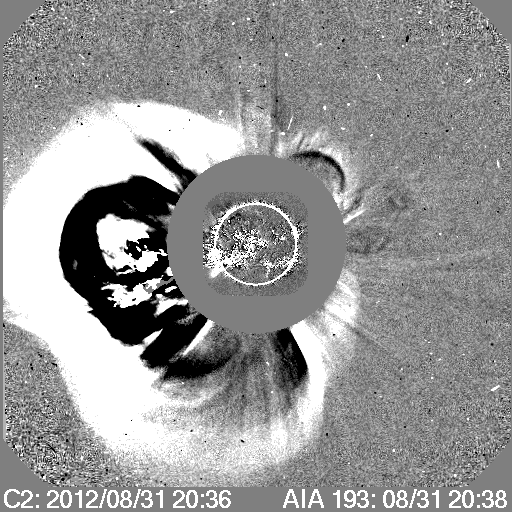
\includegraphics[width=\textwidth]{images/soho_cme_aug_31_2012.png}
        \caption[August \nth{31} 2012 CME]{August \nth{31} 2012}
        \label{fig:soho_cme_aug_31_2012}
    \end{subfigure}
    \hfill
    \begin{subfigure}[b]{0.3\textwidth}
        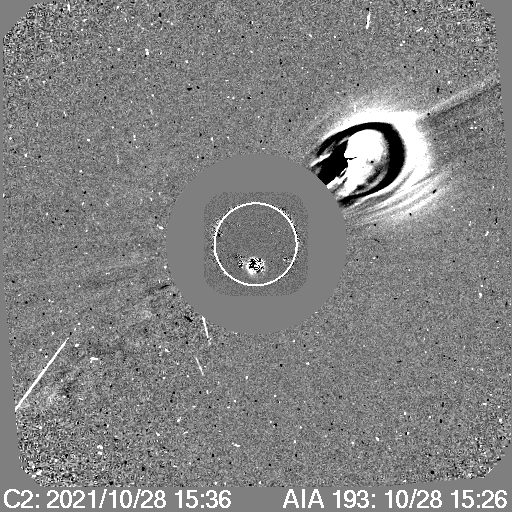
\includegraphics[width=\textwidth]{images/soho_cme_oct_28_2021.png}
        \caption[October \nth{28} 2021]{October \nth{28} 2021}
        \label{fig:soho_cme_oct_28_2021}
    \end{subfigure}
    \caption[SOHO/LASCO C2 running difference images of the selected events]{SOHO/LASCO C2 running difference images of the three selected events}
    \label{fig:cme_events_soho_pics}
\end{figure}

\begin{figure}[h!]
    \begin{subfigure}[b]{0.3\textwidth}
        \centering
        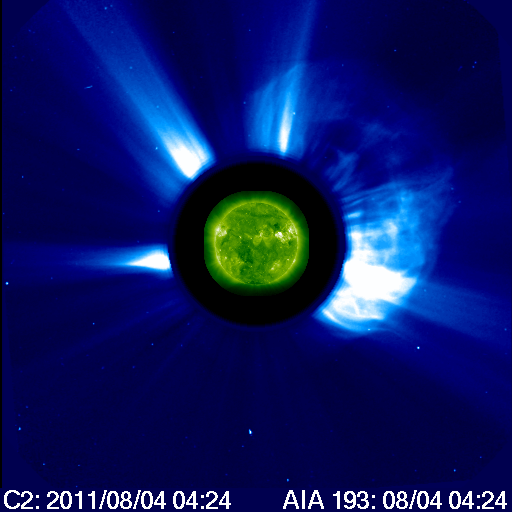
\includegraphics[width=\textwidth]{images/soho_cme_aug_04_2011_aia193.png}
        \caption[August \nth{4} 2011 CME]{August \nth{4} 2011}
        \label{fig:soho_cme_aug_04_2011}
    \end{subfigure}
    \hfill
    \begin{subfigure}[b]{0.3\textwidth}
        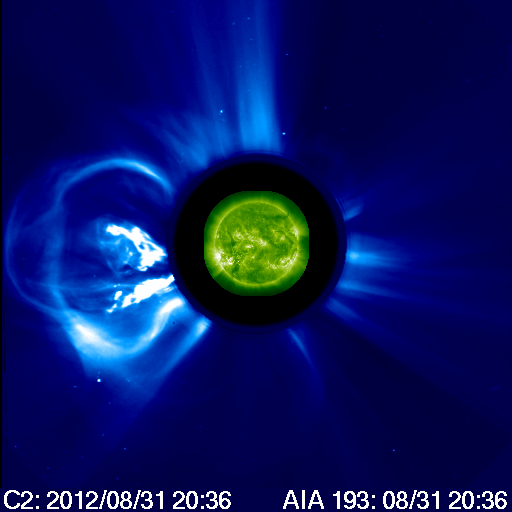
\includegraphics[width=\textwidth]{images/soho_cme_aug_31_2012_aia193.png}
        \caption[August \nth{31} 2012 CME]{August \nth{31} 2012}
        \label{fig:soho_cme_aug_31_2012}
    \end{subfigure}
    \hfill
    \begin{subfigure}[b]{0.3\textwidth}
        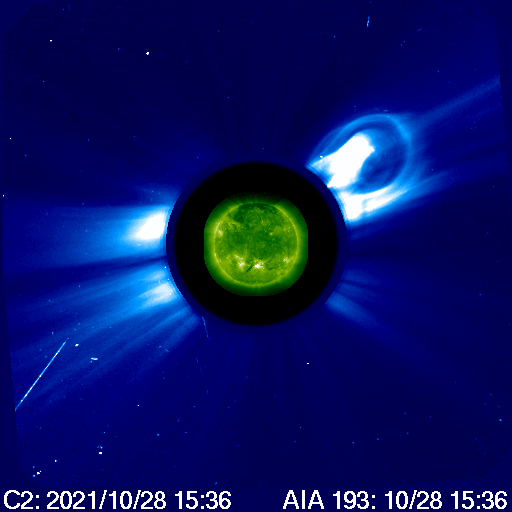
\includegraphics[width=\textwidth]{images/soho_cme_oct_28_2021_aia193.png}
        \caption[October \nth{28} 2021]{October \nth{28} 2021}
        \label{fig:soho_cme_oct_28_2021}
    \end{subfigure}
    \caption[SOHO/LASCO C2 images with AIA 193 \AA filter]{SOHO/LASCO C2 AIA 193 \AA\ filter images of the three selected events}
    \label{fig:cme_events_soho_pics_aia193}
\end{figure}

\subsection{Data}
\label{sec:data_used}

The SDO/AIA data is accessed through the JSOC portal (\url{http://jsoc.stanford.edu}) and required event data is obtained through the service. Event data consists of FITS files of Sun's image for the selected wavelength bands. For our analysis, we have used 5 channels: 94 $\AA$, 131 $\AA$, 171 $\AA$, 193 $\AA$ and 211 $\AA$. The remaining channels probe the Sun's surface temperature that is greater than what is required for our analysis. Also, the 335 $\AA$ channel has been excluded because of it's relatively weak temperature response at any temperature which affects the RML method used for the DEM analysis \citep{Massa2023}. We have used 10 hours of data for the \nth{4} August 2011 and \nth{31} August 2012 events, and about 7 hours of data for the \nth{28} October 2021 event. All three event data are at 2 minute cadence (Cadence refers to the frequency or timing of observations or measurements taken of the Sun or solar phenomena. It represents how often data is collected over a period of time).

\subsection{Image Pre-Processing}
\label{sec:data_pre_processing}

The downloaded FITS data files are 4096 $\times$ 4096 pixels in dimension. Data downloaded from the portal is level 1, which has been flat-fielded and processed to remove bad pixels and spikes (only for EUV channels), but not registered to preserve precise pixel values. As different channels of AIA have different roll angles, multi-wavelength analysis of any kind with level 1.0 data is problematic. Also, the pointing information contained in the headers of these FITS images will not be accurate, as it would have undergone changes compared to the information stored when the image was created. As mentioned in the SDO Data Analysis Guide, we have to use \texttt{aia\_prep.pro} function in Solar Software (SSW) IDL to correct or prepare the data used. Additionally, the images are downscaled from their original 4096 $\times$ 4096 pixel dimension to 512 $\times$ 512 pixels using sunpy as obtaining DEM solutions for the 4k dimension would be really time consuming and unnecessary as we are comparing full disk and point source DEM solutions.\\

\noindent
The \textbf{aiapy} library is used to carry out the necessary procedure like `\textbf{Pointing correction}' and `\textbf{Registration}' as mentioned in the documentation of aiapy, to convert level 1 data to level 1.5. Pointing correction updates the keywords in the header of the FITS file to the latest information and Registration rotates, scales and translates the image so that the Solar north is aligned with the solar north and each pixel is 0.6 arcsec cross, and the center of the Sun is at the center of the image. Now, after this calibration, the images are good for multi-wavelength analysis. Finally, the images are normalized with respect to their exposure time. This is done because the images are captured under different lighting conditions or exposure settings, which leads to incorrect analysis when performing a multi-wavelength comparison. Without this, differences in brightness due to varying exposure times could distort interpretations and analysis.

\subsection{DEM Analysis}
\label{sec:dem_analysis}

Direct analysis of light curve might seem like a good choice as the effects of CMEs are seen in light curves too. But, light curve alone doesn't have any information about the temperature of the plasma that is being expelled. Information regarding the temperature can be derived using Differential Emission Measure (DEM) solutions obtained using the images of Sun. This allows us to understand the plasma temperature variations during eruptive events.

\subsubsection{Emission Measure}

Emission measure (EM) is a quantity used in astrophysics to describe the amount of emitting material along the line of sight in a particular column length or volume, usually in the context of a hot or ionized gas, such as a stellar atmosphere. It provides a measure of the emission intensity of a given region at various temperatures. It is expressed in units of $cm^{-3}$ or $cm^{-5}$, representing the number of electrons  emitting radiation measure in given volume or area respectively.

Emission measure is related to the number density of electrons $n_e$, in a column length $dh$ of plasma, along the line of sight, given by,

\vspace{-0.75cm}
\begin{center}
    \begin{equation}
        EM = \int_h n_e^2 \hspace{0.1cm} dh
    \end{equation}
\end{center}

Emission measure is a crucial parameter in understanding the energetics and physical conditions of a plasma, such as those found in stars, galaxies and other astrophysical environments. In the context of the Sun, the emission measure is often used to study the solar corona, helping us to understand the distribution of temperatures and the processes governing the heating of the outer solar atmosphere.

\subsubsection{Differential Emission Measure}

Differential Emission Measure (DEM) is used to describe the distribution of emitting material at different temperatures in a given column. It is a measurement of the amount of plasma at various temperatures along the line of sight. DEM helps us understand how much material is present at different temperature in stellar atmosphere. This is crucial for studying the physical conditions and processes occuring in stellar atmospheres. DEM is usually expressed in units of $cm^{-5}K^{-1}$, representing the number of particles emitting radiation at a particular temperature measured along the line of sight.

\vspace{-.75cm}
\everymath{\displaystyle}
\begin{center}
    \begin{equation}
        DEM(T) = n_e^2(T) \hspace{0.1cm} \frac{dh}{dT}
    \end{equation}
\end{center}

The integral of $DEM(T)$ over a finite temperature range is called as the emission measure. This quantity helps to understand the thermal structure of a stellar atmosphere, providing insight into the distribution of temperatures and the heating mechanisms that operate in a particular region. DEM arises from certain aspects of coronal emission line. Optically thin property of corona, scaling of emission line intensity with density squared $n_e^2(T)$(for most lines) and temperature response function $K(T)$ that peaks at certain temperature for each of the lines. If $K_i(T)$ is the temperature response function of a particular channel, then the count-rate $y_i$ of the $i^{th}$ EUV channel is related to the temperature distribution of coronal plasma as \citep{Cheung2015},

\vspace{-.75cm}
\begin{center}
    \begin{equation}
        \label{eqn:count_rate_dem}
        y_i = \int_0^{\infty} K_i(T) DEM(T) \hspace{0.1cm} dT
    \end{equation}
\end{center}

From $DEM$, parameters like plasma density, thermal X-ray flux, thermal energy and weighted temperature emission measure etc. can be estimated \citep{Su2018-fq}. In solar research, DEM aids in understanding the Sun's atmosphere, while in stellar astrophysics, it contributes to characterizing other stars, enhancing our knowledge of stellar diversity and evolution \citep{Namekata2023-rq}.

\subsubsection{Differential Emission Measure Inversion}

DEM inversion refers to the process of determining the physical conditions of the plasma from observed coronal emission line data. The challenge is simply to solve \cref{eqn:count_rate_dem} for $DEM(T)$ given a set of measurements $y$. Radiation emitted by the plasma is observed at different wavelengths using spectrscopic techniques. The observed data is then used to construct the DEM, which represents the distribution of emitting material at different temperatrues in the stellar atmosphere. Next, the inversion process is employed, which is basically reconstructing the DEM, thereby helping us to determine the underlying temperature distribution which gave rise to the observed emission line intensities. Then different computational techniques can be employed to fit theoretical models of the emission at different temperatures to the observed data. The best fit model then provides the information about the temperature distribution of the plasma.\\

Many DEM inversion techniques have been developed over the years: basis pursuit technique \citep{Cheung2015}, fast iterative regularized method \citep{Plowman2013}, iterative SITES method \citep{Morgan2019}, regularized method (REG) \citep{Hannah2012}, regularized maximum likelihood (RML) method \citep{Massa2023} etc. We will be making use of the RML method, as it has been found to be a good approximation to the actual DEM profiles and is performant in comparison to the other methods.

\subsection{Data Analysis Procedure}
\label{sec:data_analysis_procedure}

After calibration (registering, pointing correction and exposure time normalization), the image data is fed to the RML code {\citep{Massa2023}} which returns the DEM solutions for the desired temperature range. We choose a temperature (logarithm) range of logT[K] = [5.85, 6.75] which translates to temperature of $10^{5.85} \approx 7 \times 10^5 \hspace{0.1mm} K$ to $10^{6.75} \approx 5.6 \times 10^6 \hspace{0.1mm} K$. The function \texttt{rml\_dem} takes the following inputs: array containing the AIA data (DN/s), array of uncertainities of AIA data (DN/s), exposure time value for each AIA channel (s), array containing the temperature response function for each channel ($ DN \hspace{0.5mm} cm^5 pixel^{-1} s^{-1}$), array containing the value of log base 10 of the center of each temperature bin, array containing the value of the width of base 10 logarithm of the temperature bins. The function returns an array containing the values of the reconstructed DEM profiles. The returned solutions will be spaced according the temperature spacing of the response function array fed to the solver. The solutions obtained can be plotted to look at the emission measure distribution as shown in \cref{fig:dem_img_aug_4_2011}.\\

\begin{figure}[h!]
    \centering
    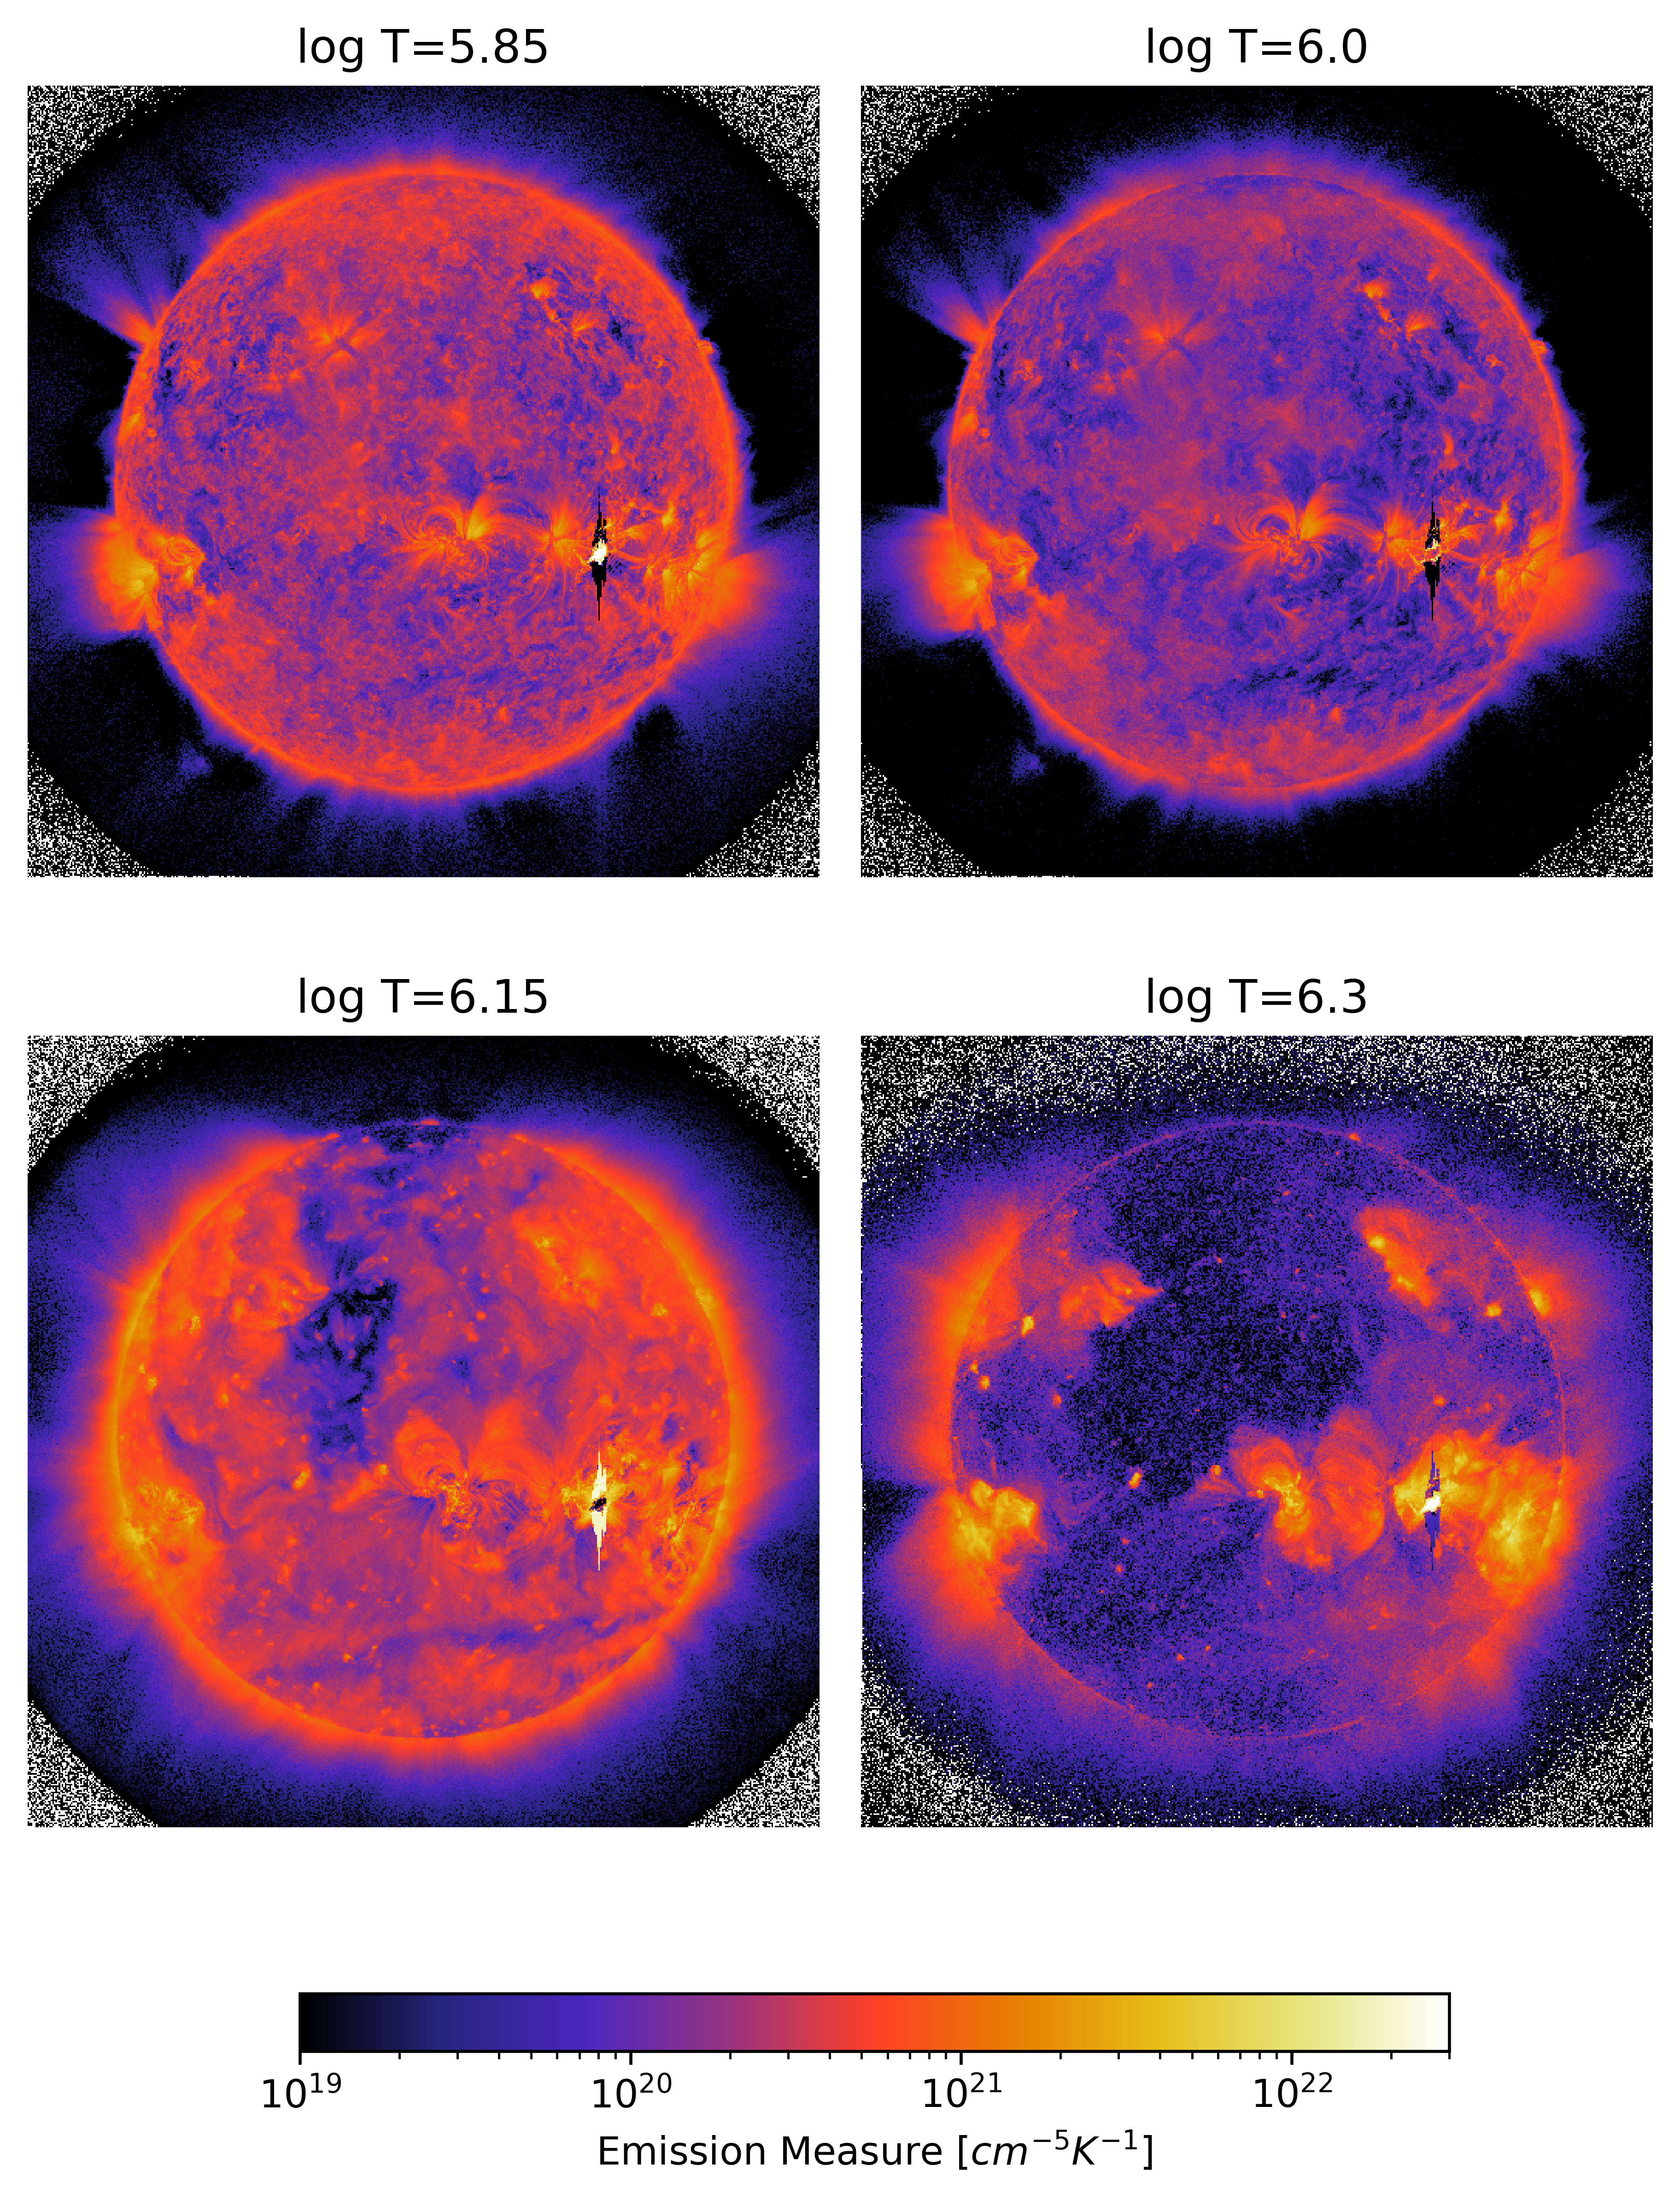
\includegraphics[width=0.5\textwidth]{images/dem_img_aug_4_2011.png}
    \caption[DEM full disk image of Sun]{DEM of Sun during the flaring event on \nth{4} August 2011. The artifacts at the corners of the image is due to the diffraction of light in the telescope of AIA}
    \label{fig:dem_img_aug_4_2011}
\end{figure}

Next step is to generate the point source from the full disk, which we refer to as ``Pointification''. This involves the conversion of the full disk image of Sun to a point source, which mimics a distant star. The original image of 4096 $\times$ 4096 pixels dimension is averaged and new image having 512 $\times$ 512 pixels dimension is created with the pixel value at (256, 256) of the image (midpoint of the image) equal to the calculated average image pixel value. The average values of 4096 $\times$ 4096 pixel image dimension has been considered and not the 512 one so as to not allow the errors due to the resampling of the image affect the average pixel intensity value significantly. \Cref{fig:ps_plus_full_disk} shows the result of pointification procedure. After pointification, DEM profile is reconstructed from these images. These act like DEM profiles of a point source/star.\\

\begin{figure}[h!]
    \centering
    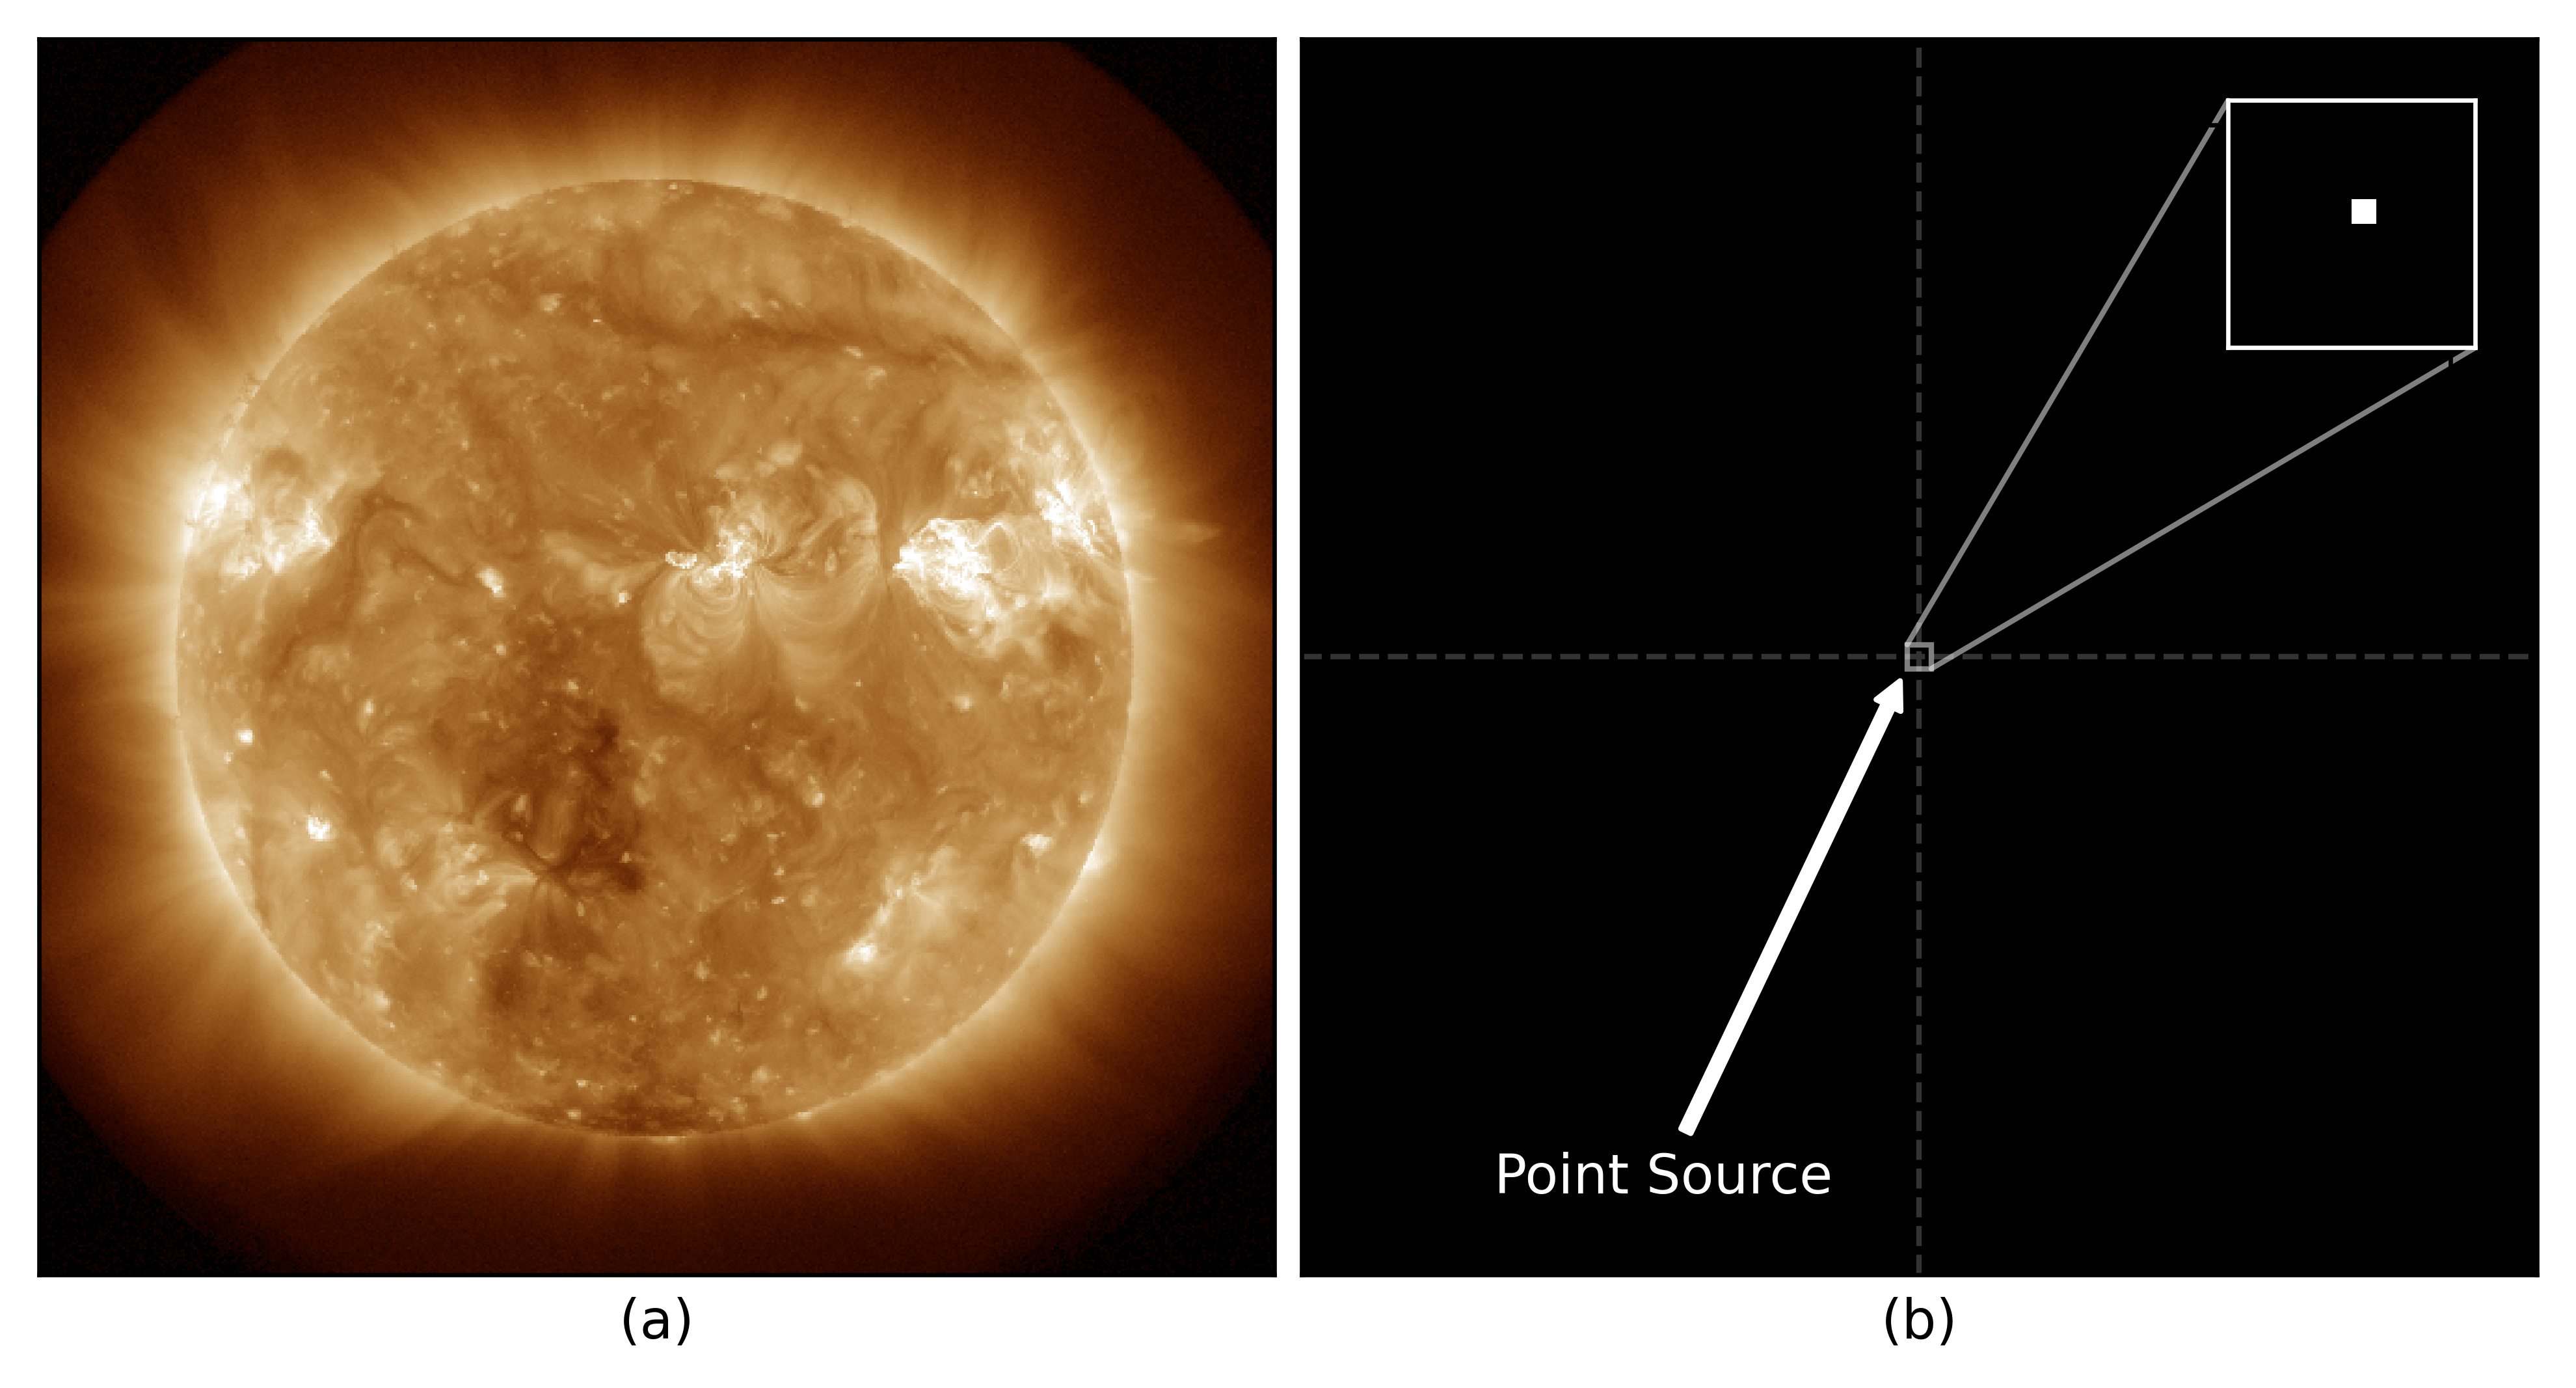
\includegraphics[width=0.95\textwidth]{images/ps_plus_full_disk.png}
    \caption[Full disk and pointified image of Sun]{\textbf{(a)} shows the full disk image of Sun in the 193 $\AA$ channel, \textbf{(b)} shows the image after pointification.}
    \label{fig:ps_plus_full_disk}
\end{figure}

The temperature logT can be grouped into discrete ranges with the corresponding dem solutions being group by averaging. The grouping interval depends on the temperature interval used for the analysis, which in our case is 0.15 K. We have grouped three consecutive temperature intervals (eg: 5.85, 6.0, 6.15). This is called as temperature binning. Binning helps in reducing the impact of noise or uncertainities in the data. By averaging the emission measuresments for each temperature bin, we can smoothen fluctuations and obtain a good estimate of the DEM.

%%% Local Variables:
%%% mode: LaTeX
%%% TeX-master: "main"
%%% End:


\section{Results}

\Cref{fig:dem_ts_aug_04_2011}, \cref{fig:dem_ts_aug_31_2012} and \cref{fig:dem_ts_oct_28_2021} shows the timeseries plot of DEM for the three events. The time series plot is calculated by averaging the acceptable DEM solutions obtained for each image over three consecutive temperature range (i.e averaging the solutions for 5.85, 5.9 and 5.95 etc.). Blue curve corresponds to the full disk DEM and red curve corresponds to the point source DEM. The temperature range above logT=6.75 has been omitted as no correlation was found between point source and full disk.

\begin{figure}[h!]
    \centering
    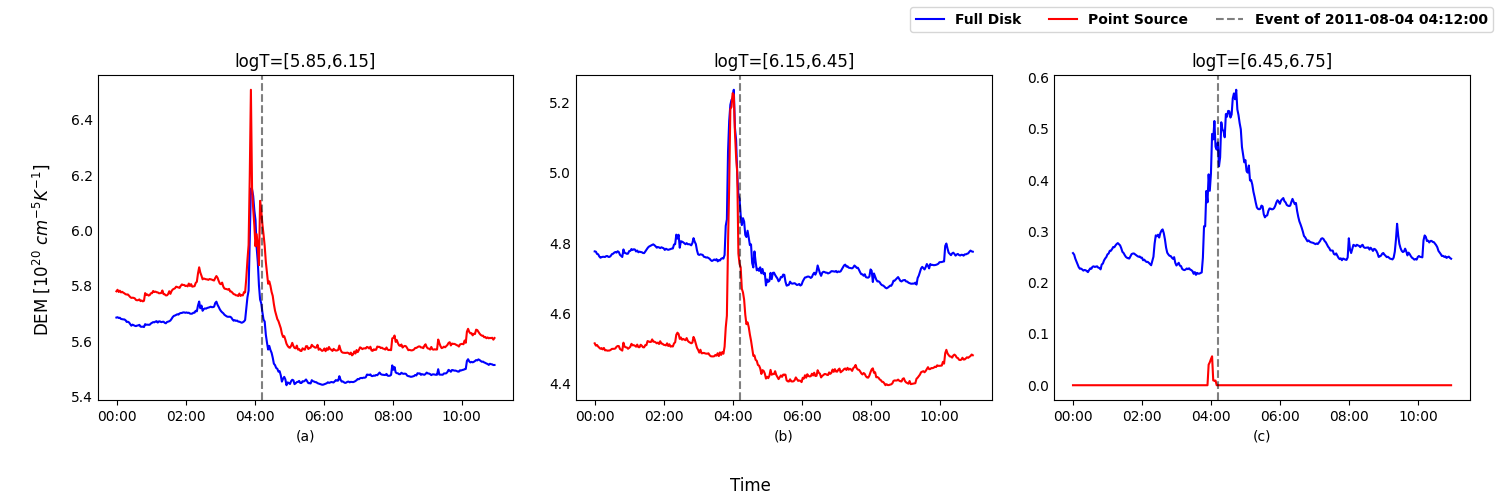
\includegraphics[width=\textwidth]{images/dem_ts_aug_04_2011.png}
    \caption[DEM Timeseries for August 2011 Event]{Timeseries of DEM for \nth{4} August 2011 Event.}
    \label{fig:dem_ts_aug_04_2011}
\end{figure}

\begin{figure}[h!]
    \centering
    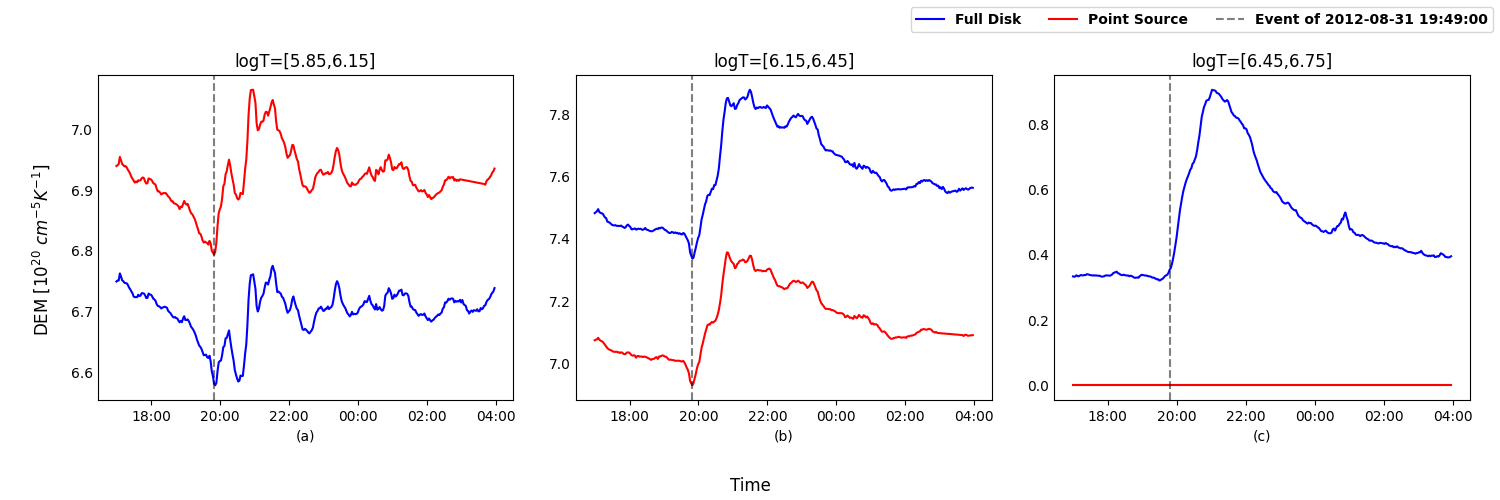
\includegraphics[width=\textwidth]{images/dem_ts_aug_31_2012.png}
    \caption[DEM Timeseries for August 2012 Event]{Timeseries of DEM for \nth{31} August 2012 Event}
    \label{fig:dem_ts_aug_31_2012}
\end{figure}

\begin{figure}[h!]
    \centering
    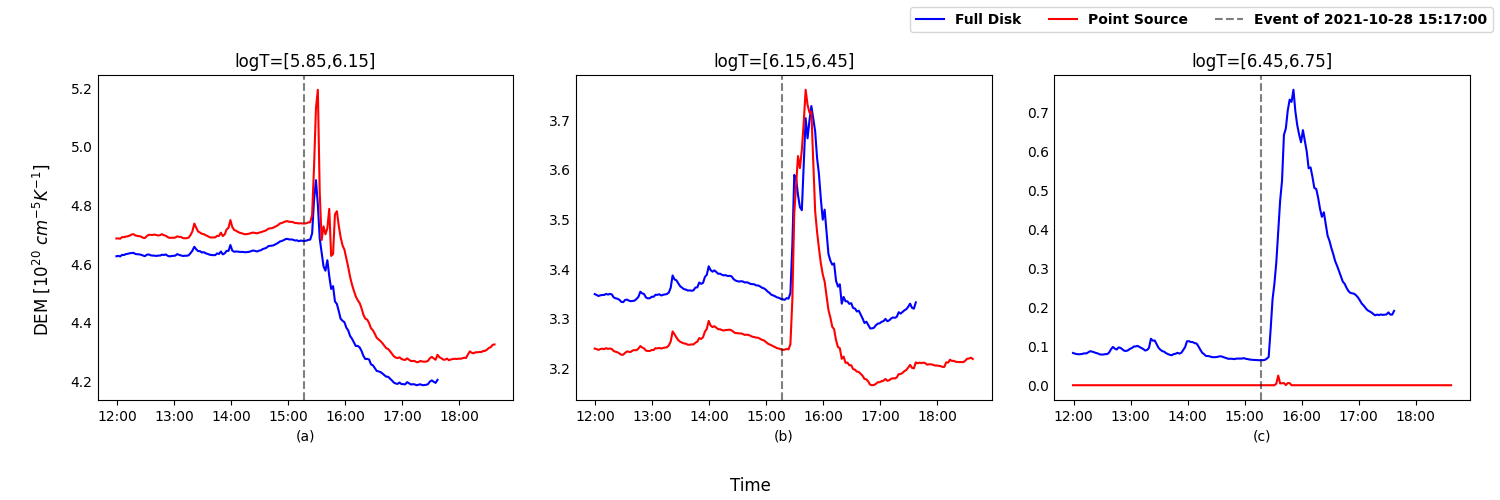
\includegraphics[width=\textwidth]{images/dem_ts_oct_28_2021.png}
    \caption[DEM Timeseries for October 2021 Event]{Timeseries of DEM for \nth{28} October 2021 Event}
    \label{fig:dem_ts_oct_28_2021}
\end{figure}

In \cref{fig:dem_ts_aug_04_2011}(a) and \cref{fig:dem_ts_aug_04_2011}(b), we can observe the coronal dimming or decrease in the DEM value after the event spike. But, in \cref{fig:dem_ts_aug_04_2011}(c) no dimming is observed. Dimming is the most prominent in logT = [5.85, 6.15]. The sudden increase in the DEM curve is due to the solar flare which is associated with the CME. There is very high correlation for the first two temperature ranges, but there is little to no correlation in the DEM profiles of the full disk and point source for the temperature range logT=[6.45, 6.75]. For temperature ranges greater than logT=6.45, the correlation is almost 0. We make use of Pearson's Correlation coeffecient (\cref{eqn:pearsonr}) to find out the amount of correlation between the point source and full disk DEM, for which we use \texttt{pearsonr} function from the \texttt{scipy} library in Python. The pearson correlation coeffecient r between two datasets \textbf{x} and \textbf{y} is calculated using the formula,

\begin{equation}
    \label{eqn:pearsonr}
    r = \frac{\sum (x_i - \overline{x})(y_i - \overline{y})}{\sqrt{\sum (x_i - \overline{x})^2 \sum (y_i - \overline{y})^2}}
\end{equation}\hspace{0.25cm}

\begin{table}[h!]
    \centering
    \begin{tblr}{
          cell{1}{1} = {r=2}{},
          cell{1}{2} = {c=3}{c},
          vline{1-5} = {-}{},
          hline{1-6} = {-}{},
        }
        \textbf{Event} & \textbf{Pearson Correlation Coeffecient} &         & \\
        & logT=[5.85, 6.15]  & logT=[6.15, 6.45] & logT=[6.45, 6.75] \\
        \nth{4} August 2011  & 0.9449 & 0.9767 & 0.2190\\
        \nth{31} August 2012  & 0.7027 & 0.9885 & 0.2079\\
        \nth{28} October 2021 & 0.9555 & 0.9577 & 0.2578 \\
    \end{tblr}
    \caption{Correlation between Point source and Full Disk DEM}
\end{table}

We see a discrepancy in the value of DEM between the point source and full disk average values. This could be due to the error induced during the DEM profile reconstruction, instrumental errors, error incurred during the resampling or reduction of image dimension from 4096 $\times$ 4096 pixels to 512 $\times$ 512 and it could also be due to averaging error. The dataset length is not equal in some of the case as invalid or small DEM solution values have been removed.\\

The temperature distribution of the plasma at different sections of an event can be studied through it's DEM profile (DEM profile is a plot of logT vs DEM). The DEM profiles before, during and after the event has been shown in \cref{fig:dem_pro_aug_04_2011}, \cref{fig:dem_pro_aug_31_2012} and \cref{fig:dem_pro_oct_28_2021} for the events of \nth{4} August 2011, \nth{31} August 2012 and \nth{28} October 2021 respectively.

\begin{figure}[h!]

    \begin{subfigure}[b]{0.3\textwidth}
        \centering
        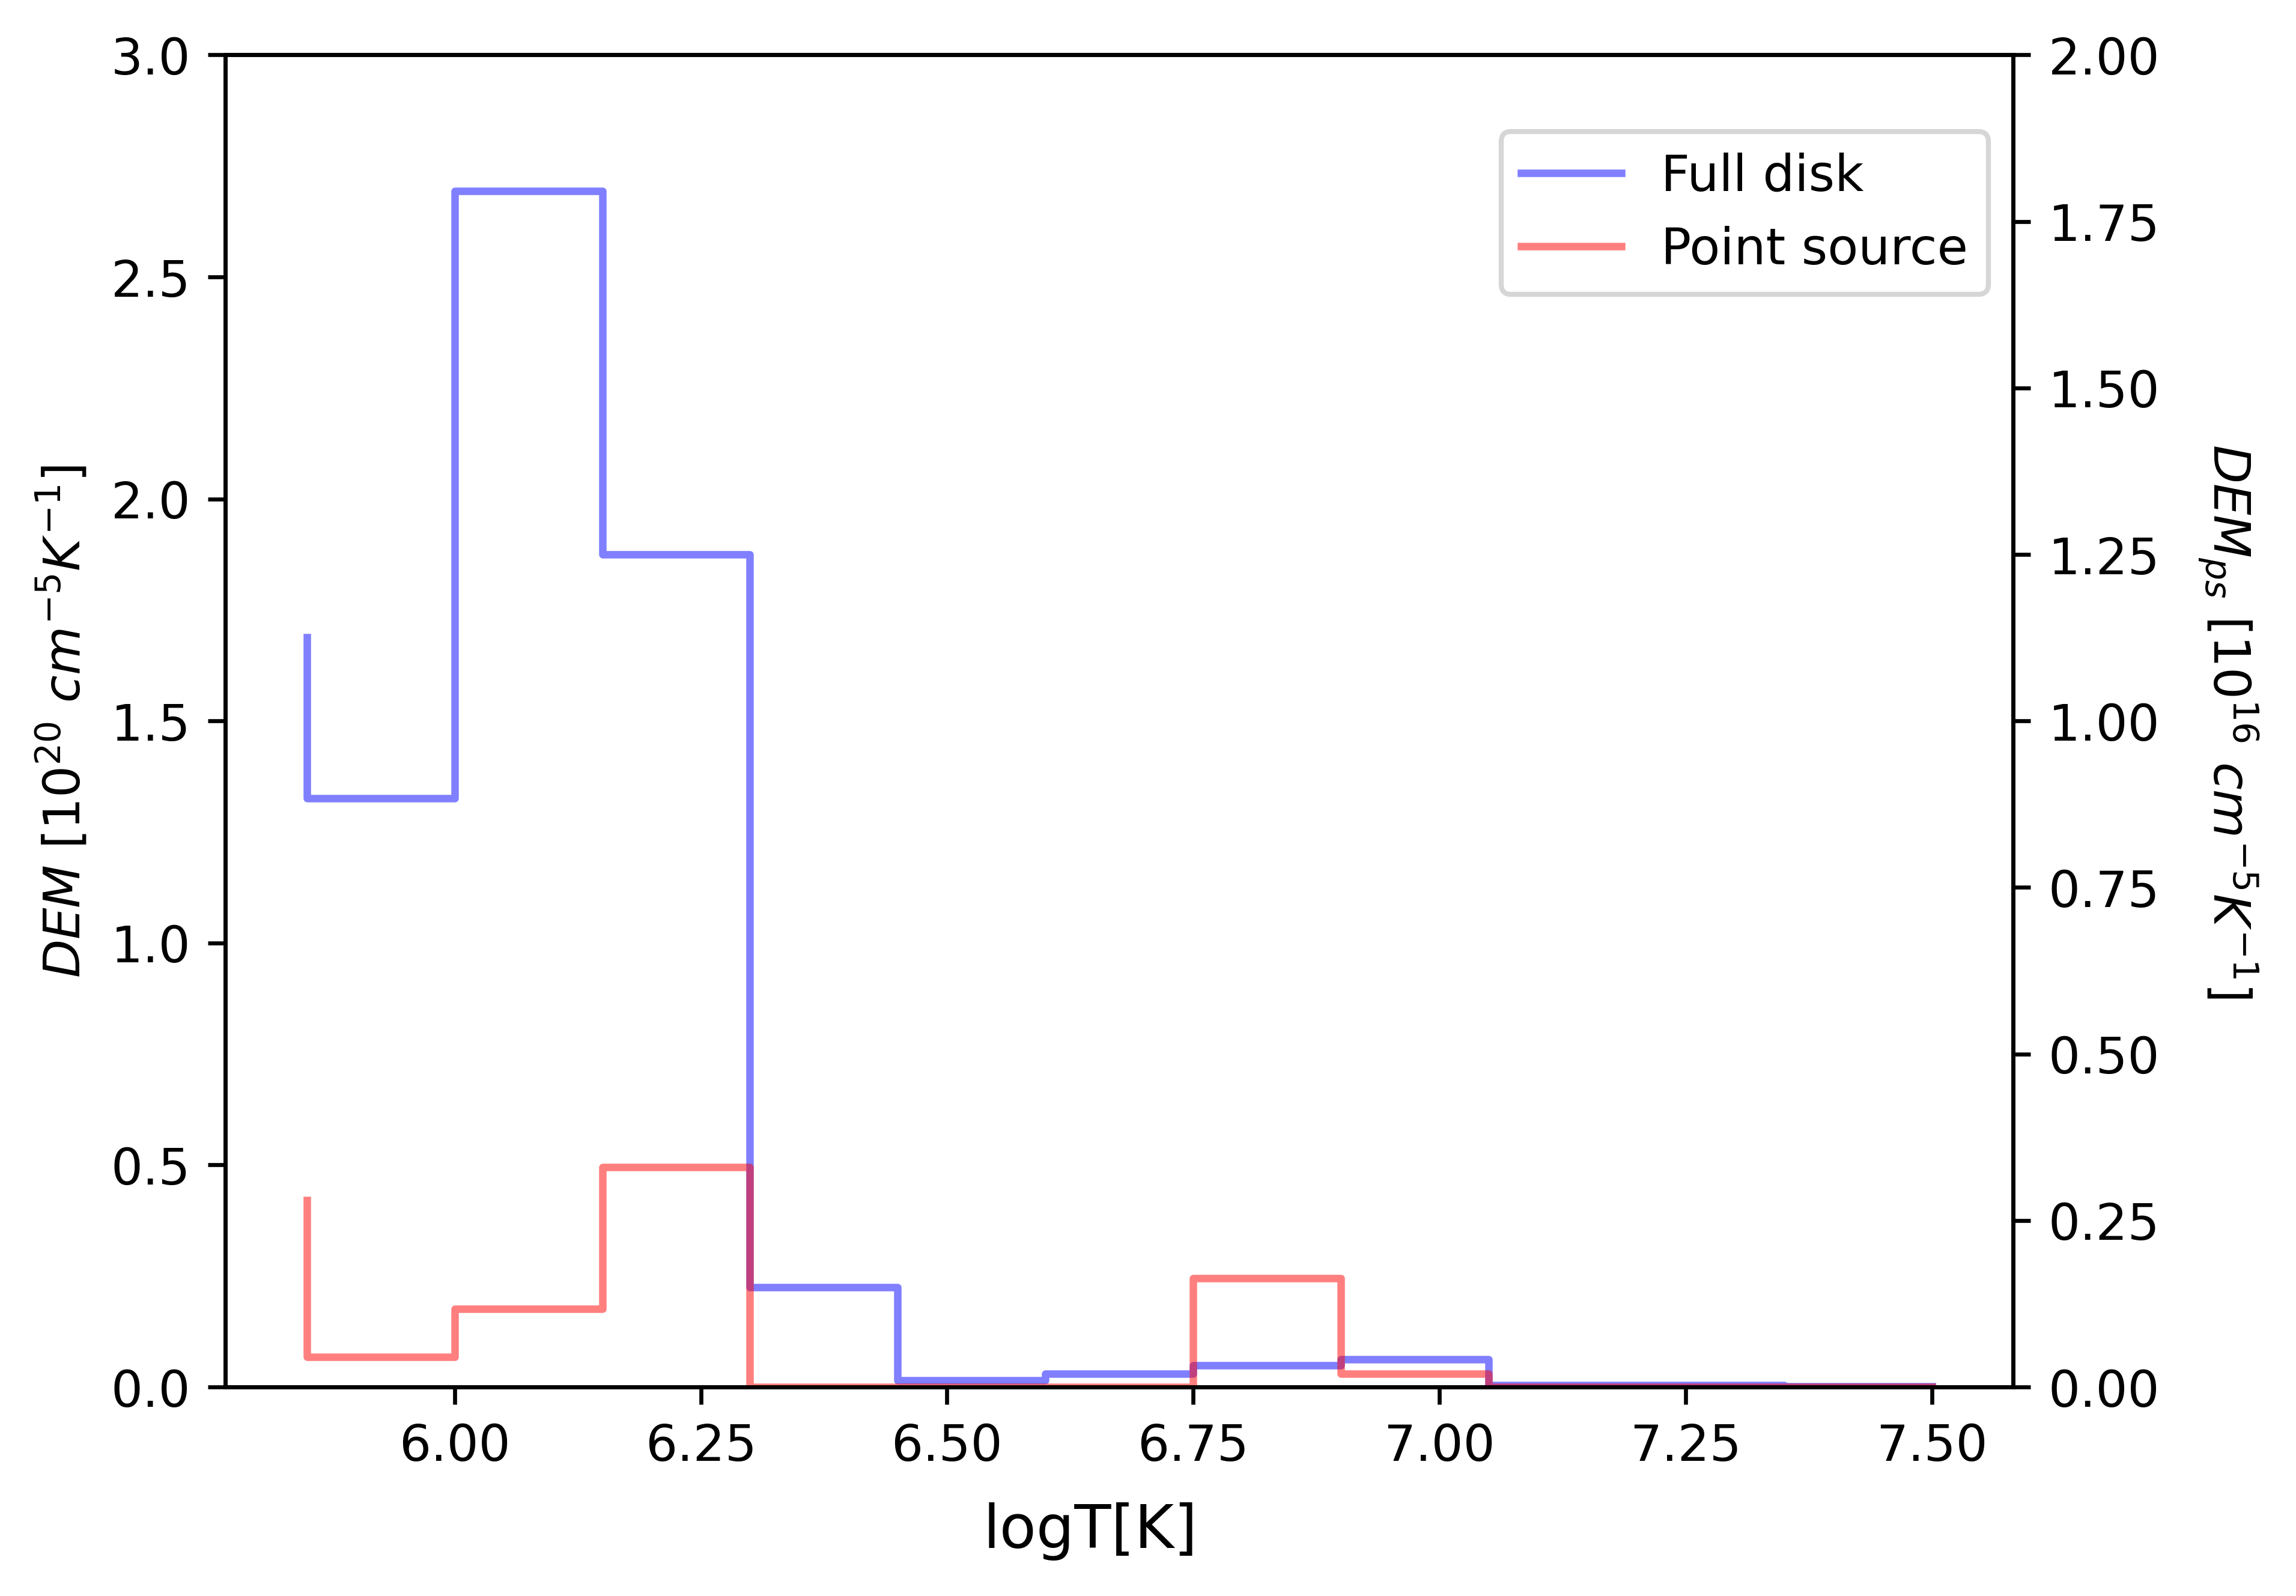
\includegraphics[width=\textwidth]{images/dem_profile_before_event_2011_aug_04.png}
        \caption{Before event (02:21 UT)}
    \end{subfigure}
    \hfill
    \begin{subfigure}[b]{0.3\textwidth}
        \centering
        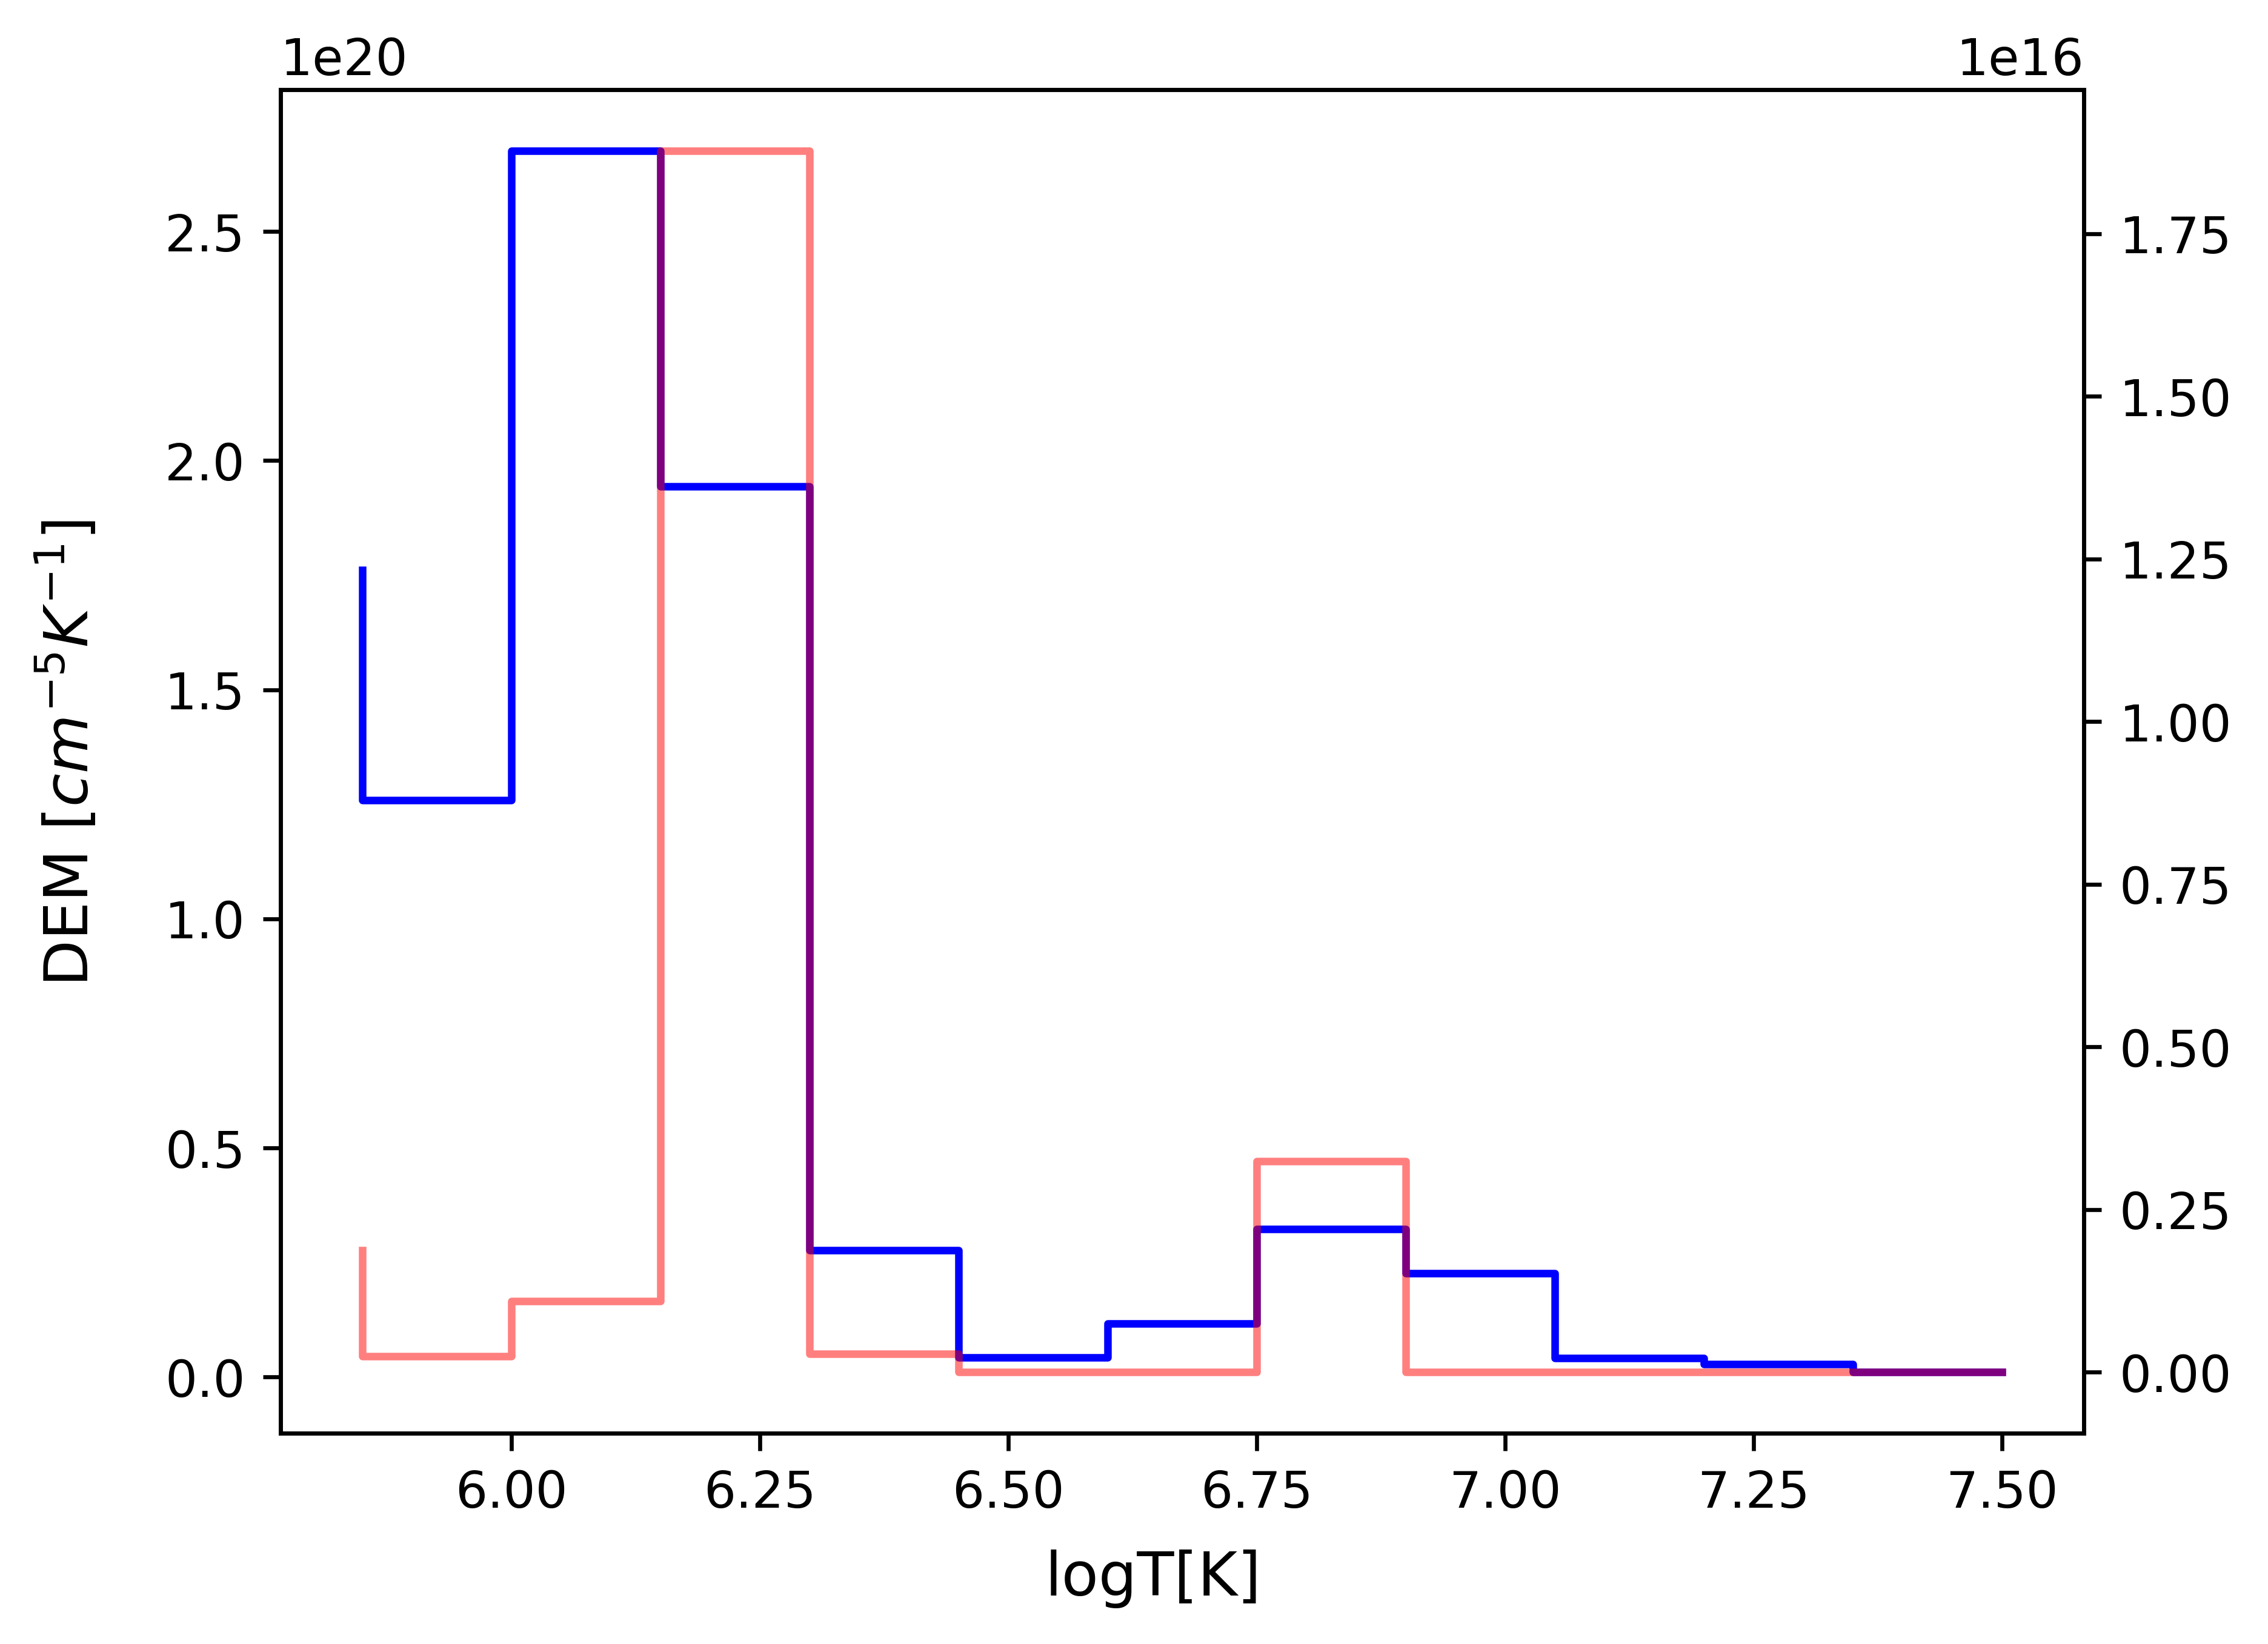
\includegraphics[width=\textwidth]{images/dem_profile_during_event_2011_aug_04.png}
        \caption{During event (04:11 UT)}
    \end{subfigure}
    \hfill
    \begin{subfigure}[b]{0.3\textwidth}
        \centering
        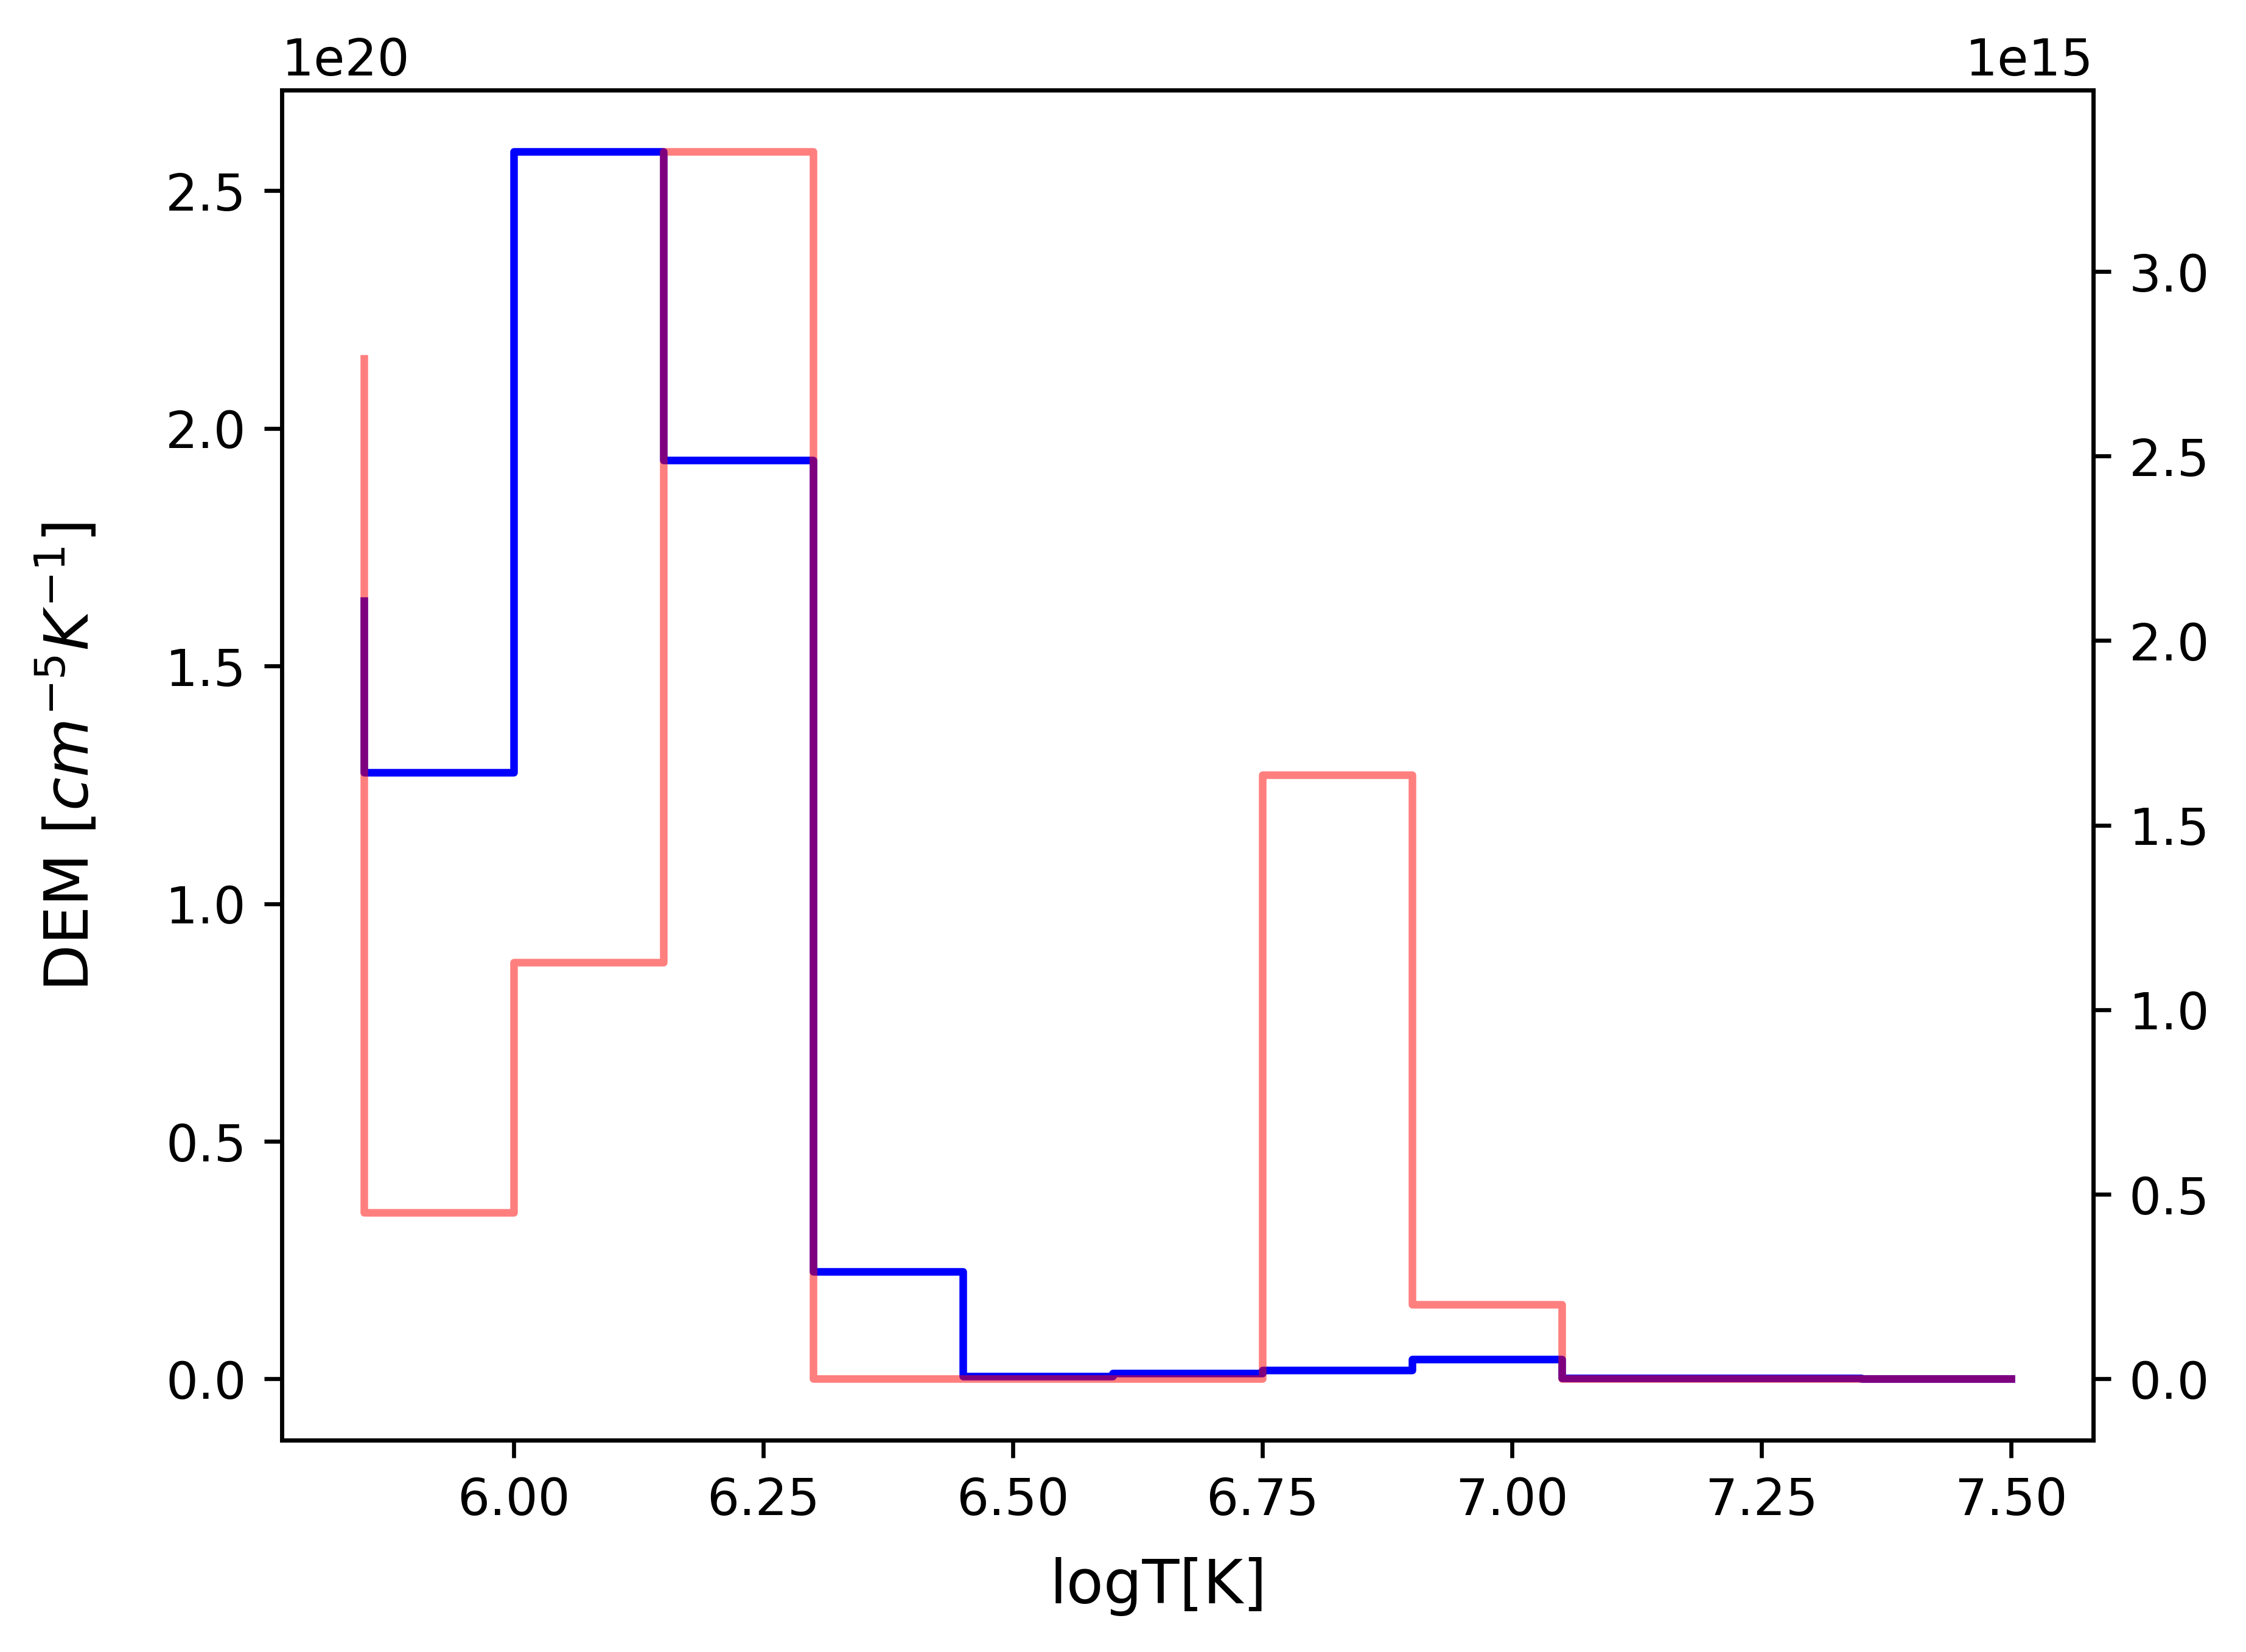
\includegraphics[width=\textwidth]{images/dem_profile_after_event_2011_aug_04.png}
        \caption{After event (10:49 UT)}
    \end{subfigure}

    \caption[DEM profile for \nth{4} August 2011 event]{DEM profile before, during and after the flaring event of \nth{4} August 2011. The red and blue curves correspond to point source and full disk source respectively.}
    \label{fig:dem_pro_aug_04_2011}
\end{figure}


\begin{figure}[h!]

    \begin{subfigure}[b]{0.3\textwidth}
        \centering
        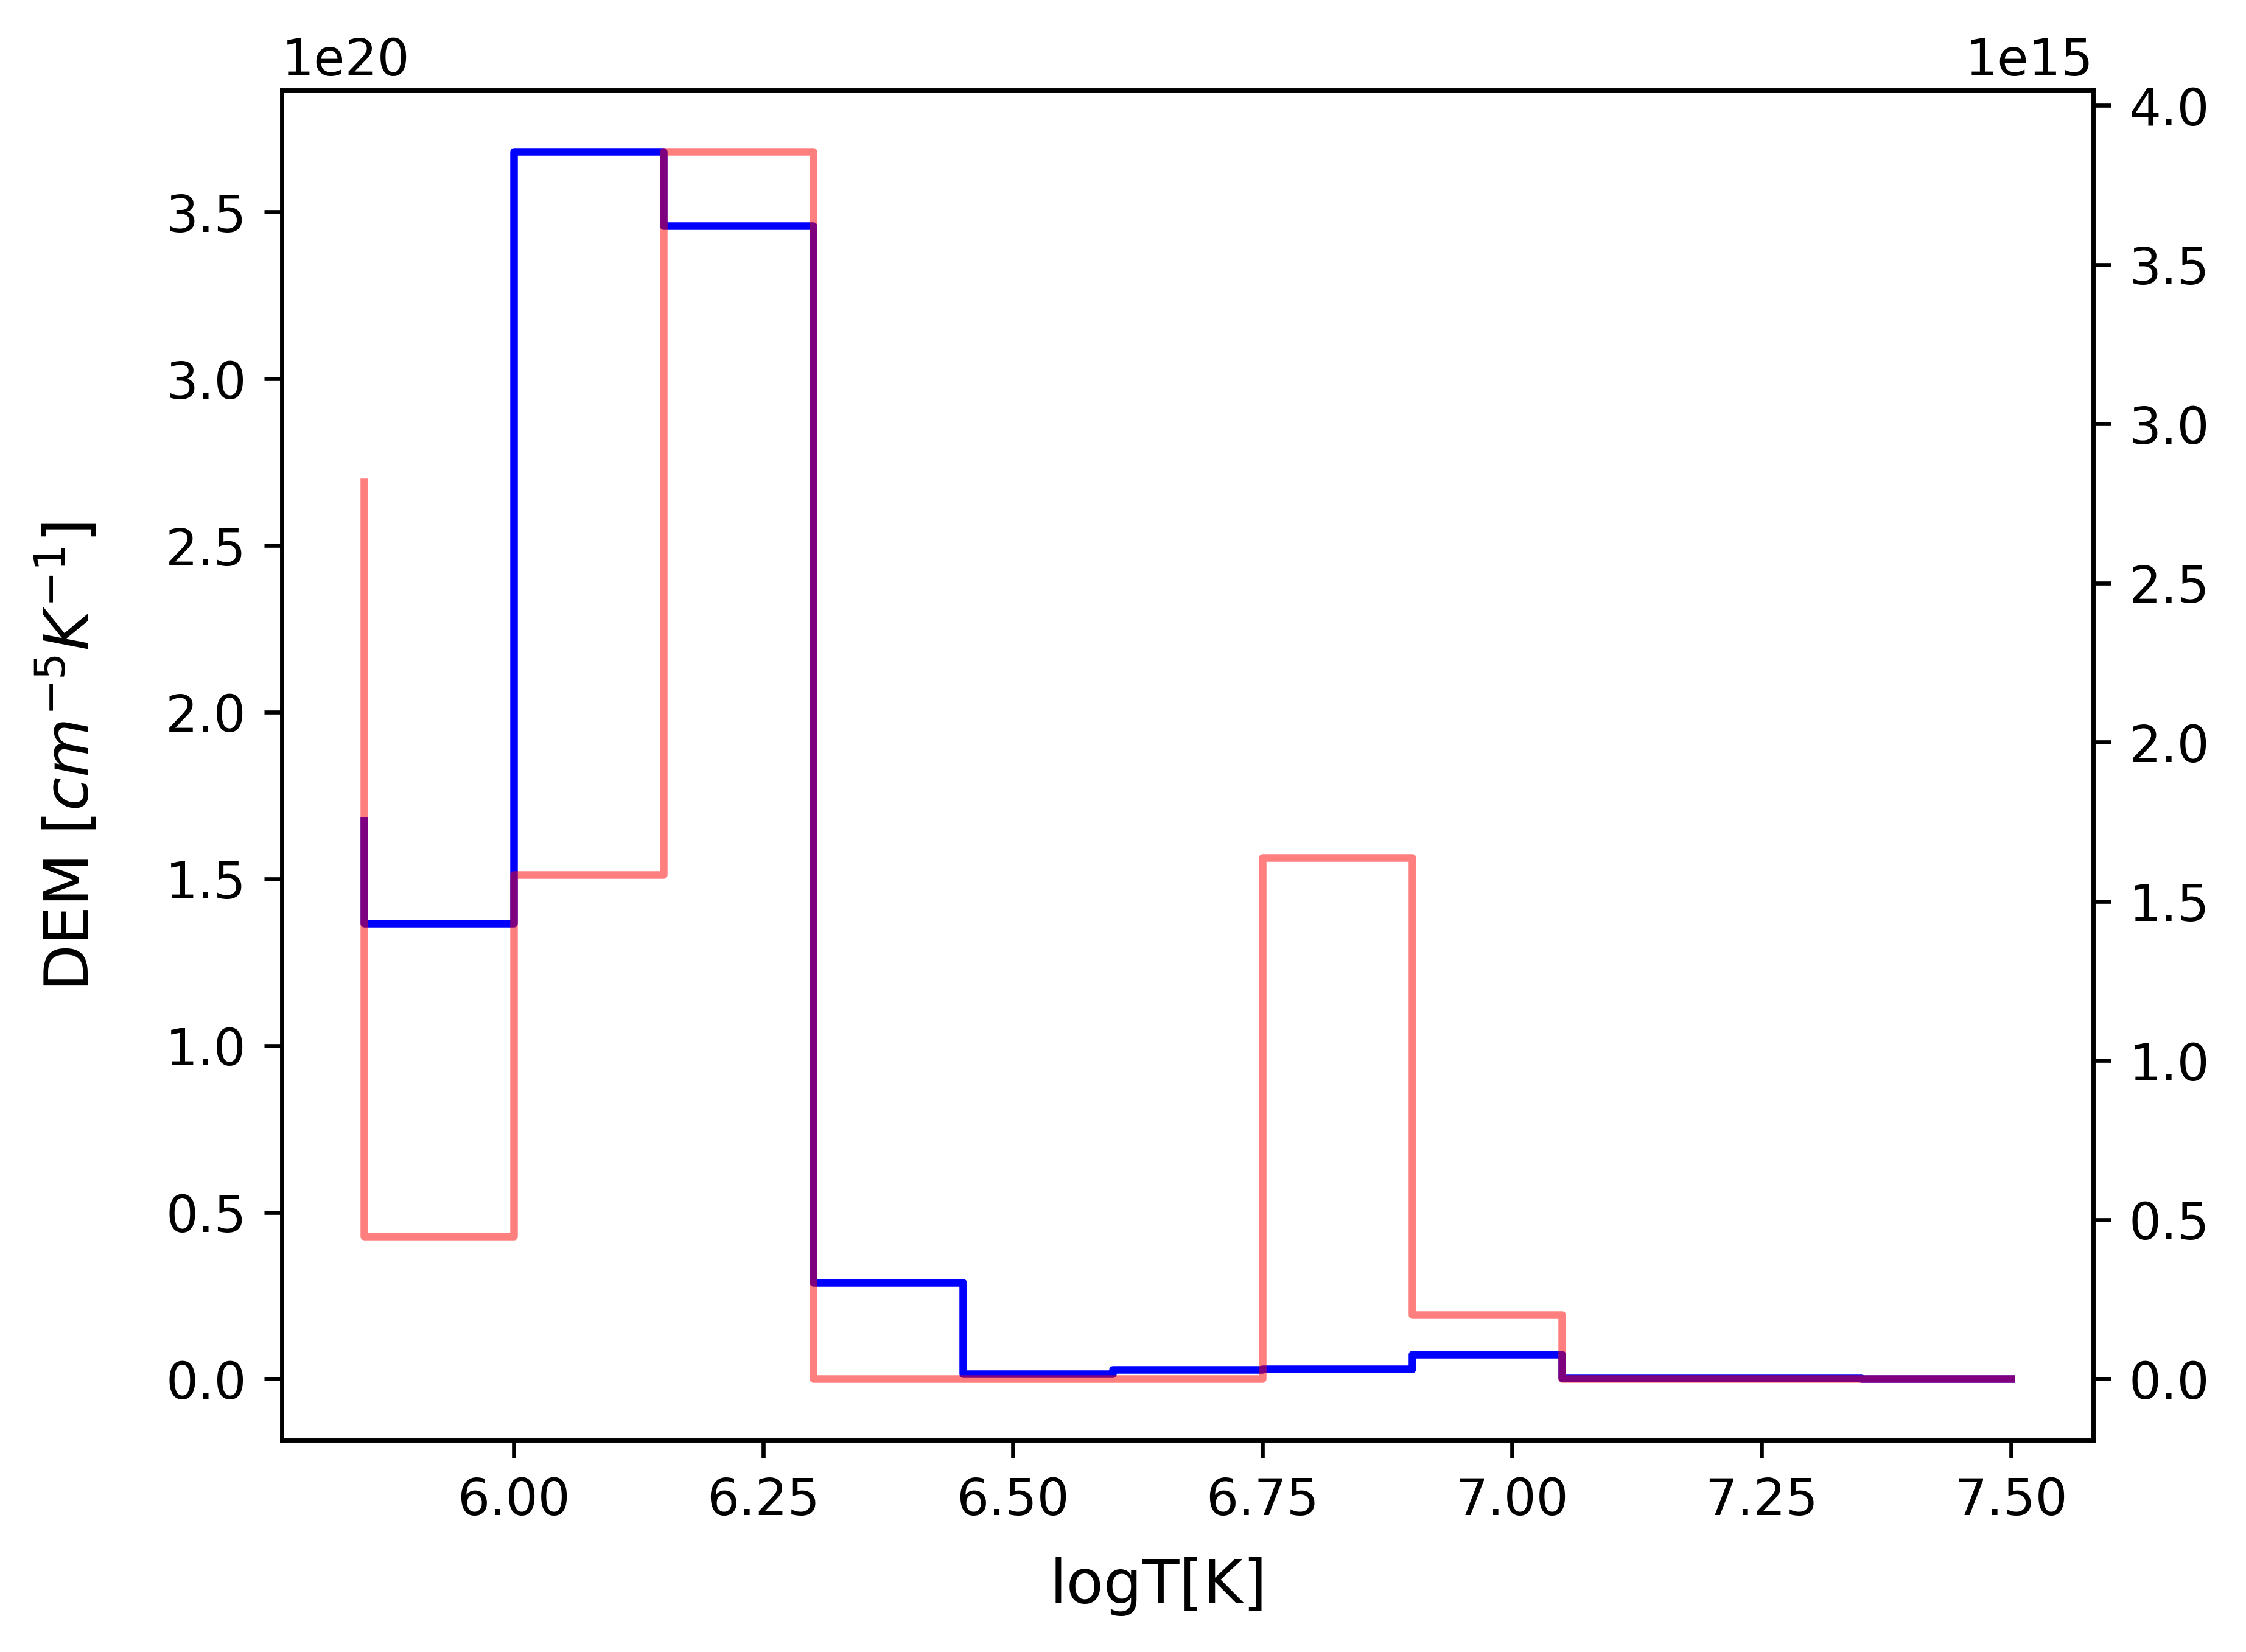
\includegraphics[width=\textwidth]{images/dem_profile_before_event_2012_aug_31.png}
        \caption{Before event (17:19 UT)}
    \end{subfigure}
    \hfill
    \begin{subfigure}[b]{0.3\textwidth}
        \centering
        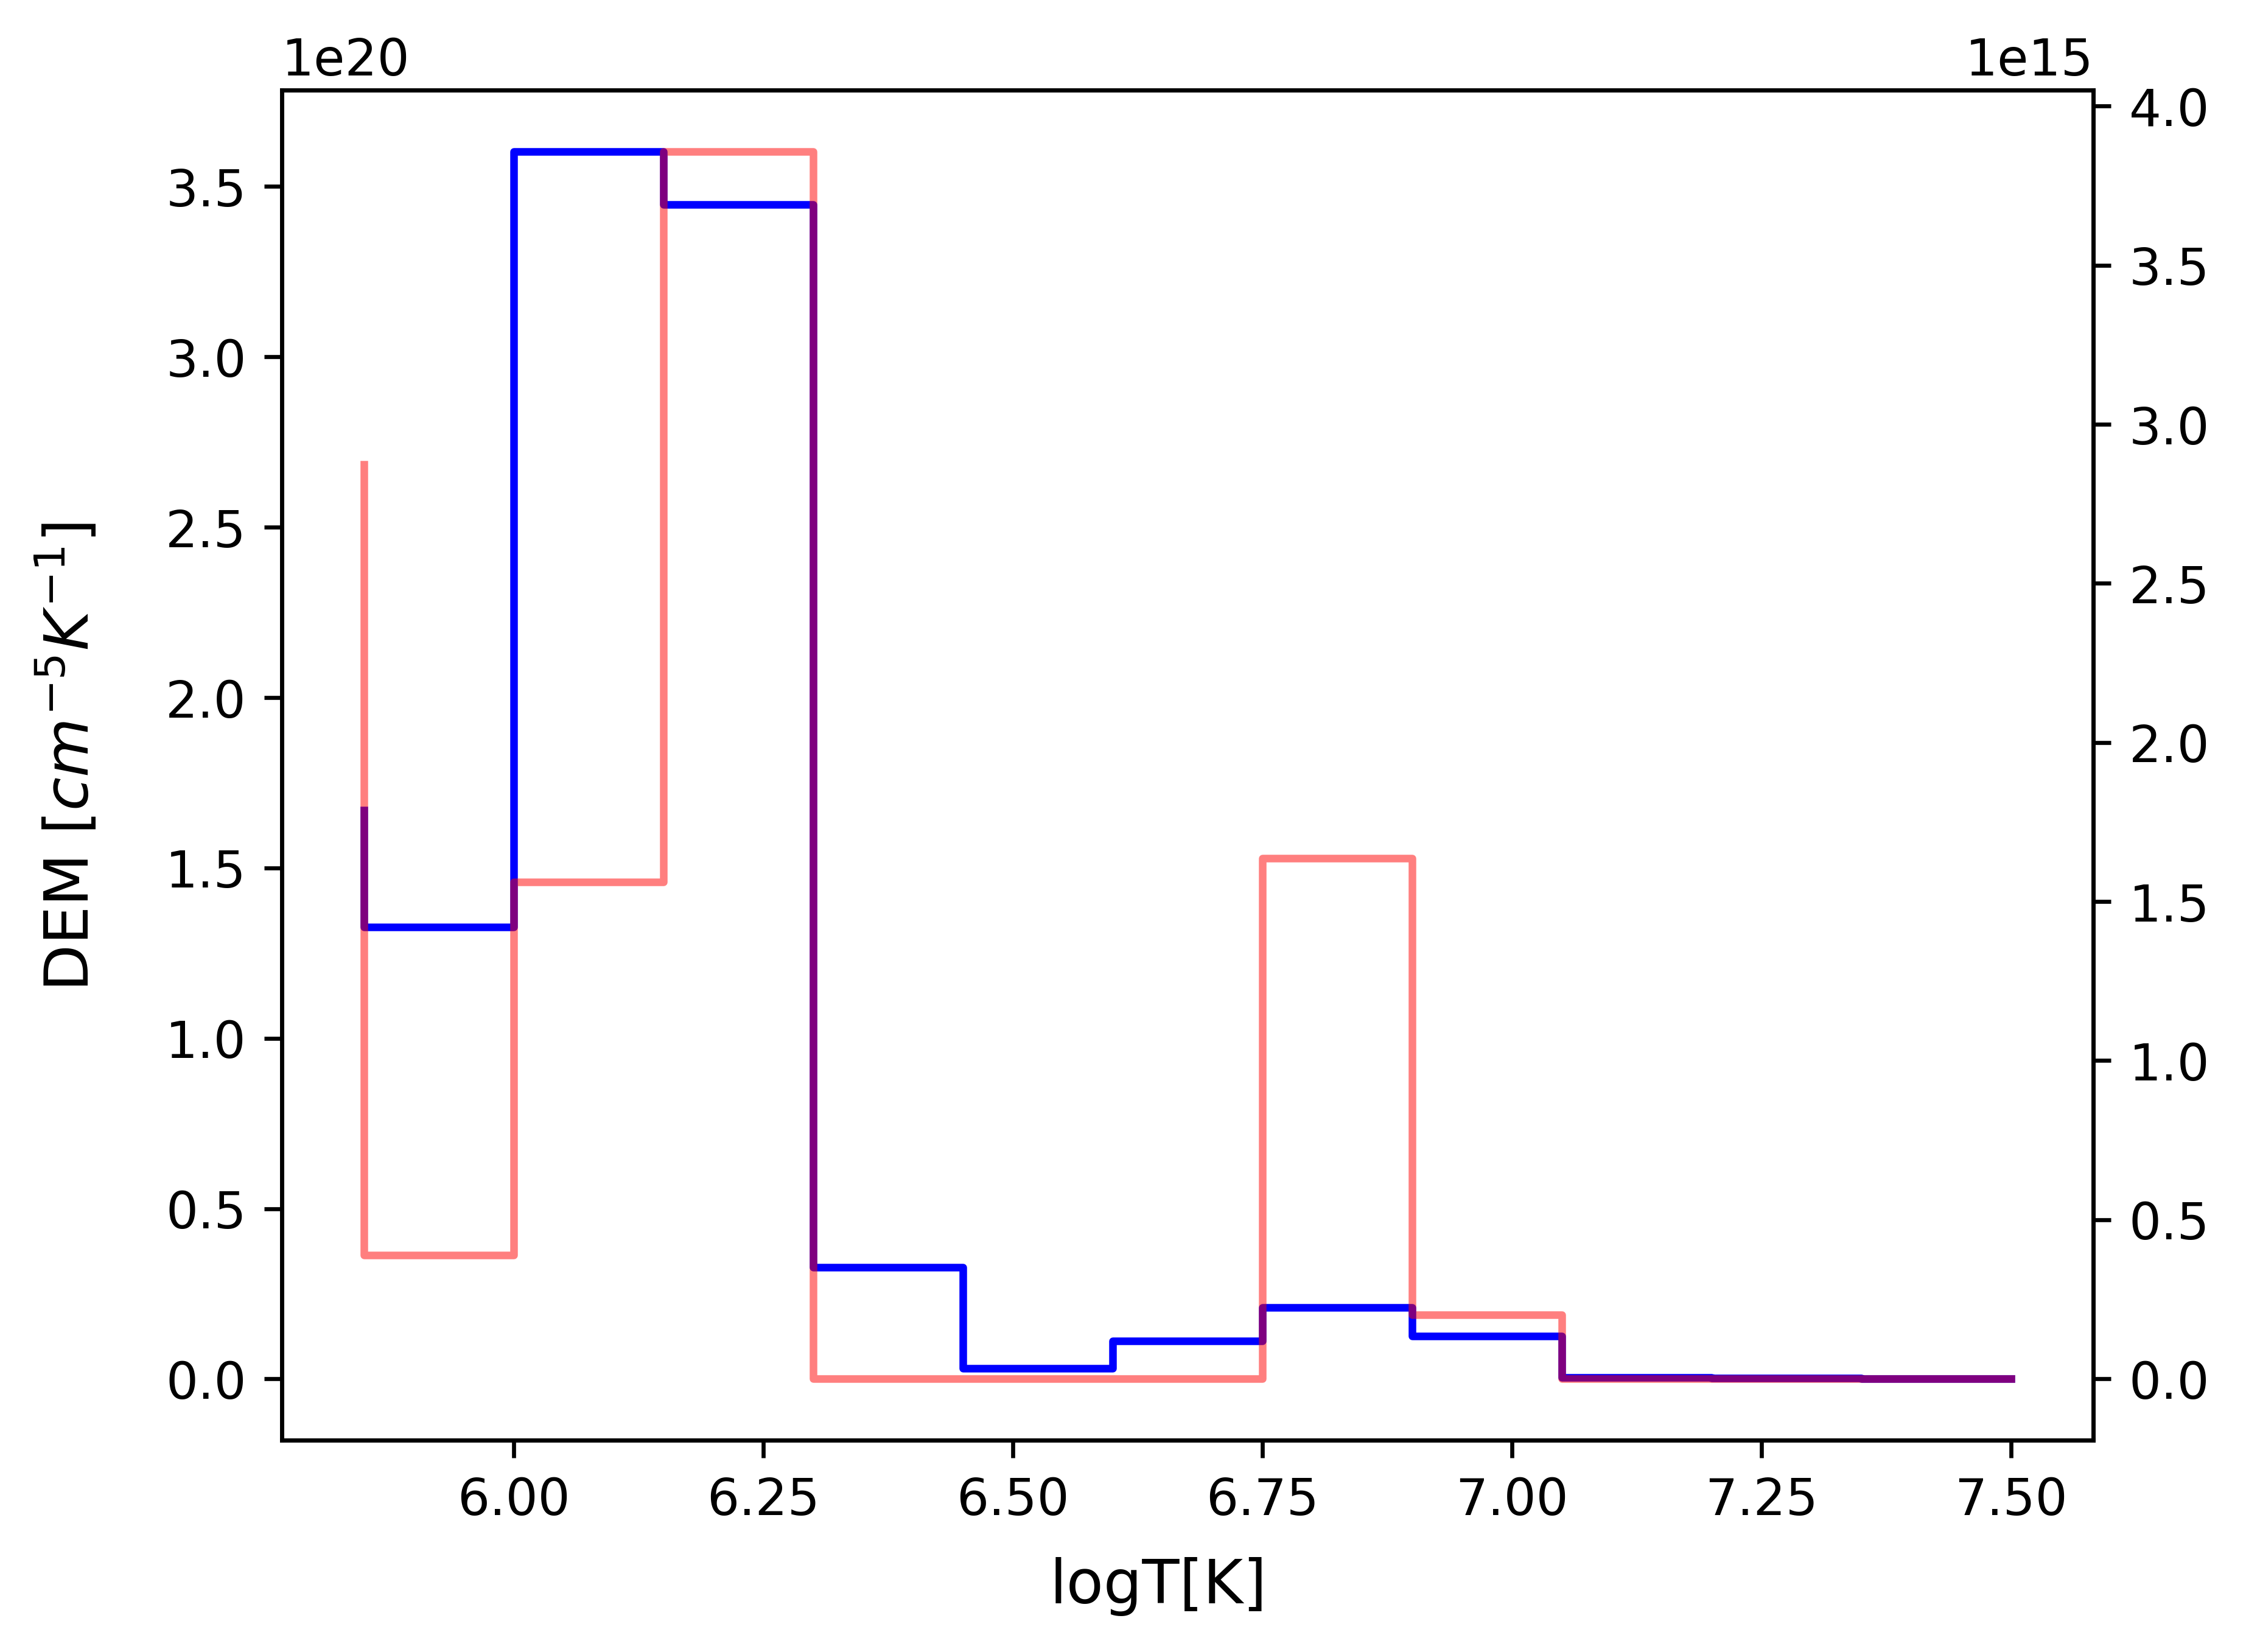
\includegraphics[width=\textwidth]{images/dem_profile_during_event_2012_aug_31.png}
        \caption{During event (20:01 UT)}
    \end{subfigure}
    \hfill
    \begin{subfigure}[b]{0.3\textwidth}
        \centering
        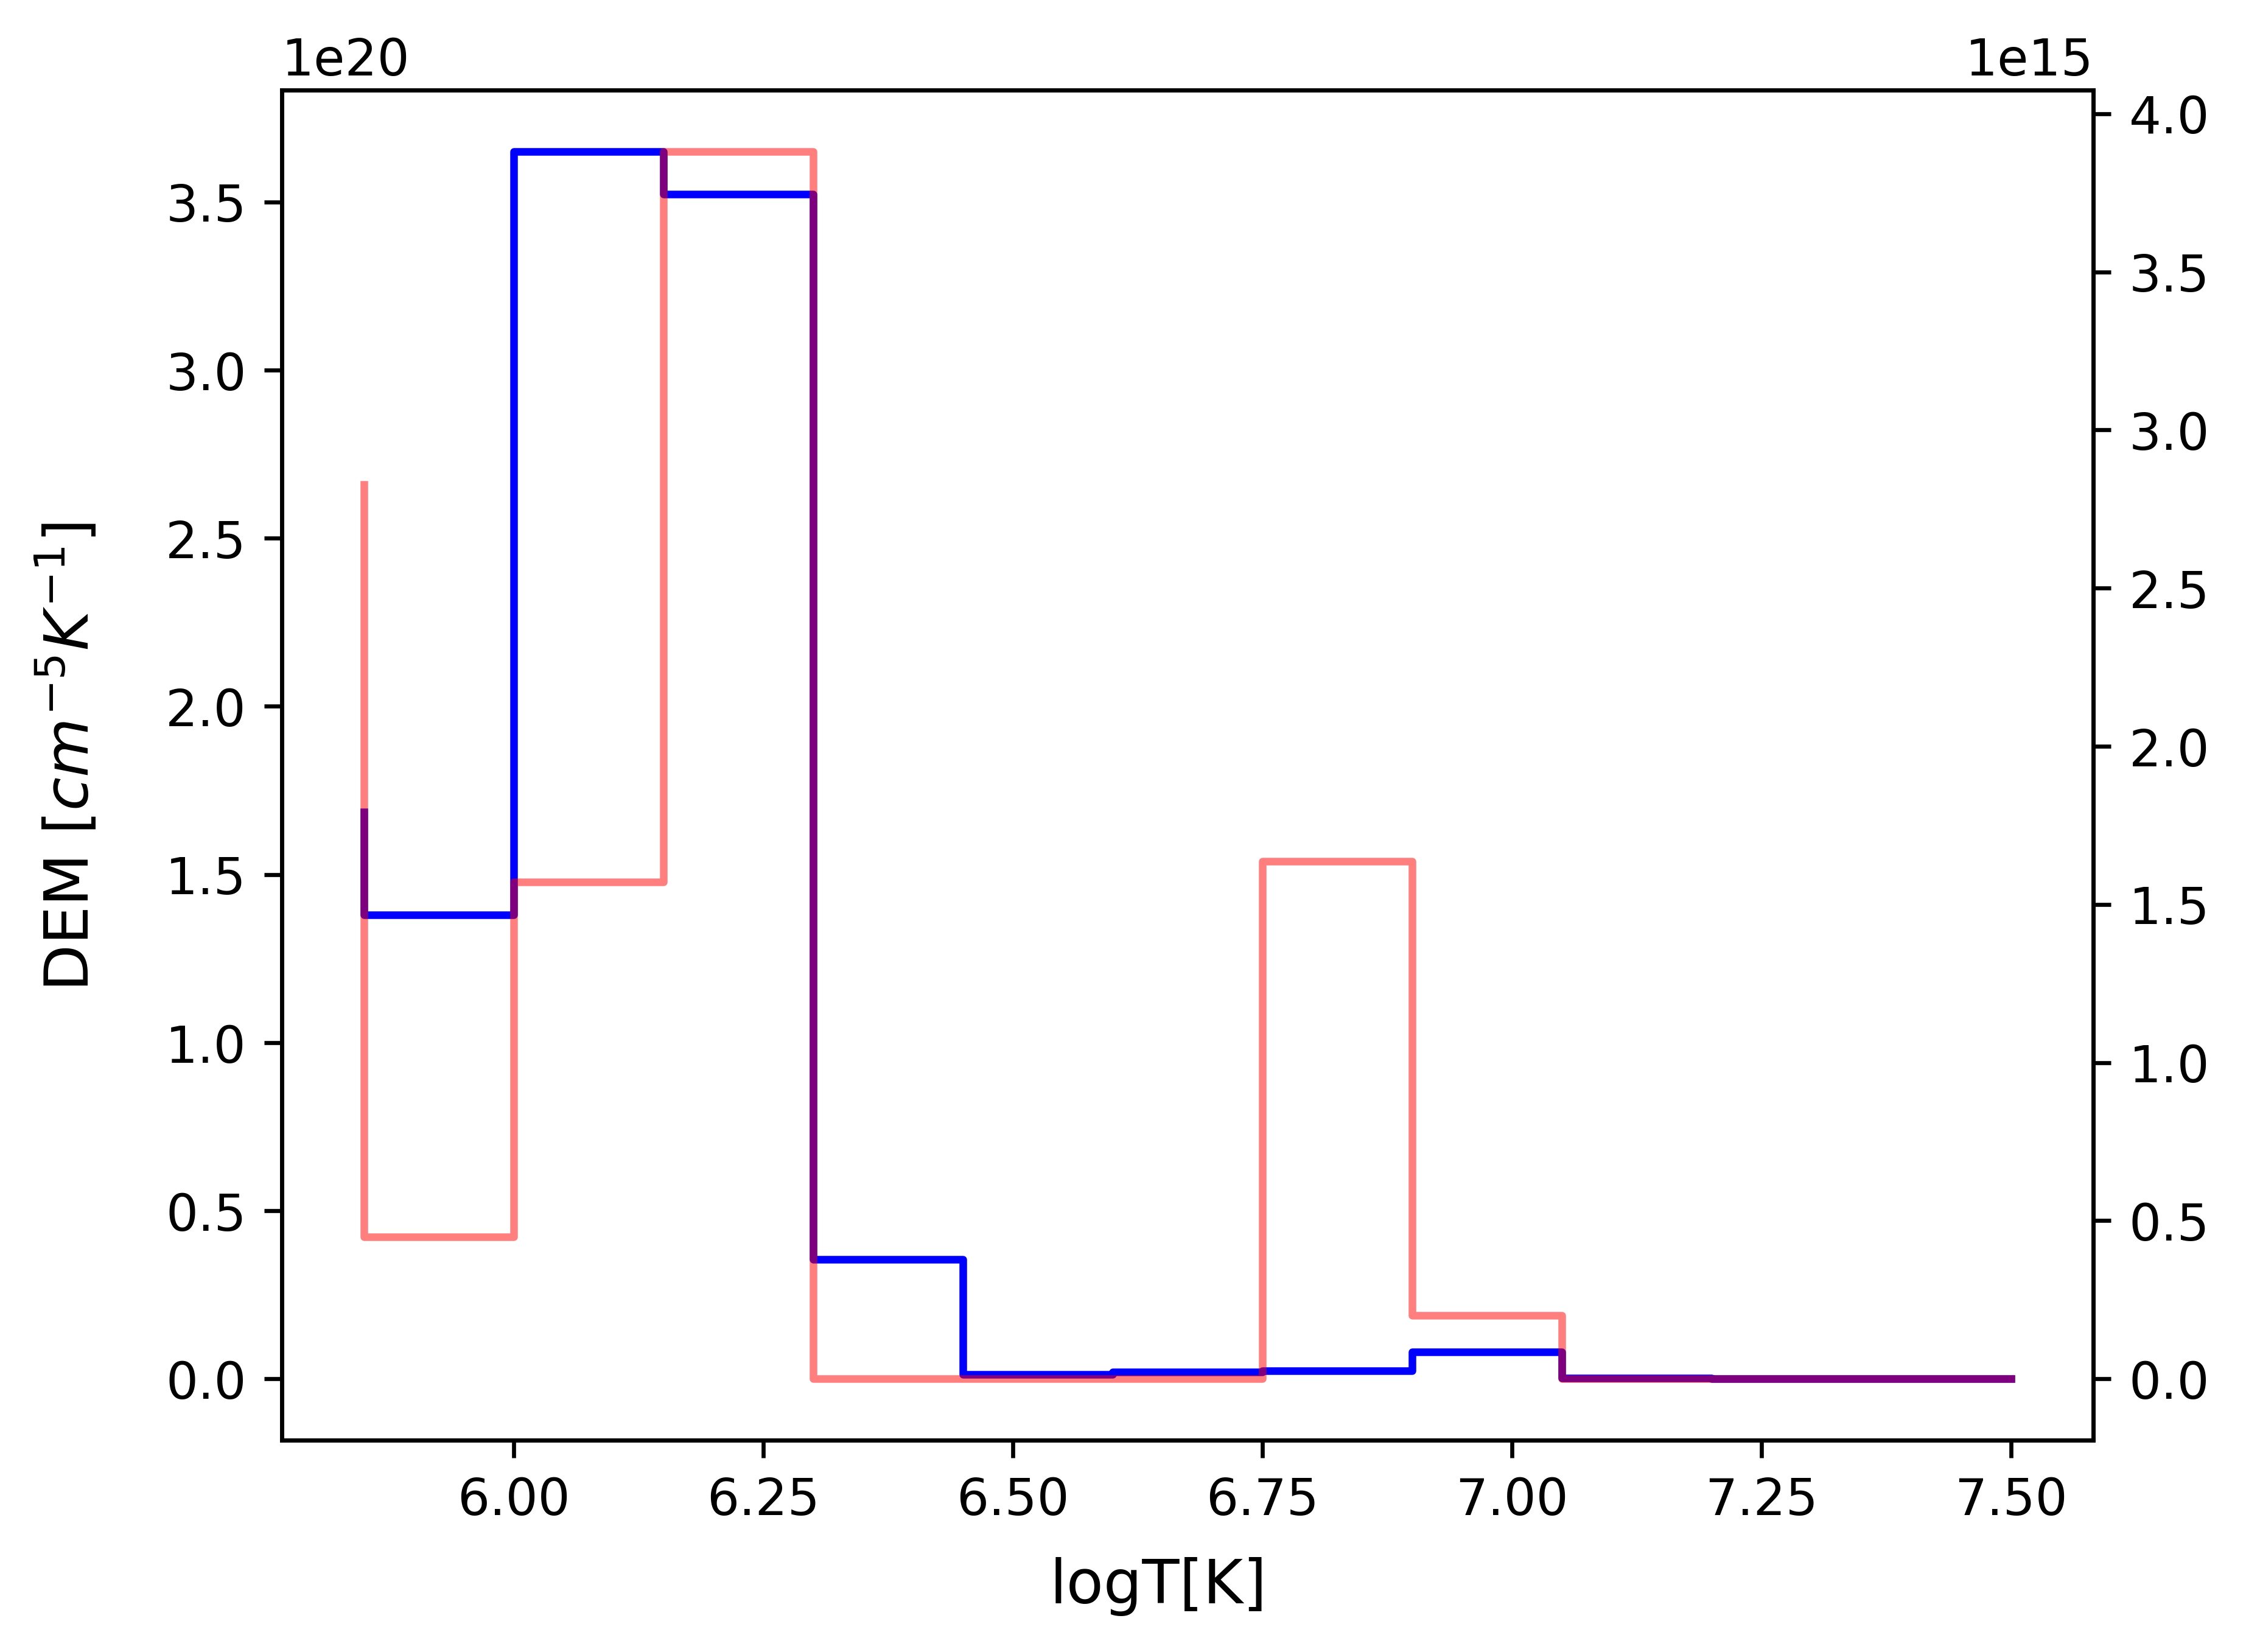
\includegraphics[width=\textwidth]{images/dem_profile_after_event_2012_aug_31.png}
        \caption{After event (\nth{1} September 2011 03:57 UT)}
    \end{subfigure}

    \caption[DEM profile for \nth{31} August 2012 Event]{DEM profile before, during and after the flaring event of \nth{31} August 2012. The red and blue curves correspond to point source and full disk source respectively}
    \label{fig:dem_pro_aug_31_2012}
\end{figure}

\begin{figure}[h!]

    \begin{subfigure}[b]{0.3\textwidth}
        \centering
        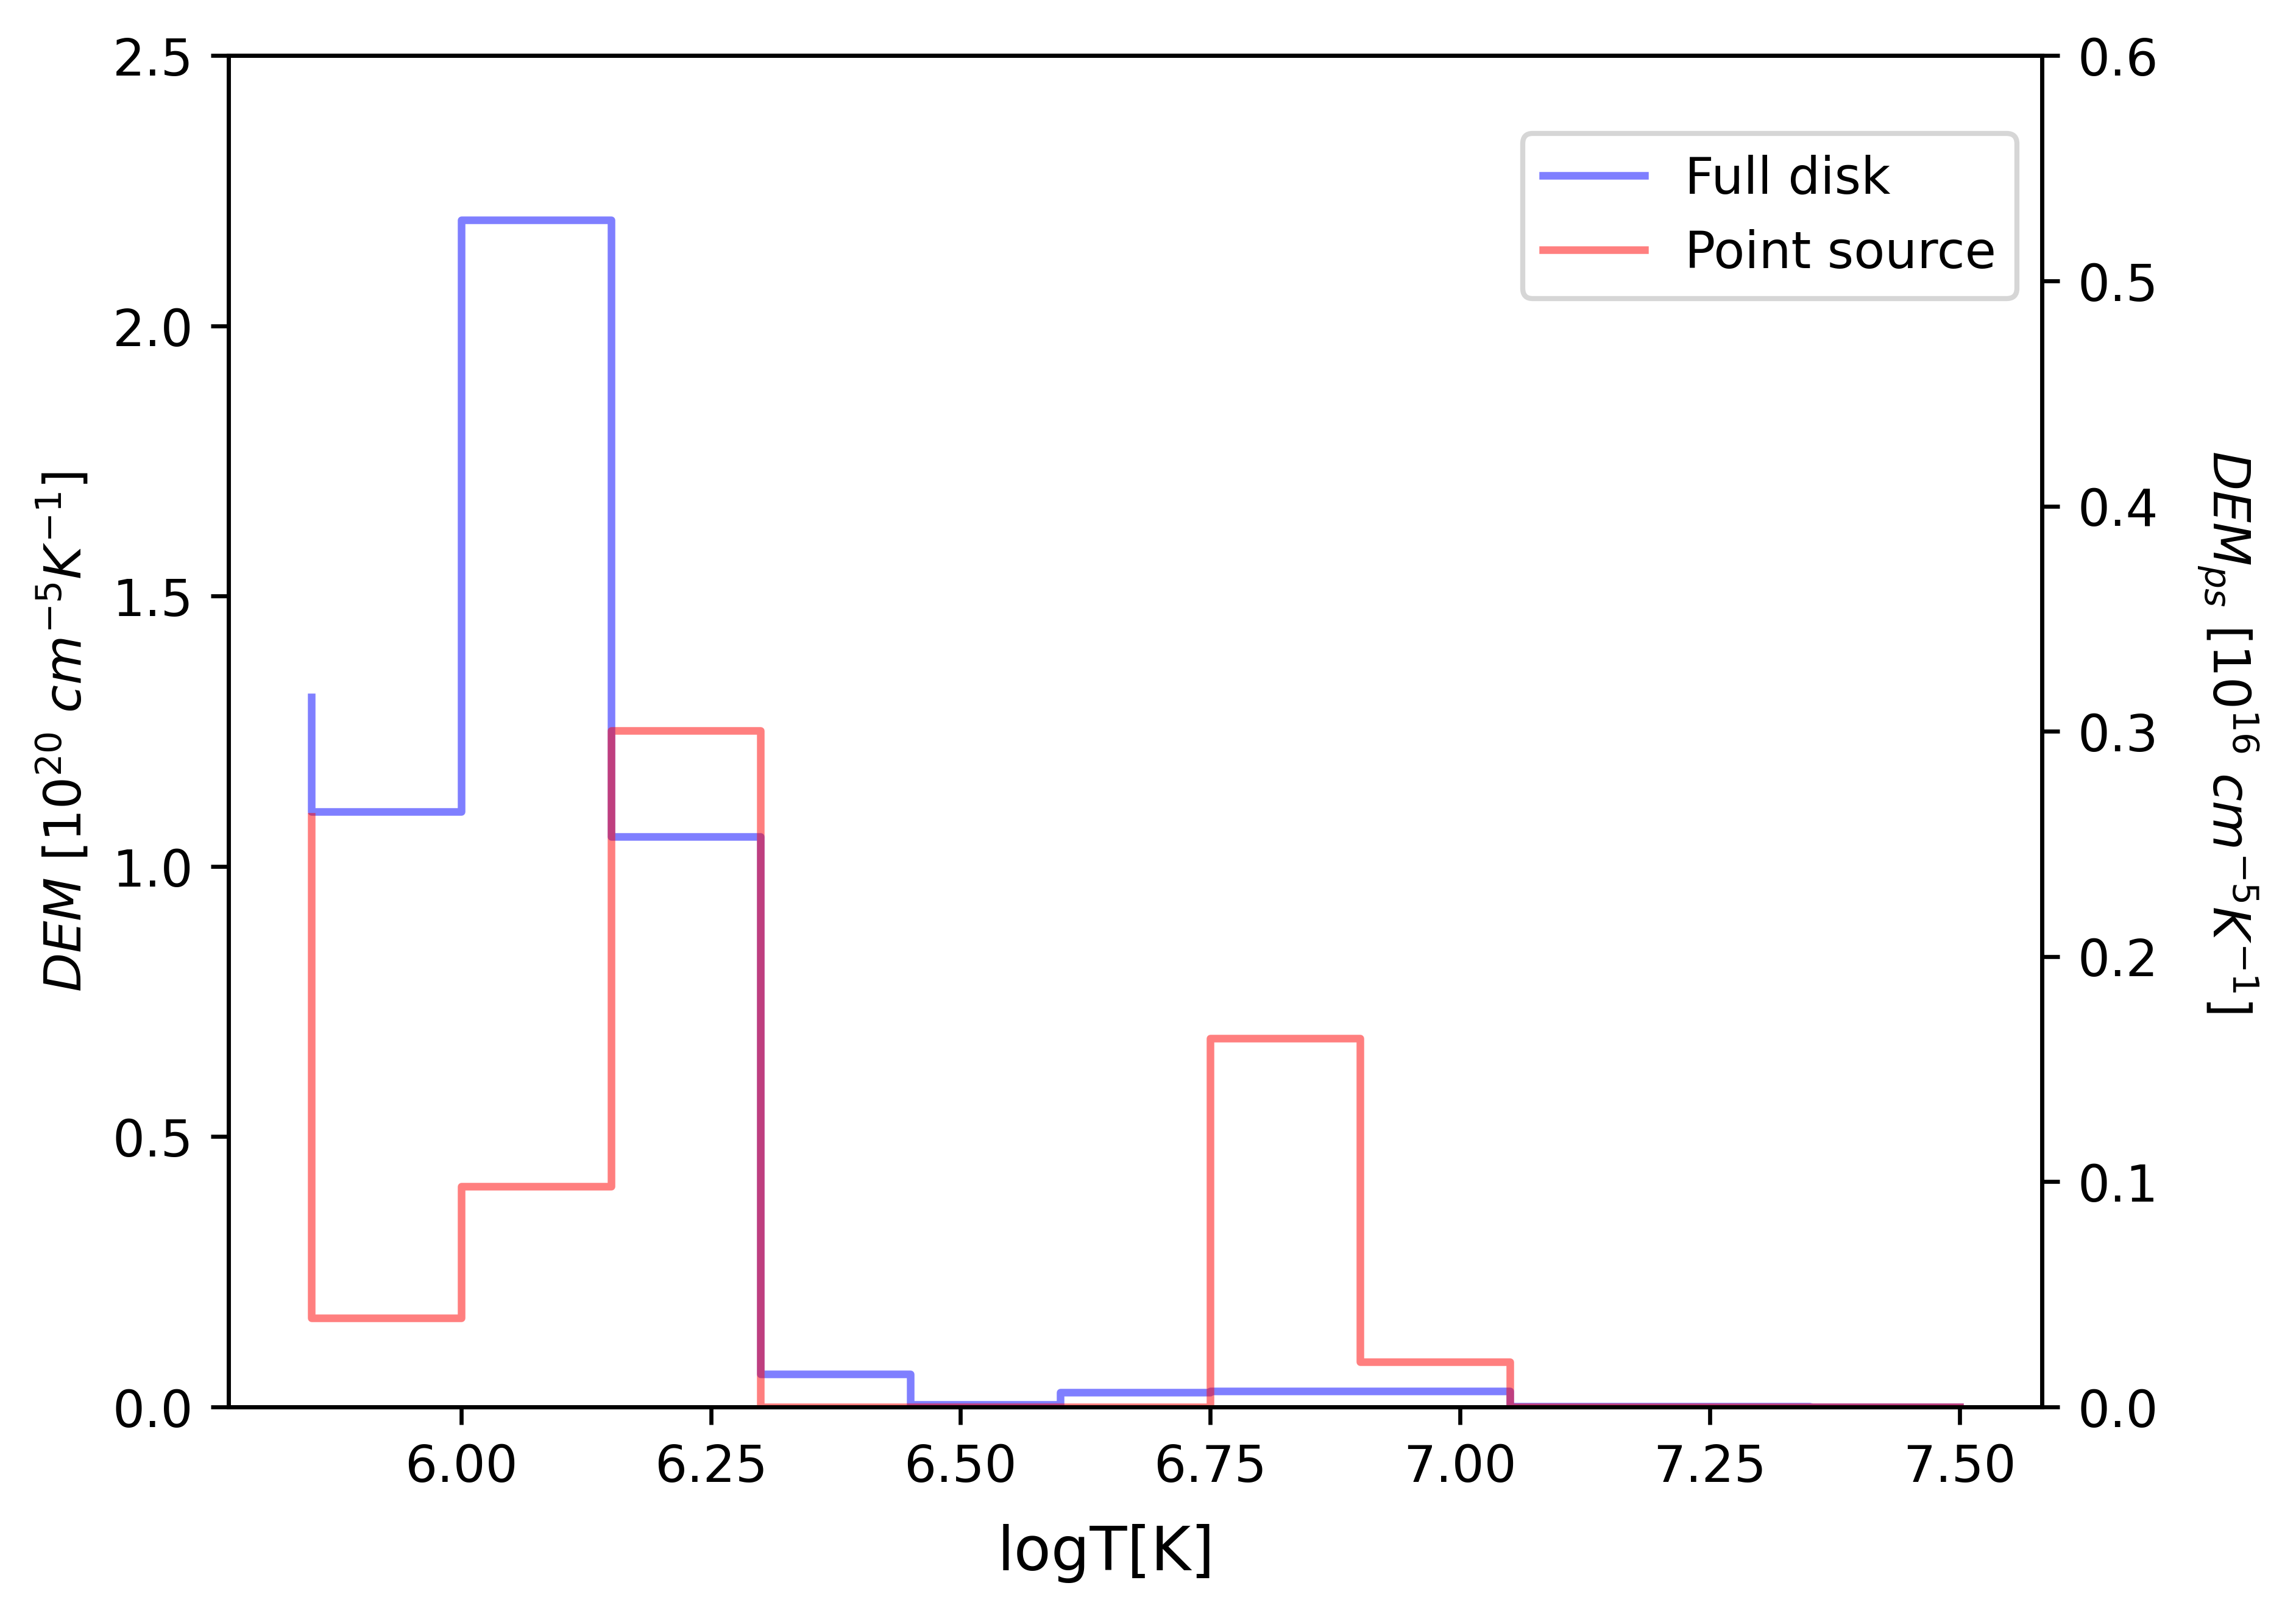
\includegraphics[width=\textwidth]{images/dem_profile_before_event_2021_oct_28.png}
        \caption{Before event (13:23 UT)}
    \end{subfigure}
    \hfill
    \begin{subfigure}[b]{0.3\textwidth}
        \centering
        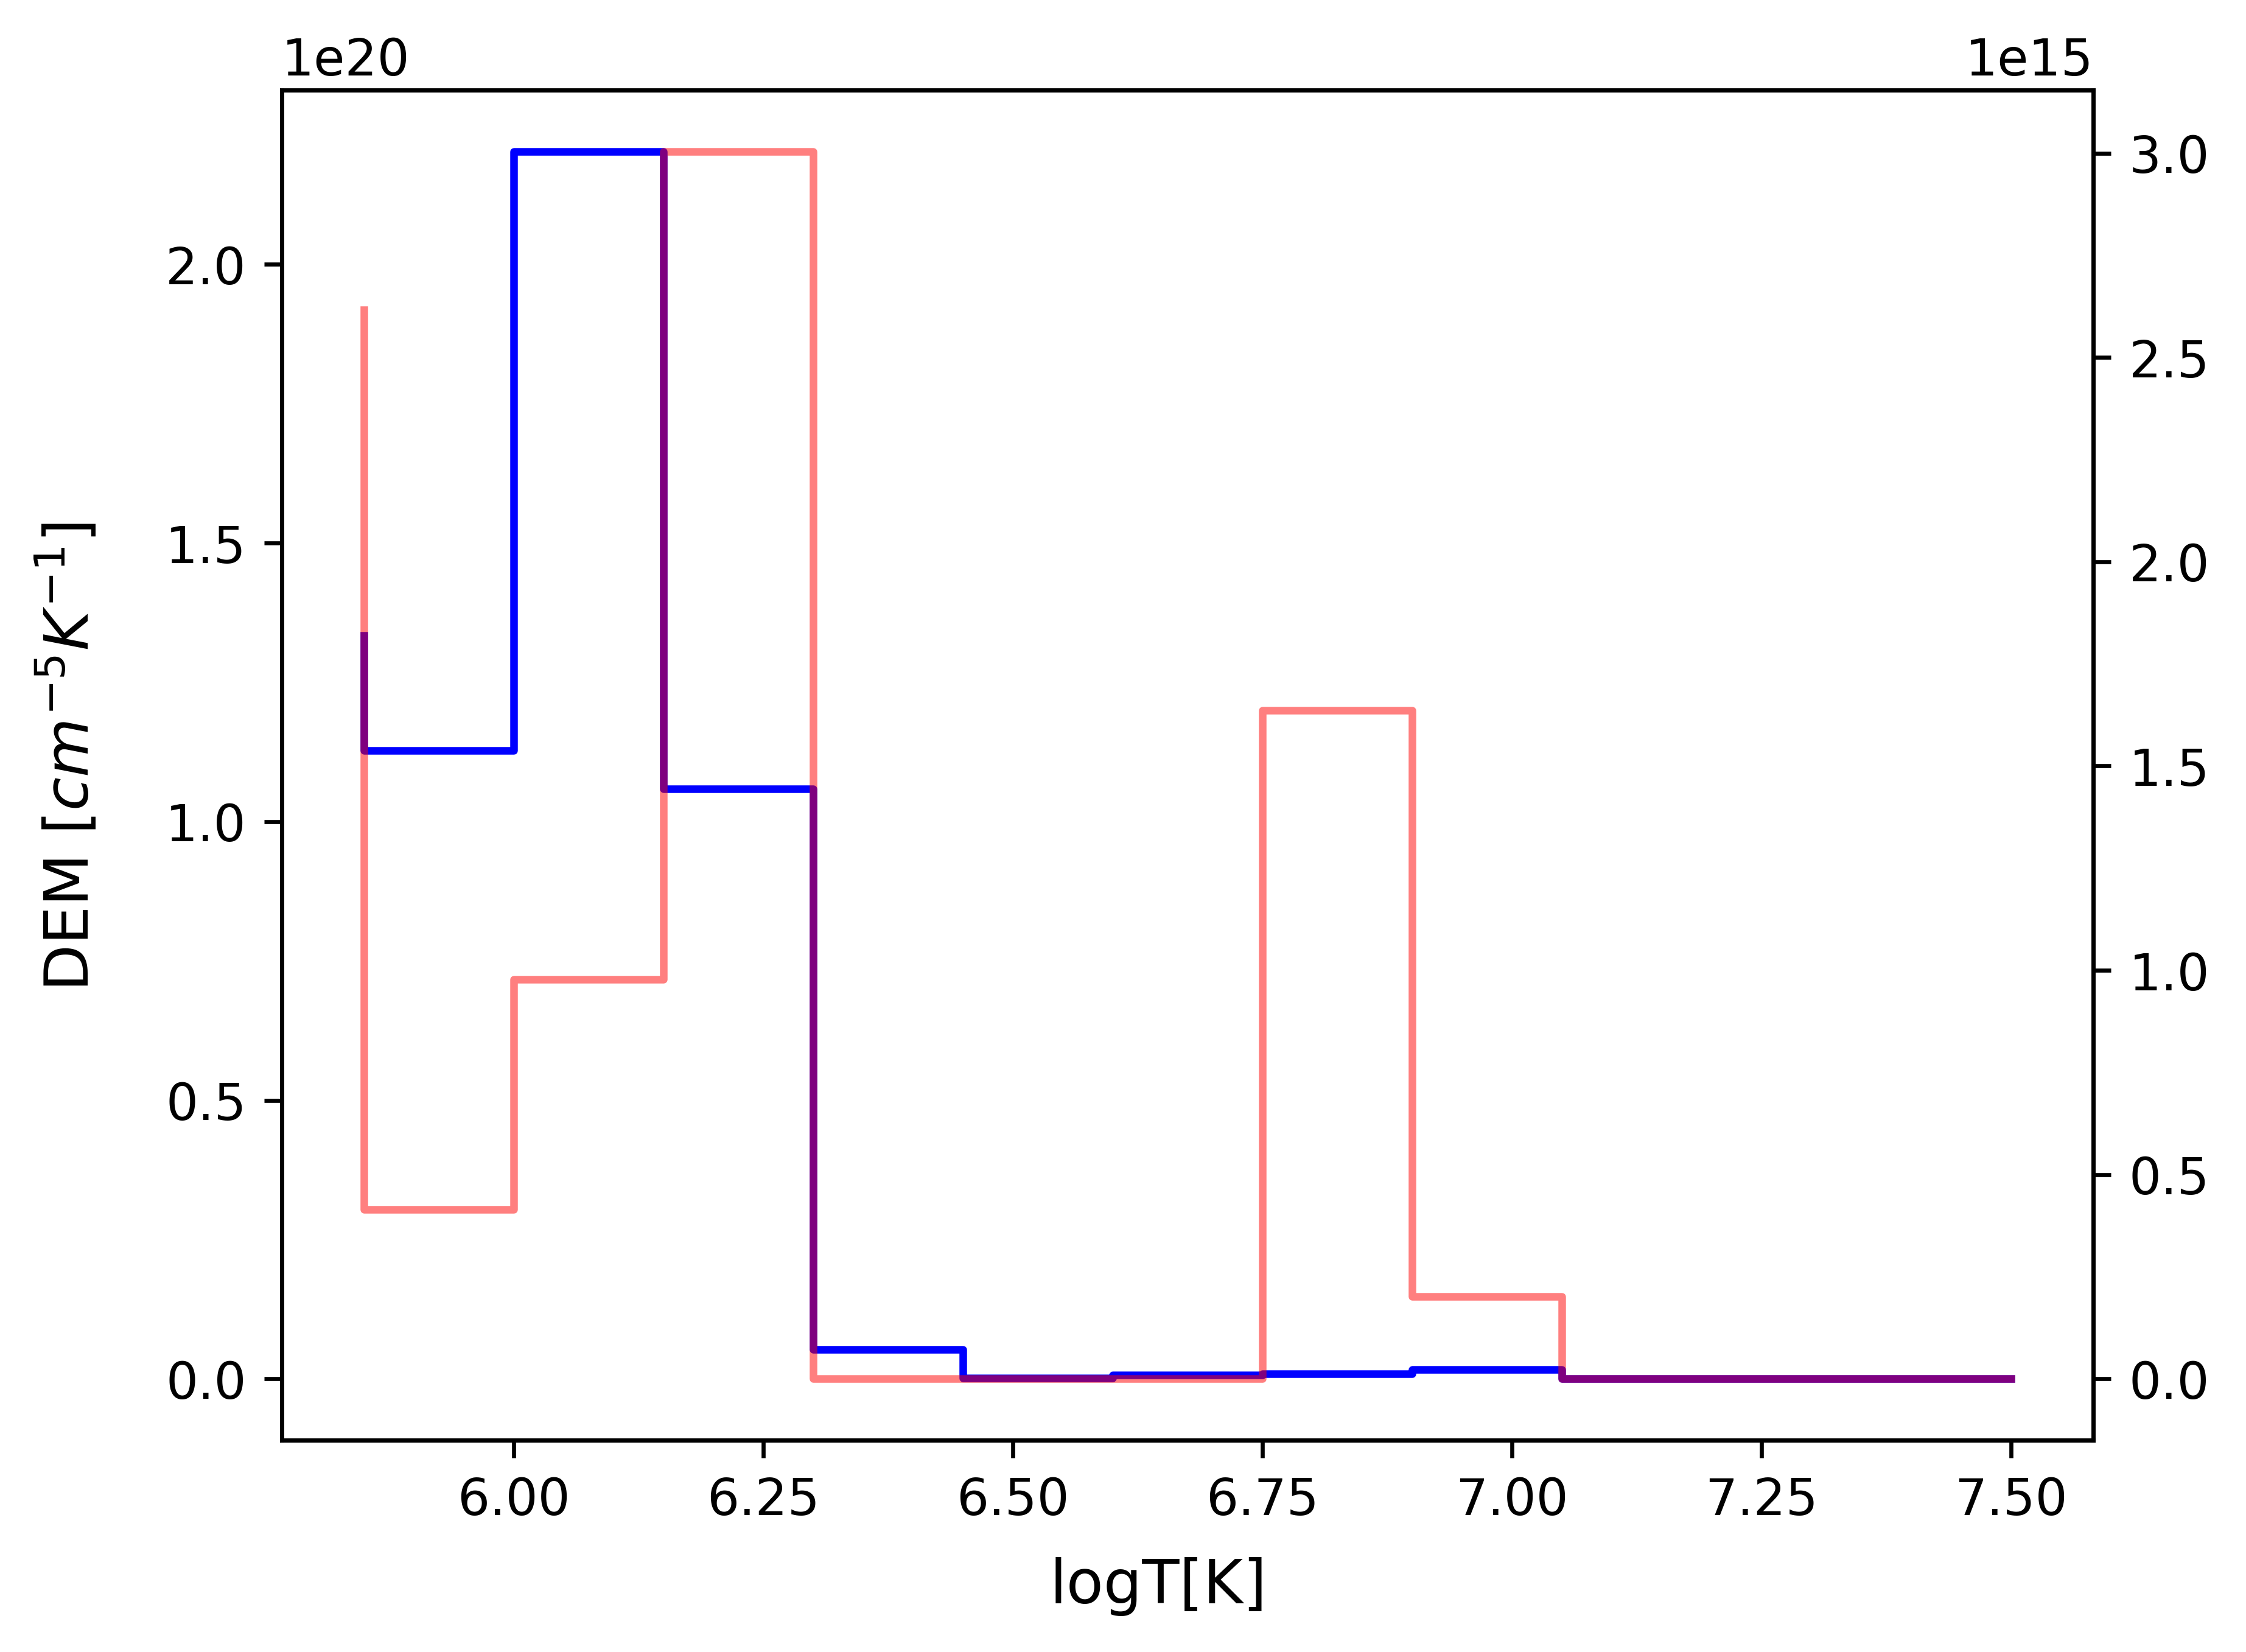
\includegraphics[width=\textwidth]{images/dem_profile_during_event_2021_oct_28.png}
        \caption{During event (15:17 UT)}
    \end{subfigure}
    \hfill
    \begin{subfigure}[b]{0.3\textwidth}
        \centering
        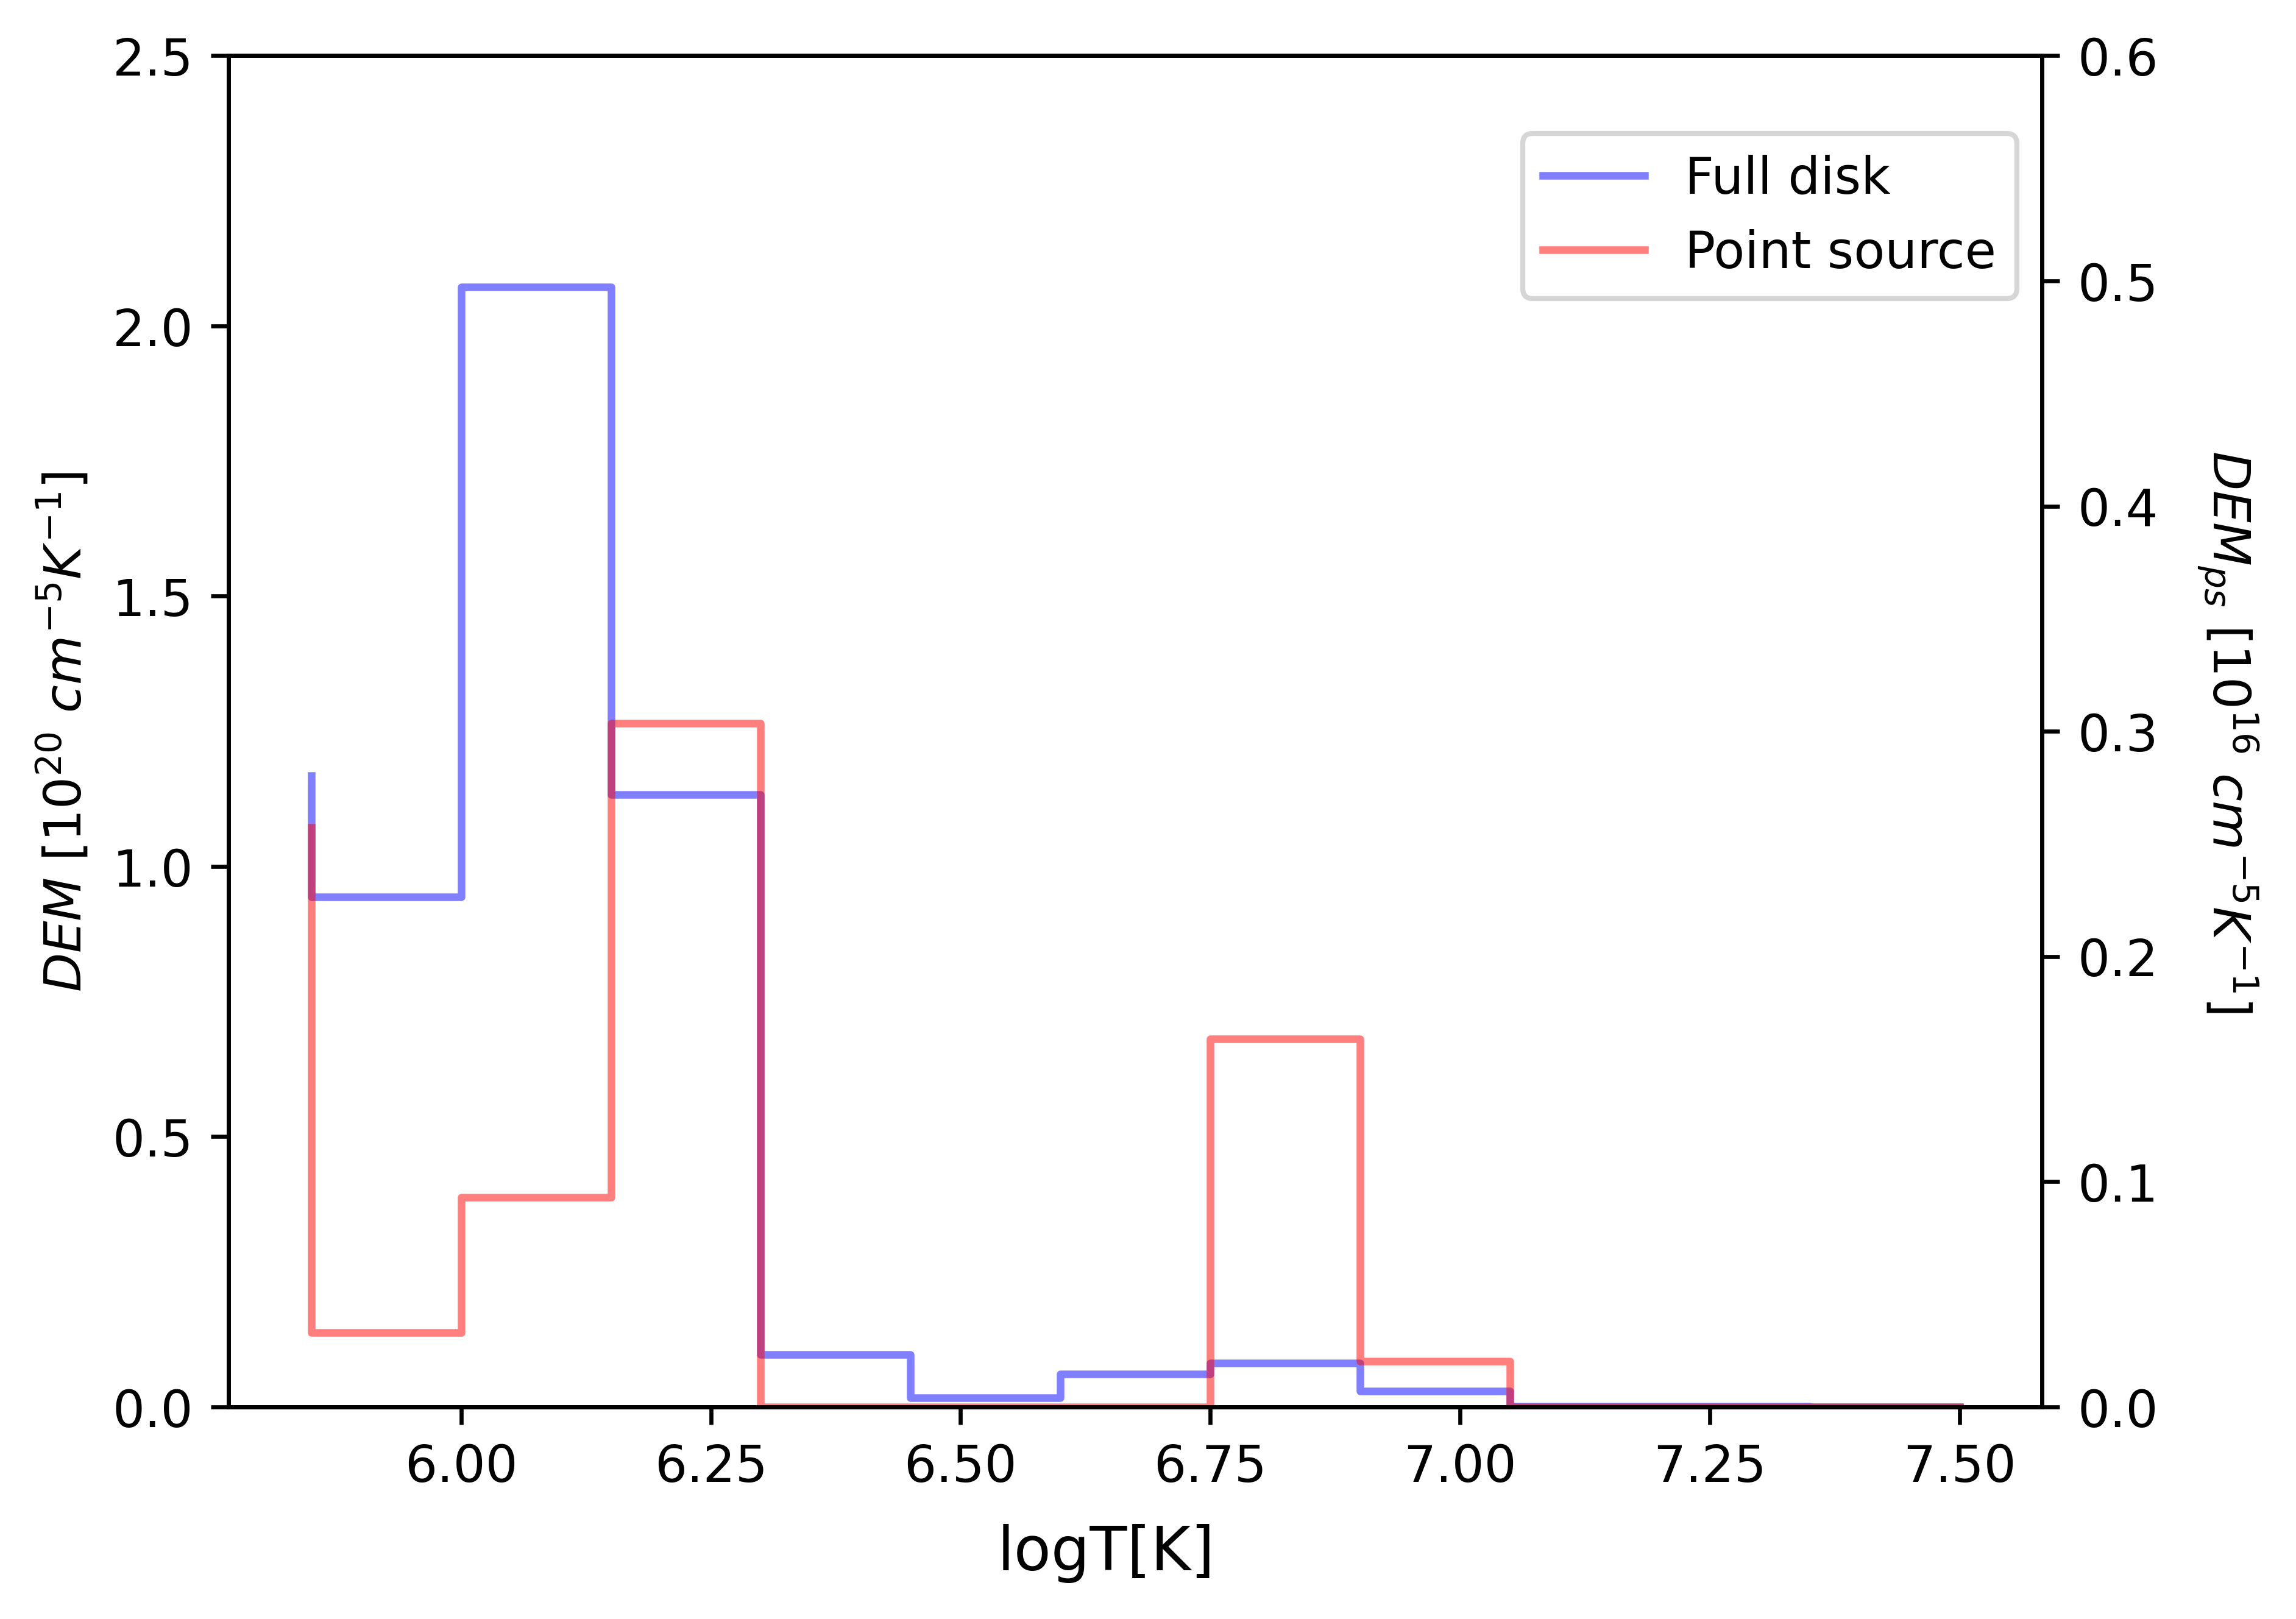
\includegraphics[width=\textwidth]{images/dem_profile_after_event_2021_oct_28.png}
        \caption{After event (17:29 UT)}
    \end{subfigure}

    \caption[DEM profile for \nth{28} October 2021 event]{DEM profile before, during and after the flaring event of \nth{28} October 2021. The red and blue curves correspond to point source and full disk source respectively}
    \label{fig:dem_pro_oct_28_2021}
\end{figure}


%%% Local Variables:
%%% mode: LaTeX
%%% TeX-master: "main"
%%% End:


\newpage
\section{Publications and Conferences}

\begin{itemize}

        \item Manuscript of this work is under preparation to be submitted to the The Astrophysical Journal.

        \item Best poster presentation award for the poser titled ``Could AI/ML help yield loss in Millets?'' at the two-days Scientific Extravanaganza `MilICon-2023', an International Conclave on Millets, held at Jain (Deemed-to-be University) - School Of Sciences, Bengaluru.

        \item Paper titled ``Crop Health Managemenet in Millets using Satellite Imagery and Neural Networks'' has been submitted to VEGETOS: An International Journal of Plant Research & Biotechnology. The paper is currently under review for publication.

        \item Poster presentation for the paper titled ``Crop Health Management in Millets using Satellite Imagery and Neural Networks'' was presented at the National Space Science Symposium 2024 Conference, Goa University.

\end{itemize}

%%% Local Variables:
%%% mode: LaTeX
%%% TeX-master: "main"
%%% End:


\newpage
\printbibliography

\end{document}

%%% Local Variables:
%%% mode: LaTeX
%%% TeX-master: t
%%% End:
